%!Mode:: "TeX:System

%%%%%%%%%%%%%%%%%%%%%%%%%%%%%%%%%%%%%%%%%%%%%%%%%%%%%%%%%%%%%%%%%%%%%%%%%%%%%
%                                                                           %
%          LaTeX File for Doctor (Master) Thesis of ECNU                    %
%            华东师范大学博士(硕士)论文模板 ____lizb                           %
%                                                                           %
%%%%%%%%%%%%%%%%%%%%%%%%%%%%%%%%%%%%%%%%%%%%%%%%%%%%%%%%%%%%%%%%%%%%%%%%%%%%%




\documentclass[12pt,openany,a4paper,fancyhdr,twoside]{ctexbook}

%draft 选项可以使插入的图形只显示外框,以加快预览速度。
\usepackage{amsmath}
\usepackage{amssymb}               % AMSLaTeX宏包 用来排出更加漂亮的公式

\usepackage[hyphens]{url}
\urlstyle{same}
\usepackage[hidelinks,breaklinks]{hyperref}

\usepackage{shortvrb,indentfirst,ulem,makeidx}
\usepackage{fancyhdr}
\usepackage{graphicx}

\usepackage{rotating}

\usepackage{indentfirst,latexsym,colortbl,clrscode}

% sudo code related.
\usepackage[linesnumbered,ruled,vlined,resetcount,algochapter]{algorithm2e}
\usepackage{algorithmicx}
\usepackage{listings}
\usepackage{algcompatible}
\usepackage{algpseudocode}


\renewcommand*{\algorithmcfname}{算法}

\newcommand{\clearPaperPage}{\clearpage}

\SetKwInput{KwIn}{\textbf{输入}}
\SetKwInput{KwOut}{\textbf{输出}}
\SetKwInput{KwReturn}{\textbf{return}}


\usepackage{bm}                     % 处理数学公式中的黑斜体的宏包
\usepackage{amssymb}                % AMSLaTeX宏包 用来排出更加漂亮的公式
\usepackage{mathrsfs}
\usepackage[subnum]{cases}
\usepackage[super,square,comma,sort&compress]{natbib}
\usepackage{hypernat}
\usepackage{geometry}
\usepackage{times}
\usepackage{fontspec}
\usepackage{libertineotf}
\usepackage{caption}
\usepackage{titletoc}
\usepackage{mathtools}

\counterwithout{footnote}{chapter}
\usepackage[perpage]{footmisc}       % 脚注每页重新编号

\usepackage{longtable,booktabs}
\usepackage{makecell}   % 表格内换行
\usepackage{multirow}
\usepackage{tocloft}
\usepackage{subfig}

\usepackage{float}
\usepackage{balance}
\usepackage{paralist}
\usepackage{bbding}
\usepackage{pgffor}

\usepackage{threeparttable}
\usepackage{threeparttablex}

\makeindex
\pagestyle{fancy}

\renewcommand{\headrulewidth}{0.4pt}
\fancyfoot[CO,CE]{\thepage}

\renewcommand{\algorithmicrequire}{\textbf{Input:}}
\renewcommand{\algorithmicensure}{\textbf{Output:}}

\newcommand{\yihao}{\fontsize{26pt}{36pt}\selectfont}           % 一号, 1.4 倍行距
\newcommand{\erhao}{\fontsize{22pt}{28pt}\selectfont}          % 二号, 1.25 倍行距
\newcommand{\xiaoer}{\fontsize{18pt}{18pt}\selectfont}          % 小二, 单倍行距
\newcommand{\sanhao}{\fontsize{16pt}{24pt}\selectfont}        % 三号, 1.5 倍行距
\newcommand{\xiaosan}{\fontsize{15pt}{22pt}\selectfont}        % 小三, 1.5 倍行距
\newcommand{\sihao}{\fontsize{14pt}{21pt}\selectfont}            % 四号, 1.5 倍行距
\newcommand{\banxiaosi}{\fontsize{13pt}{19.5pt}\selectfont}    % 半小四, 1.5 倍行距
\newcommand{\xiaosi}{\fontsize{12pt}{18pt}\selectfont}            % 小四, 1.5 倍行距
\newcommand{\dawuhao}{\fontsize{11pt}{11pt}\selectfont}       % 大五号, 单倍行距
\newcommand{\wuhao}{\fontsize{10.5pt}{15.75pt}\selectfont}    % 五号, 单倍行距

\newcommand{\tablewuhao}{\fontsize{10.5pt}{12.5pt}\selectfont}    % 五号, 单倍行距

\newcommand{\equwuhao}{\fontsize{11pt}{13.5pt}\selectfont}


\renewcommand*{\bibfont}{\normalfont\normalsize\linespread{1}\selectfont}


%============================ 可以自定义文字块 ================================%
\newcommand\mytool{FakeRevealer}
\newcommand\componentA{过滤模块}
\newcommand\componentB{鉴别模块}
\newcommand\componentC{代码分析模块}
\newcommand\componentD{人工审查}
\newcommand\componentE{应用特征库}

%交叉引用格式
\renewcommand\figureautorefname{图}
\renewcommand\tableautorefname{表}
\renewcommand\equationautorefname{式}
\renewcommand{\algorithmautorefname}{算法}

\renewcommand{\contentsname}{\hfill\bfseries\Large {目~~~~录}\hfill}
\renewcommand{\cftaftertoctitle}{\hfill}

\renewcommand{\listtablename}{\hfill\bfseries\Large 表~~~~格\hfill}
\renewcommand{\listfigurename}{\hfill\bfseries\Large 插~~~~图\hfill}
\renewcommand{\listalgorithmcfname}{\centering\bfseries\Large 算~~~~法}

% 章引用
\newcommand*{\fullref}[1]{\textbf{\hyperref[{#1}]{第\ref*{#1}章}}}
% 节引用
\newcommand*{\secref}[1]{\textbf{\hyperref[{#1}]{第\ref*{#1}节}}}
% 概念定义
\newtheorem{Def}{定义}


%=============================段前段后定义=============================%
\def  \cftbeforetitleskip {25pt}
\def \cftaftertitleskip {25pt}

%% 目录部分
\setlength{\cftbeforetoctitleskip}{\cftbeforetitleskip}
\setlength{\cftaftertoctitleskip}{\cftaftertitleskip}

%% 图目录
\setlength{\cftbeforeloftitleskip}{\cftbeforetitleskip}
\setlength{\cftafterloftitleskip}{\cftaftertitleskip}

%% 表目录
\setlength{\cftbeforelottitleskip}{\cftbeforetitleskip}
\setlength{\cftafterlottitleskip}{\cftaftertitleskip}

%% 算法目录
% \setlength{\cftbeforeloatitleskip}{\cftbeforetitleskip}
% \setlength{\cftafterloatitleskip}{\cftaftertitleskip}

\CTEXsetup[beforeskip=\cftbeforetitleskip]{chapter}
\CTEXsetup[afterskip=\cftaftertitleskip]{chapter}

%===============================概念定义===============================%
\newcommand{\citeline}[1]{[\citenum{ #1 }]}

\newcommand{\important}[1]{\CJKunderdot{\textbf{#1}}}

\newcommand{\code}[1]{\textit{ #1 }}
\newcommand{\codeInEqu}[1]{ {  \textit{\kaishu \textbf{#1 }}}}

\newcommand{\point}[1]{\subsubsection{\textbf{$\S$  #1 }}}
\newcommand{\Line}[1]{ \textit{ Line .#1}}

% 匿名开关
% \newcommand{\anonymous}[1]{\phantom{ #1 }}

% 查重开关
\newcommand{\duplicationCheck}[1]{\phantom{ #1 }}

% 查重自带匿名
\ifdefined \duplicationCheck
    \ifx \anonymous \undefined
        \newcommand{\anonymous}[1]{\phantom{ #1 }}
    \fi
\fi

% 基本信息
\newcommand{\TheisName}[0]{基于Android仿冒应用的大规模实证研究}
\newcommand{\TheisNameEn}[0]{A Large-Scale Empirical Study on Android Fake Apps}

\def\yearOfGrduation{2021} % 毕业年份
\def\monthOfGraduationNum{12} % 毕业月份
\def\monthOfGraduationEng{January} % 毕业月份 (英文)
\def\articleCategory{华东师范大学硕士学位论文} % 论文类型

\def\schoolNameChn{计算机科学与技术学院}
\def\schoolNameEng{School of Computer Science and Technology}

\ifdefined \anonymous
  \def\stuID{***********}
  \def\cmajor{*****}
  \def\cfield{*********}
  \def\cadvisor{***~**}
  \def\cname{***}

  \def\emajor{*****}
  \def\efield{*****}
  \def\eadvisor{***}
  \def\ename{***}
\else
  \def\stuID{51174506026}
  \def\cmajor{计算机科学与技术}
  \def\cfield{软件方法与程序语言}
  \def\cadvisor{\qquad 贺樑~教授 \quad 徐立华~副教授}
  \def\cname{唐~崇~斌}

  \def\emajor{\small{Computer Science and Technology}}
  \def\efield{\small{Software Method and Programming Language}}
  \def\eadvisor{\small{Prof.~Liang~He, A.P.~Lihua~Xu}}
  \def\ename{\small{Chongbin~Tang}}
\fi

% 基本信息 ends


%============================= 版芯控制 ================================%
\setlength{\oddsidemargin}{0.57cm}
\setlength{\evensidemargin}{\oddsidemargin}
\voffset-6mm \textwidth=150mm \textheight=230mm \headwidth=150mm
%\rightmargin=35mm

%============================= 页面设置 ================================%
%-------------------- 定义页眉和页脚 使用fancyhdr 宏包 -----------------%
% 定义页眉与正文间双隔线
\newcommand{\makeheadrule}{%
\makebox[0pt][l]{\rule[.7\baselineskip]{\headwidth}{0.4pt}}%
\rule[0.85\baselineskip]{\headwidth}{0.4pt} \vskip-.8\baselineskip}
\makeatletter
\renewcommand{\headrule}{%
{\if@fancyplain\let\headrulewidth\plainheadrulewidth\fi
\makeheadrule}} \makeatother

\newcommand{\adots}{\mathinner{\mkern 2mu%
\raisebox{0.1em}{.}\mkern 2mu\raisebox{0.4em}{.}%
\mkern2mu\raisebox{0.7em}{.}\mkern 1mu}}

\setmainfont{Times New Roman}
\dottedcontents{chapter}[1.5cm]{\xiaosi\heiti}{3.8em}{9.5pt}
\lhead{\articleCategory}

\dottedcontents{section}[1.5cm]{\xiaosi\heiti}{2.8em}{9.5pt}
\lhead{\articleCategory}

%=============================== 代码格式定义 ================================%


%% 辅助功能显示页边界
%\usepackage{showframe} % just for the example

\usepackage{etoolbox}

% thesis color scheme
\RequirePackage[table]{xcolor}
\definecolor{Strong Blue}{RGB}{6,64,194}
\definecolor{Dark Blue}{RGB}{6,46,139}
\definecolor{Night Blue}{RGB}{0,0,89}
\definecolor{Beige}{RGB}{219,212,192}
\definecolor{Dark Beige}{RGB}{185,170,129}
\definecolor{Night Beige}{RGB}{90,83,63}
\definecolor{Light Khaki}{RGB}{217,219,209}
\definecolor{Khaki}{RGB}{181,186,159}
\definecolor{Dark Khaki}{RGB}{113,117,99}
\definecolor{Light Red}{RGB}{214,124,118}
\definecolor{Red}{RGB}{212,24,14}
\definecolor{Night Red}{RGB}{105,18,12}
\definecolor{White}{RGB}{255,255,255}
\definecolor{Grey 1}{RGB}{238,238,238}
\definecolor{Grey 2}{RGB}{204,204,204}
\definecolor{Grey 3}{RGB}{170,170,170}
\definecolor{Grey 4}{RGB}{136,136,136}
\definecolor{Grey 5}{RGB}{102,102,102}
\definecolor{Grey 6}{RGB}{51,51,51}
\definecolor{Grey 7}{RGB}{33,33,33}
\definecolor{Black}{RGB}{0,0,0}
\definecolor{Frame Blue}{RGB}{0,85,128}
\definecolor{Frame Red}{RGB}{169,18,0}
\definecolor{Frame Green}{RGB}{55,143,23}
\definecolor{codegreen}{rgb}{0,0.6,0}
\definecolor{codegray}{rgb}{0.5,0.5,0.5}
\definecolor{codepurple}{rgb}{0.58,0,0.82}
\definecolor{backcolour}{rgb}{0.95,0.95,0.92}


\lstdefinestyle{mystyle}{
	frame=single,
	framexleftmargin=1.5em,
	commentstyle=\color{codegreen},
	keywordstyle=\color{magenta},
	numberstyle=\scriptsize ,
	stringstyle=\color{codepurple},
	basicstyle=\scriptsize,
	breakatwhitespace=false,         
	breaklines=true,                 
	captionpos=b,                    
	keepspaces=true,                 
	numbers=left,                    
	numbersep= 5pt,                  
	showspaces=false,                
	showstringspaces=false,
	showtabs=false,   
	xleftmargin=2em,       
	tabsize=2
}

% General style
\lstdefinestyle{normal}{
  aboveskip = 1.5em,
  backgroundcolor = \color{White},
   basicstyle = \ttfamily,
  belowskip = 1em,
   breakatwhitespace = false,
   breaklines = true,
   captionpos = b,
  commentstyle = \itshape\color{Dark Khaki},
  extendedchars = true,
  frame = lines,
  framerule = .6pt,
   framexleftmargin = 1em,
  framexrightmargin = 1em,
  gobble = 2,
  keywordstyle = \bfseries\color{Frame Blue},
  keywordstyle = [2]\bfseries\color{Frame Red},
  numbers = none,
  prebreak=\raisebox{0ex}[0ex][0ex]{\ensuremath{\hookleftarrow}},
  showspaces = false,
  showstringspaces = false,
  showtabs = false,
  stepnumber = 1,
  stringstyle = \color{Frame Green},
  tabsize = 2,
  upquote = true,
  xleftmargin = 1em,
  xrightmargin = 1em
}



% Cypher query language
\lstdefinelanguage{cypher} {
	keywords={start,create,set,delete,foreach,match,%
		where,with,return,skip,limit,order,by,asc,%
		ascending,desc,descending},
	morekeywords = {[2]type,id,length,nodes,rels,%
		relationships,abs,round,sqrt,sign,head,last,%
		tail,replace,left,right,substring,lower,upper,%
		ltrim,rtrim,trim,str,shortestpath,range,count,%
		sum,min,max,avg,collect,percentile\_cont,%
		percentile\_disc},
	sensitive = false,
	morecomment=[l]{//},
	morestring=[b]",
	morestring=[b]'
}


\lstset{style=mystyle}

\usepackage{bibspacing}
\setlength{\bibitemsep}{\baselineskip}
\renewcommand{\bibfont}{\normalfont}

\usepackage{lipsum}
% ADD THE FOLLOWING COUPLE LINES INTO YOUR PREAMBLE
\let\OLDthebibliography\thebibliography
\renewcommand\thebibliography[1]{
	\OLDthebibliography{#1}
	\setlength{\parskip}{0pt}
	\setlength{\itemsep}{0pt plus 0.3ex}
}

%=============================== 正文部分 ================================%

\begin{document}

\pagestyle{empty}
\setlength{\baselineskip}{25pt}  %%正文设为25磅行间距
\vspace{-2.0cm}
\noindent{{\zihao{4} {\large \yearOfGrduation} 届研究生硕士学位论文}}\\
\vspace{-0.8cm}
\begin{flushleft}
\hspace{-0.5cm}
\renewcommand\arraystretch{1.5}
\begin{tabular}{l}
\noindent{{\zihao{4} 分类号:\underline{\qquad\qquad\qquad\qquad}}}  \\
\noindent{{\zihao{4} 密~~~~级:\underline{\qquad\qquad\qquad\qquad}}}\\
\end{tabular}
\hskip 2.2 cm
\renewcommand\arraystretch{1.5}
\begin{tabular}{lc}
\noindent{{\zihao{4} 学校代码: }} & \underline{\qquad10269\qquad }\\
\noindent{{\zihao{4} 学\qquad 号: }} & \underline{~~~\stuID~~}\\
%\noindent{{\zihao{4} 学\qquad 号:\underline{\anonymous{51174506026}{ *** }}}}\\
\end{tabular}
\end{flushleft}


\vskip 1.0cm
\begin{center}
\scalebox{1.0}{
\includegraphics[width=2.08cm]{fig/ecnulogo.png}}  %原来为width=2.7cm
\hskip 0.5cm
\scalebox{1.0}{
\includegraphics[width=10.5cm]{fig/ecnulabel.png}}	%原来为width=10.5cm

{\textbf{{\xiaoer East China Normal University}}}\\ \vskip 0.2cm
\vskip 0.5cm
{\textbf{\erhao 硕~士~学~位~论~文}}\\ \vskip 0.2cm
{\textbf{\xiaoer MASTER'S DISSERTATION}}\\
\end{center}
\vskip 0.7cm

\begin{center}

{\erhao \bf 论文题目:}
\vskip 0.3cm
{\erhao \bf \underline{~\TheisName}}
\end{center}

\vskip 0.7cm
\begin{center}

\renewcommand\arraystretch{1.5}
\begin{tabular}{l}
{\sihao \bf 院\qquad\ \ \ 系:}\\
{\sihao \bf 专~业~名~称:}\\
{\sihao \bf 研~究~方~向:}\\
{\sihao \bf 指~导~教~师:}\\
{\sihao \bf 学位申请人:}
\end{tabular}
\begin{tabular}c
{\sihao \bf   \schoolNameChn}                \\
\hline {\sihao \bf  \cmajor }                \\
\hline {\sihao \bf \cfield }                 \\
\hline {\sihao \bf \cadvisor}              \\
\hline {\sihao \bf \cname }                  \\
\hline
\end{tabular}


\end{center}

\vskip 1.5cm
\begin{center}
{\sihao \yearOfGrduation 年 \monthOfGraduationNum 月}
\end{center}

\clearPaperPage



\pagestyle{empty}

\begin{flushleft}
	\large
	\renewcommand\arraystretch{1.5}
	\begin{tabular}{l}
		\noindent{\large Dissertation for master degree in 2019}  \\ 
		\noindent{\large  (Professional)}\\ 
	\end{tabular}
\qquad
	%\renewcommand\arraystretch{1.5}
	\begin{tabular}{lc}
	 University Code:  &  10269  \\ 
 Student ID: &    *****  \\ 
		%\noindent{{\zihao{4} 学\qquad 号:\underline{\anonymous{51164500190}{ *** }}}}\\ 
	\end{tabular}
\end{flushleft}

\vskip 2cm

\begin{center}
{\Huge $\mathbf{EAST}\,\mathbf{CHINA}\,\mathbf{NORMAL}\,
\mathbf{UNIVERSITY}$}
\end{center}

\vskip 3cm

\begin{center}
\bfseries{\scshape{\huge \TheisNameEn
}}\\
\end{center}

\vskip 2cm {\large
\begin{center}
\begin{tabular}{l}
Department:\\
Major:\\ 
Research Direction:\\
Supervisor:\\
Candidate:
\end{tabular}
\begin{tabular}c
\small	{{School of Computer Science and Software Engineering}}\\
\hline ~~~{***}  \\
\hline ~~~{***}\\
\hline ~~~{***}\\
\hline ~~~ {***}\\
\hline
\end{tabular}
\end{center}}

\vskip 30mm

\begin{center}
{\Large Sept, 2018}
\end{center}

\clearPaperPage

% 原创性声明。查重时不编译
\ifx\duplicationCheck \undefined
    \pagestyle{empty}
\centerline{\bf\Large 华东师范大学学位论文原创性声明}

\vskip 0.6cm

\normalsize \indent
郑重声明:本人呈交的学位论文《\TheisName》,是在华东师范大学攻读硕士/博士(请勾选)学位期间,在导师的指导下进行的研究工作及取得的研究成果。除文中已经注明引用的内容外,本论文不包含其他个人已经发表或撰写过的研究成果。对本文的研究做出重要贡献的个人和集体,均已在文中作了明确说明并表示谢意。

\vskip 0.6cm

\qquad\qquad{作者签名}:$\underline{\qquad\qquad\qquad }$
\qquad \qquad\qquad \mbox {日期}:\qquad 年 \qquad  月 \qquad  日


\vskip 0.8cm

\centerline{\bf\Large 华东师范大学学位论文著作权使用声明}

\vskip 0.6cm
《\TheisName》系本人在华东师范大学攻读学位期间在导师指导下完成的硕士/博士(请勾选)学位论文,著作权归本人所有。
本人同意华东师范大学根据相关规定保留和使用此学位论文,并向主管部门和学校指定的相关机构送交学位论文的印刷版和电子版;
允许学位论文进入华东师范大学图书馆及数据库被查阅、借阅;
同意学校将学位论文加入全国博士、硕士学位论文共建单位数据库进行检索,将学位论文的标题和摘要汇编出版,采用影印、缩印或者其它方式合理复制学位论文。


本学位论文属于(请勾选)

( ~)1.经华东师范大学相关部门审查核定的“内部”或“涉密”学位论文*,
于  ~~~~   年  ~~  月  ~~  日解密,解密后适用上述授权。

( ~ )2.不保密,适用上述授权。

\vskip 0.6cm

\qquad\qquad \mbox{导师签名}:$\underline{\qquad\qquad\qquad\qquad}$
\qquad\qquad \mbox {本人签名}:$\underline{\qquad\qquad\qquad\qquad }$

\vskip 0.3cm

$\rightline{ \qquad 年 \qquad  月 \qquad  日 \qquad\qquad}$

\vskip 0.6cm

\small{* “涉密”学位论文应是已经华东师范大学学位评定委员会办公室或保密委员会审定过的学位论文(需附获批的《华东师范大学研究生申请学位论文“涉密”审批表》方为有效),未经上述部门审定的学位论文均为公开学位论文。此声明栏不填写的,默认为公开学位论文,均适用上述授权)。}

    \clearPaperPage
\fi

\pagestyle{empty}
$$\\ \\ \\ $$

\centerline{\bf\Large $\underline{\mbox{\cname}}$硕士学位论文答辩委员会成员名单}

\vskip 10mm

\ifdefined \anonymous
	\def\nameProfA{***}
	\def\titleProfA{***}
	\def\nameProfB{***}
	\def\titleProfB{***}
	\def\nameProfC{***}
	\def\titleProfC{***}
	\def\affiliationA{******}
	\def\affiliationB{******}
	\def\affiliationC{******}
\else
	\def\nameProfA{章炯民}
	\def\titleProfA{副教授}
	\def\nameProfB{窦亮}
	\def\titleProfB{副教授}
	\def\nameProfC{钱莹}
	\def\titleProfC{副教授}
	\def\affiliationA{华东师范大学计算机科学与技术学院}
	\def\affiliationB{华东师范大学计算机科学与技术学院}
	\def\affiliationC{华东师范大学计算机科学与技术学院}
\fi

\begin{center}\large
	\begin{tabular}{ |p{25mm} < {\centering}|p{30mm} < {\centering}|p{48mm} < {\centering}|p{25mm} < {\centering}| }
		\hline
		\heiti  姓名 &\heiti  职称&\heiti  单位&\heiti  备注 \\
		\hline
		\nameProfA & \titleProfA & \affiliationA &  主席 \\
		\hline
		\nameProfB & \titleProfB & \affiliationB & \\
		\hline
		\nameProfC & \titleProfC & \affiliationC & \\
		\hline
	\end{tabular}
\end{center}

\clearPaperPage

\pagenumbering{roman}
\pagestyle{plain}

% 前置\cleardoublepage\phantomsection 以确保目录超链接到正确页码
\cleardoublepage\phantomsection\addcontentsline{toc}{chapter}{摘要}

\chapter*{\zihao{2}\heiti{摘~~~~要}}
\vspace{-5mm}

\setlength{\baselineskip}{25pt} % 25磅行距

Android移动操作系统由于其开源、用户广泛等特点,拥有庞大的应用生态环境,其中包含各种良性应用,以及恶意应用、重打包应用和仿冒应用。
得益于广泛的前人研究,业界对各类恶意、重打包应用具备充分理解,衍生出了对应检测机制与防护措施;
然而,近年来Android安全相关研究多聚焦于恶意、重打包应用,学术界对仿冒应用进行的研究较为匮乏,Android移动应用安全仍有隐患。

目前,针对仿冒应用的研究面临如下三点问题与挑战:
(1)业界尚缺乏一个公开可用的大规模仿冒应用数据集供研究者使用。其难点在于:收集数据时需要同时考虑数据规模、来源多样性与代表性;
(2)业界对仿冒应用的概念较为模糊,仿冒应用的基本特征尚未明晰,进而阻碍后续的检测工作;
(3)仿冒应用作者的行为特征尚不明确,无法为业界预防或拦截仿冒应用提供有效指导。

为获得关于仿冒应用的原始资料,本文采取实证研究的方式,从以下四个方面对仿冒应用进行了深入的分析和研究:

\textbf{通过收集大规模仿冒应用样本集,改善仿冒应用数据稀缺问题。}
本研究从应用宝、豌豆荚等多个应用来源入手爬取数据,最终筛选出5万个余个仿冒应用,可为后续工作如应用特征提取、应用行为分析等提供数据支持。

\textbf{针对Android仿冒应用特征进行多方面分析研究。}
利用上述数据集,本文对仿冒应用进行了与原版应用的相似度比对、功能比对等多方面解析,提供了仿冒应用的基本特征解读结果,并提供案例分析。
分析结果可为普通用户与应用市场等群体抵御仿冒应用威胁提供指导。

\textbf{利用证书信息与应用发布时间提供应用开发者行为画像。}
结合仿冒样本发布时间和从仿冒样本中抽取出的应用证书信息,本文从活跃期、投放特征等角度对仿冒应用开发者开展了一系列行为画像,该画像反映的行为特征可为应用市场提供监管思路。

\textbf{提出了可用的仿冒应用排查框架。}
实证研究表明,国内应用市场尚未有应对仿冒应用的完善措施。
针对该现状,本文推出了检测框架\mytool ,帮助应用市场在大规模应用中实现对已知正版应用及其对应仿冒样本的快速鉴别。

综上,本研究收集了较大规模数据集,可为后续工作提供数据支持和探索方向。
同时,依托收集到的大量数据,本研究对仿冒应用进行了全面分析,对普通用户和应用市场均提出了对应的实用建议,并提出了可行的检测方案,有助于提升各方对仿冒应用的认识与重视。

\sihao{\heiti{ 关键词:}} \xiaosi{Android应用程序, 仿冒应用, 实证研究, 数据分析, 排名欺诈}

\clearPaperPage

% \newpage

\addcontentsline{toc}{chapter}{ABSTRACT}
\vspace{-500pt}

\chapter*{\zihao{2}\heiti{ABSTRACT}}


%伴随着移动应用迅猛的发展,研究人员开始关注如何分析移动应用的业务逻辑,了解应用的运行行为。
%不同于传统应用程序,Android应用程序采用的是基于事件驱动的系统架构和面向组件的编程模式,业务逻辑对回调函数和多线程交互的依赖性高。
%上述特性使得程序的业务逻辑分散在不同的代码片段(例如方法、线程、组件等)中,阻碍了应用程序执行过程的建模,对了解Android应用程序执行细节造成了挑战。


With the rapid development of mobile apps, researchers have focused their attention on  mobile apps analysis.
They want to know the runtime behavior for the application via technical approaches.
Unlike traditional programs, Android apps, based on  event-driven architecture,  take the components like Activity as  essential building blocks and  rely on callback functions and multithreaded communication heavily.
These Android features split the business logic into diffrent segments, i.e., methods, threads, and components,  making trouble to the modeling for application execution , and  posing the challenge to understand the execution for Android apps.



%为此,本文提出并实现了一个可用于生成Android应用程序动态函数调用图的系统——RunDroid。
%RunDroid使用源程序代码插桩获取用户方法的执行信息,通过运行时方法拦截获取获取系统方法的执行信息,将这些信息以日志的形式保留下来。
%根据应用程序运行期间产生的日志信息,RunDroid能还原出应用的动态函数调用图。
%RunDroid构建的函数调用图不仅反映了函数间的调用关系,还能反映方法对象关系和方法间的触发关系,体现Android中Activity组件的生命周期,为程序分析工作提供必要的运行时信息。


This paper proposed  RunDroid, a system which can be used to build the dynamic function call graphs for Android apps.
RunDroid obtains  the execution information of user-level method via  the source-code level instrumentation,
gains the information of system-level method by runtime intercept.
Using the log information, generated while app running, RunDroid can recover the dynamic function call graph for the application.
The call graph, constructed by RunDroid, not only shows the calling relationship, but also reflects the method-object relationship, the trigger relationship between the methods, and the lifecycle of  Activity component, 
and provides the important runtime details for program analysis.





In this paper, we download 9 Android apps from the open source community F-Droid and use RunDroid to build dynamic function call graphs.
Results show that the trigger relationship is ubiquitous during app running and plays the major role in the Android.
Also, we compare the call graphs generated by RunDroid and FlowDroid.
Compared with the FlowDroid's static call graph, the dynamic call graph generated by RunDroid can accurately display the execution detail for the apps, express the calling relationship and trigger relationship between functions, and restore the lifecycle of the Android component Activity.
Finally, we apply RunDroid to fault localization for exploratory experiments.
The result shows that the call graph provided by RunDroid can  reflect the causal relationship of function execution comprehensively.
Compared with the previous technical, RunDroid makes the causal relationship model between methods more complete, and computes more program dependency information, which helps to improve the accuracy of fault location result.






{\sihao{\textbf{\newline Keywords:}}} \textit{Android, Call Graph, Dynamic Analysis, Lifecycle, Multi-Thread}



































% \clearPaperPage

\phantomsection\addcontentsline{toc}{chapter}{目录}
%%%%%%%%%%%%%%%%%%%%%%%%%%%%%%%%%%%%%%%%%%
%                                                             目录                                                         %
%%%%%%%%%%%%%%%%%%%%%%%%%%%%%%%%%%%%%%%%%%

\setcounter{tocdepth}{2}
\tableofcontents

\clearPaperPage


%%%%%%%%%%%%%%%%%%%%%%%%%%%%%%%%%%%%%%%%%%
%                  插图                  %
%%%%%%%%%%%%%%%%%%%%%%%%%%%%%%%%%%%%%%%%%%



\let\origaddvspace\addvspace
\renewcommand{\addvspace}[1]{}
%\setlength{\baselineskip}{30pt}  %%正文设为25磅行间距
\renewcommand{\cftfigpresnum}{图}
\setlength{\cftfignumwidth}{3em}

\listoffigures

\clearPaperPage

%%%%%%%%%%%%%%%%%%%%%%%%%%%%%%%%%%%%%%%%%%
%                                                             表格                                                         %
%%%%%%%%%%%%%%%%%%%%%%%%%%%%%%%%%%%%%%%%%%

\renewcommand{\cfttabpresnum}{表}
\setlength{\cfttabnumwidth}{3em}

\listoftables

% %%%%%%%%%%%%%%%%%%%%%%%%%%%%%%%%%%%%%%%%%%
%                 算  法                  %
%%%%%%%%%%%%%%%%%%%%%%%%%%%%%%%%%%%%%%%%%%

\renewcommand{\cfttabpresnum}{算法}
\setlength{\cfttabnumwidth}{3em}

\listofalgorithms

\clearPaperPage

\pagenumbering{arabic}
\pagestyle{fancy}
\fancyhead[LE,RO]{\small{\articleCategory}}
\fancyhead[RE,LO]{\small{\leftmark}}

\CTEXsetup[format+={\zihao{3}\heiti}]{chapter}
\CTEXsetup[format+={\raggedright\zihao{4}\heiti}]{section}
\CTEXsetup[format+={\zihao{-4}\heiti}]{subsection}

\setlength{\baselineskip}{25pt}  %%正文设为25磅行间距
\renewcommand{\addvspace}[1]{\origaddvspace{#1}} % 奇怪的section行间距。要放在这个位置
% 在章首页添加页眉

\fancypagestyle{plain}{%
    \fancyhead[LE,RO]{\small{\articleCategory}}
    \fancyhead[RE,LO]{\small{\leftmark}}
}

\raggedbottom
\xiaosi
\clearPaperPage

\chapter {绪论}
\label{chp:intro}

\section{研究背景}

随着移动市场于近年逐渐兴起,Android系统作为一个主流的移动端操作系统也在蓬勃发展。
数据分析机构StatCounter资料显示,Android市场占有率自发布之日起就在逐年稳步增长。
截至2020年,Android系统已经占据全球移动端市场份额的74.3\%~\cite{MobileOSMktShare}。
与此同时,Android应用\footnote{应用、App在本文中均用以指代Android应用程序,不再区分}的数量也伴随着Android市场的蓬勃发展节节攀高。
仅Android官方的应用商店Google Play就在2017年中新上架了近一百万个可供下载的应用程序。
虽然因为各种原因,Google Play上的应用数量在2018年有所回落,但如\autoref{fig:app_number}所示,应用市场上目前仍有近三百万个可用的应用程序,Android应用市场依然充满活力~\cite{StatistaAppNumber}。

\begin{figure}[htbp]
	\centering
	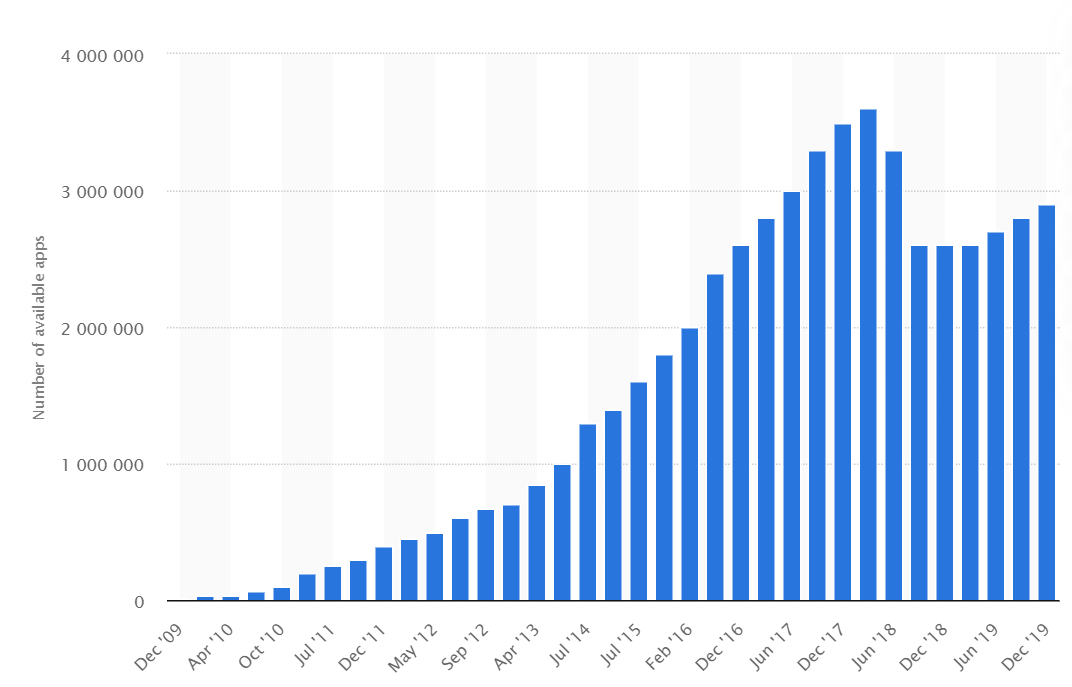
\includegraphics[width=0.9\textwidth]{./Figures/edwin-intro-app-number.png}
	\caption{Google Play 应用商店架上应用总数变化趋势}
	\label{fig:app_number}
\end{figure}

随着Android移动应用行业快速发展,移动黑灰产\footnote{即移动端黑色产业与灰色产业,下文同}也逐渐活跃。
黑灰产是以侵害用户、原应用作者或其他第三方利益为手段,凭此或通过其他可疑方式牟利的产业。
一方面,随着开发移动应用的门槛逐渐下降,开发一个移动应用的成本已经普遍低于开发一个类似的桌面级应用所需的成本~\cite{wasserman2010software};
另一方面,移动应用功能在实现上的灵活性~\cite{storydroid}增加了移动应用的复杂度,针对黑灰产的分析与拦截面临着多重新挑战。
两方面结合,为黑灰色应用进入移动端发展提供了良好的基础。

仿冒应用就是一类广泛存在的移动灰黑产产物。
本文研究的仿冒应用指代开发者根据市面上热门应用的外观仿制的Android应用。
据日常观察,仿冒应用中常有恶意广告弹窗、信息窃取、恶意扣费等行为,开发者可在用户使用仿冒应用时利用广告流量或非法获得的用户信息获利。
一方面,仿冒应用损害了原版应用开发者的知识产权,侵害了原开发者的利益;
另一方面,仿冒应用中的恶意行为也在威胁普通用户的信息安全。
可以联想如下场景:用户尝试通过应用市场搜索安装一个应用,应用市场返回了多个无论是名字或是图标都十分相像的结果,在未有明确指引的情况下,用户安装了仿冒应用。
前人针对Android恶意应用的研究~\cite{Zhou2012DissectingAM}显示,恶意行为可被自动触发,若用户下载的仿冒应用中包含此类恶意行为,用户数据安全将受到损害;
同时,由于用户不能分辨原版应用与仿冒应用,后者的不良用户体验会导致用户对前者乃至应用市场产生不良评价;
即使用户删除仿冒应用、装上原版应用,也浪费了时间和人力成本。

综上所述,仿冒应用影响用户搜索与下载应用时的安全和体验,最终使用户、原版应用开发者和应用市场三方利益均受到损害。
为了消除仿冒应用带来的隐患,无论是开发者、应用市场或是普通用户,都应对仿冒应用的特征与行为有所了解。

\section{研究现状}
尽管客观上存在对仿冒应用进行了解的需求,本研究对移动应用领域的前期调研显示,针对仿冒应用进行的实证研究尚缺乏,也未有公开可用的仿冒应用数据集。
因此,本节讨论与仿冒应用同属于移动灰黑产的重打包应用和恶意应用、以及其他移动应用领域相关方向的研究现状。

\subsection{重打包应用的研究现状}
\label{sec:repackaging}
重打包指恶意开发者对原应用解包、篡改内容之后再将应用重新打包的技术~\cite{khanmohammadi2019empirical}。
重打包应用侵害了应用原作者的知识产权,甚至可能具有恶意行为,因此也属于移动黑灰产范畴。
目前针对重打包应用的相关工作分为三类,分别为关于重打包的实证研究、针对重打包应用的检测和防止应用被重打包的研究。

相关实证研究方面,Khanmohammadi等人对重打包应用进行了一次详尽的实证研究~\cite{khanmohammadi2019empirical}。
该实证研究利用已有数据集AndroZoo~\cite{li2017androzoo++},得出了``重打包应用的主要目的为利用广告获得收入''的结论,并回答了包括``何种类型的应用会被重打包''、``重打包对原应用属性更改如何''在内的五个研究问题,增进了研究者对重打包应用的理解。


在重打包应用检测方面,早期工作通过比对两两应用之间的信息获得应用之间的相似度。
有研究者基于应用指令序列的方法使用模糊哈希的方法提取出应用的摘要信息,如DroidMOSS和DroidAnalytics~\cite{DroidMOSS, Zheng2013DroidAnalyticsA};
也有使用静态数据依赖构建程序依赖图(Program Dependency Graph, PDG)比对应用的方法,如DNADroid~\cite{DNADroid}和AnDarwin~\cite{AnDarwin},Centroid~\cite{Centroid}甚至为应用中的每个函数构建了三维控制流图(3-Dimensional Control Flow Graph, 3D-CFG),将三维控制流图聚合后,通过检测不同应用在控制图聚合后的质心位置判断应用间的相似程度;
还有算法通过比对抽象语义树检测重打包应用,如Hanna等人的Juxtapp~\cite{hanna2012juxtapp}利用K-gram模型对应用的二进制操作码序列进行比对,CLANdroid~\cite{CLANdroid}通过分析五种语义特征点(比如代码中的标识符和调用到的Android API等),以检测相似应用。
上述算法一来因为需要使用静态分析方法对代码进行解析,在遇到使用过代码混淆处理(如反射和代码加密)的应用时性能往往较差;二来需要基于两两比对进行检测,复杂度较高,在应用规模增大时会导致庞大的计算量。
为处理静态分析带来的问题,有学者提出了利用动态分析比对应用的方法,如Wu等人使用HTTP流量对应用行为进行建模~\cite{wu2015detect}。
亦有研究使用信息可视化方法检测重打包应用:ViewDroid~\cite{ViewDroid}通过重建和比对应用的视图筛出重打包应用,DroidEagle~\cite{sun2015droideagle}则利用UI布局相似性检测,Kywe等人比对应用中的文本与图像相似性以寻找相似应用~\cite{kywe2014detecting},Soh等人分析应用运行时收集的UI信息以检测重打包行为~\cite{soh2015detecting}。
而从避免两两比对、减小算法复杂度方面考虑,有学者提出利用第三方库进行检测的办法,如CodeMatch~\cite{CodeMatch}筛选出应用中使用的第三方库代码后,计算并比对剩余部分代码的哈希值,获取不同应用的相似程度;Wukong~\cite{Wukong}也分两步检测重打包应用,但与CodeMatch相比,其第二步使用了基于计数的代码克隆检测手段,而非基于哈希的技术。

防止应用被重打包的研究多基于检测原有代码是否被更改而开展。
Zhou等人提出了两个基于改版Dalvik虚拟机的对抗工具:其中,AppInk~\cite{zhou2013appink}利用一种``水印''技术(Watermarking)对抗重打包,但需要利用一个改版的Dalvik虚拟机进行文件检查;另一工具DIVILAR~\cite{zhou2014divilar}为应用的Dalvik代码提出了一种新编码形式,同时也需要修改用户设备Android系统中的Dalvik虚拟机以对新的编码进行解码。
Luo等人提出了在代码中注入大量检测节点的方法对抗重打包,并推荐开发者进行代码混淆,以避免令重打包开发者发现注入的检测节点~\cite{luo2016repackage}。
与之相似,Zeng等人也提出了在代码中注入逻辑炸弹的方法,并在研究中讨论了多种避免重打包开发者发现代码注入的策略~\cite{zeng2018resilient}。

\subsection{恶意应用的研究现状}
针对恶意应用的研究可分为两个方面,分别是面向恶意应用进行实证研究工作与面向恶意应用检测的研究。

面向恶意应用的实证研究众多,较有代表性的有以下两篇文献:
Felt等人的研究~\cite{Felt2011ASO}仔细剖析了来自多个不同平台的46个恶意程序样本以了解这些样本的激励机制,揭示了这些样本的运行机制和行为策略,为后人抵御此类恶意行为提供参考;
Zhou和Jiang~\cite{Zhou2012DissectingAM}搜集了来自多个主要恶意应用家族的、超过1,200个恶意应用样本,并系统性地描绘了这批样本的不同性质,包括其安装手段、激活机制和其如何执行有效负载(实现恶意行为)。
虽然恶意应用与仿冒应用有重合之处,但两者有一定区别,相关理论知识直接套用并不合适。

以上述实证研究与数据分析作为基础,研究者对恶意应用有了较好的了解,从而得以有针对性地进行恶意应用检测。
相关方法可大致分为静态分析、动态分析与机器学习三个方向。
早期研究通过静态分析手段对恶意应用进行检测,包括Enck等人提出的Kirin,在应用安装时检测应用权限,从而拦截恶意应用的安装~\cite{enck2009lightweight};
Felt等人提出的Stowaway~\cite{felt2011android}利用API调用分析和权限分析,寻找权限过大(Overprivileged)的应用;
RiskRanker~\cite{grace2012riskranker}则提出了一个两阶恶意应用检测手段,先筛选出具有root行为和可能导致隐私泄露的应用,再找出其中具有危险Dalvik代码加载行为的应用。
然而,受静态分析方法本身的限制,此类研究在遇到代码混淆时多被影响性能。
因此,有研究者利用动态分析技术对恶意应用进行检测。
TaintDroid~\cite{enck2014taintdroid}和DroidScope~\cite{yan2012droidscope}均在沙箱中对应用行为进行监视,TaintDroid利用污点分析技术寻找应用的信息泄露行为,DroidScope则从Android系统的不同层面分析应用的可疑行为。
Zhou等人\cite{zhou2012hey}提出了DroidRanger,利用应用行为比对与动态加载分析的方式,成功地从5个应用市场的204,040个应用中找出了211个恶意应用。
ParanoidAndroid~\cite{portokalidis2010paranoid}提出了将恶意检测方法迁移到云端的概念,将设备上的所有操作同步到云端服务器,从而在不影响设备本地功能的情况下进行恶意行为检测。
无论是静态分析方法或是动态分析方法,都需要人工对恶意行为的模式进行描绘,而用人工手段提取行为模式,不仅对领域知识有较高要求,还往往是费力费时的。
针对此问题,研究者开始利用机器学习技术检测恶意应用。
Chen等人从大规模数据集中总结出了恶意应用的两类特征,再将其用于分类器模型训练,提出了检测工具StormDroid~\cite{chen2016stormdroid},与之类似的方法还有CrowDroid~\cite{burguera2011crowdroid},DroidMat~\cite{wu2012droidmat},Adagio~\cite{gascon2013structural},MAST~\cite{chakradeo2013mast},DroidAPIMiner~\cite{aafer2013droidapiminer}与Drebin~\cite{arp2014drebin}。

\subsection{其他相关研究}
Andow等人针对灰色应用的研究~\cite{Andow2016ASO}从Google Play应用商店中采集了多个应用样本。
该研究将样本分类,定义了高仿应用(Imposter)、移动广告应用(Madware)等9种不同的灰色应用。
灰色应用指不具有明显恶意行为,但应用意图存疑、又或是会向系统申请过多权限的应用程序。
因此,这类应用不是恶意应用,但由于其盈利方式可疑,可将其归入移动黑灰产内。

另一方面,Hu等人针对市面上的欺诈约会应用进行了一次实证研究~\cite{hu2019dating}。
该研究中的欺诈约会应用声称自己为约会应用,实则诱导用户开通会员服务,也应归入黑灰产应用范畴。
分析发现,用户在此类应用中遇到的其他``用户''多数不由真人控制,而是具有预设对话模板的聊天机器人。
此外,研究还分析了该类应用的商业模式与分发渠道,评估了受害者的数量,对此类应用的生态进行了详尽解读。
该研究还通过直接检测相同评论和标记可疑用户的方式对此类应用进行排名欺诈检测。

Chen等人发布了漏洞检测工具Ausera~\cite{chen2018ausera},该工具通过静态分析技术与敏感词识别,对手机银行应用进行自动化三段式风险评估。
同期,他们在一个实证研究中利用Ausera从693个手机银行应用中检出超过两千个漏洞,向对应的60家银行发送了漏洞报告,并检查了新发行的手机银行应用以跟进漏洞修补进程~\cite{chen2018mobile}。
在被检出漏洞的60家银行中,21家确认了该研究反馈的漏洞,进行了对应修复,作者随后根据修复状况进行案例研究,分别面向银行、学者与政府,共给出了9条用于改善手机银行应用安全性与市场环境的实用建议。
与之类似,本研究也从多个方面出发,提出了防范仿冒应用、净化市场环境的实用建议。

% \subsection{针对应用评论的相关研究现状}
% 近年来,除了利用应用程序牟利以外,移动黑灰产业也开始进入应用市场评论的领域。
% 相关工作也可以分为检测与相关的实证研究两类。

% 检测方面,
% Zhu等人提出了一个利用评价历史记录检测应用是否具有排名欺诈行为的研究~\cite{zhu2014discovery}。
% 该研究提出,一般应用的排名在上升期(Raising phrase)和下降期(Recession phrase)之间会有一段维持期(Maintaining phrase),维持期过短且排名在短时间内剧烈波动的应用很可能具有排名欺诈行为。
% 然而,用该方法进行检测需要持续收集应用在市场上的评分数据,因此对数据采集有一定要求。
% Lim等人分析了差评水军(Review spammers)的特征并将其用于建模,以检测类似行为~\cite{lim2010detecting};
% Xie等人利用图论挖掘评论中开展共谋攻击(Collusion attack)的用户群组~\cite{xie2014grouptie},并在后续研究中将该方法拓展成一个检测系统~\cite{xie2016you}。
% 与之相似,Chen等人同样使用了基于图论的方法检测共谋攻击~\cite{chen2017toward},
% Hooi等人的FRAUDAR通过寻找二分图中的密集子图寻找关系特别密切的用户与应用,从而找出可能提供排名欺诈服务的可疑用户与使用了该服务的应用~\cite{hooi2016fraudar}。

% 实证研究方面,Rahman等人对Google Play中虚假评论行为的实证研究~\cite{rahman2019art}在公开确认该产业链存在的同时,也揭露了该产业的行为模式、生存情况甚至从业人员收入水平等方面的信息。

% 作为黑灰色产业链下游环节,虚假应用评论(即排名欺诈行为)已在前述研究中被证明与欺诈约会应用存在关联。
% 因此,排名欺诈也很可能与仿冒应用相结合,为移动黑灰产从业者牟取更多利益,有必要开展相关分析进行确认。

\subsection{研究现状小结}
综合上述分析,与仿冒应用同属黑灰产的重打包应用和恶意应用,甚至是日常生活中常用的手机银行类应用,均有对应研究可提供参考。
前人的实证研究收集了较为大量的重打包应用、恶意应用和手机银行应用数据,并提供了重打包应用与原版差异、恶意应用传播方式与负载执行方式、手机银行应用常见漏洞等指导性信息,帮助专业人员改善现有移动应用环境。
在丰富的前序研究提供的领域知识与数据支持下,各界才得以对重打包应用、恶意应用开展后续的检测研究。
相比之下,仿冒应用的相关数据和研究成果都乏善可陈。

换言之,在上述研究中,无论是对恶意应用还是重打包应用进行检测,都需要有一定领域知识或洞见(Insight)作为理论支撑。
对仿冒应用而言,学术界与工业界对其认知均较贫乏,``基于新见解进行技术拓展改良''式的研究手段尚未适用于仿冒应用。
因此,着眼于领域知识梳理的实证研究更适用于仿冒应用在当下的研究场景。
% \subsection{实证研究}
% 实证研究是一种基本研究技术,旨在针对特定方法在实际应用场景下的真实状况或对应产物进行数据收集、调查与分析,以让研究者了解事物的工作原理或使理论得以验证。
%
% 在软件工程领域,由于理论研究与工程实践结合较为紧密,学者采用需要检验理论在实践中的落地情况(如程序语言提供的特性是否被良好地理解与使用~\cite{bieman1995reuse}、是否在工程实践中体现优势等~\cite{harrison2000experimental}问题)或是调研现实应用场景中产生的现象(如恶意应用、重打包应用等在移动端市场出现的实际问题~\cite{Felt2011ASO, Zhou2012DissectingAM, Andow2016ASO, wang2018android}),实证研究技术是十分适合的方法。
% 因此,有越来越多的研究者使用实证研究技术对研究主体进行探索\cite{Felt2011ASO, Zhou2012DissectingAM, Andow2016ASO, wang2018android, chen2018ausera, chen2018mobile, bieman1995reuse, harrison2000experimental, dybaa2008empirical, manotas2016empirical, mcintosh2016empirical, mcilroy2016fresh, wu2016ji, yang2015xin, hu2019dating, khanmohammadi2019empirical}。
% 随着实证研究技术在软件工程领域中的认可度逐渐提高,软件工程顶级会议FSE与ICSE近年分别新设立了面向工业界的投稿分区,鼓励学者多基于应用场景进行实证研究,探明业界现状。
%
% 为向软件工程领域进行实证研究的学者提供方法论支持,Kitchenham等人基于自身在评阅软件工程项目的经验和一份针对医学研究者的研究指引,总结出了一份对于软件工程实证研究的初步准则(Preliminary guideline)~\cite{kitchenham2002preliminary},对实证研究的数据收集方法、实验设置方法等各个步骤都给出了严格指引,如在数据收集时需要确保数据的准确性与完整性,需要保证实验的可重复性等。
% 为保证数据的准确性与完整性,本研究利用\mytool 尽可能全面地收集多个来源的应用样本。
% Seaman则结合实例,提供定性分析的~\cite{seaman1999qualitative}。
% 在实证研究可采取的具体方式方面,Easterbrook等人于2008年提出了面向软件工程领域的实证研究方法建议~\cite{easterbrook2008selecting},为软工实证研究提供方法论参考,文中将实证研究方法论分为受控实验、案例分析、调查研究、社会学意义研究与混合方法途径等多类,以适用于不同场景。
% 本研究采取了其中的案例分析方法。
%
% 前期调研显示,针对仿冒应用进行的实证研究尚缺乏,也没有公开可用的仿冒应用数据集。

\section{拟采用的研究方法}
上述研究现状说明,实证研究在多个研究方向上提供了研究数据或领域知识,有一定实用价值。
当下的仿冒应用研究,既缺乏可用的数据集,也缺乏对应的基本特征知识。
作为基于数据采集和数据分析的技术,实证研究方法正好可缓解仿冒应用领域知识和数据集的缺失,是适用于本课题的技术手段。
本研究将采用实证研究方法,对仿冒应用进行研究。

实证研究是一种基本研究技术,旨在针对特定方法在实际应用场景下的真实状况或对应产物进行数据收集、调查与分析,以让研究者了解事物的工作原理或使理论得以验证,其中数据收集是十分重要的一部分。
前人总结~\cite{kitchenham2002preliminary}对实证研究的数据收集方法给出了严格指引,指出数据收集时需要确保数据的准确性与全面性。
因此,科学地进行数据收集是本研究面临的一个关键问题。

% \section{问题分析与研究难点}
% 前文的研究现状,反映出移动应用领域是目前的研究热点之一,也反映出移动黑灰产无孔不入的特点。
% 为了保障正当开发者的利益与消费者的权益,学术界和工业界都需要对移动黑灰产有更全面、更深入的理解,从而更好地预防未知的威胁。
% 上述研究现状表明,工业界与学术界的软件工程、安全领域在移动应用的研究上已经取得了丰富的成果。
% 然而,现有研究提供的知识仍有空缺部分,移动黑灰产的仿冒应用部分正是缺口之一。
% 在仿冒应用相关研究缺失的情况下,仿冒应用数据严重匮乏,造成了以下问题:
%
% 1)\	\emph{无法对仿冒应用进行定量分析} \quad
% 目前,学术界与工业界目前对恶意应用和排名欺诈行为均有良好理解,厂家得以在实践中抵御、规避此类移动黑灰产的侵袭,这得益于前人在实证调查研究~\cite{Felt2011ASO, Zhou2012DissectingAM, zhou2012hey, rahman2019art}中提供的数据与洞见(Insight)。
% 然而,在仿冒应用数据缺失的情况下,相关定量分析与定性分析无法进行,无法让学术界与工业界对仿冒应用有清楚了解。
% 针对仿冒应用进行实证研究可以有效解决这个问题。
% 具体而言,研究者可从工业界环境(即各应用市场)中获取大量应用,从所获应用中筛选出一定数量的仿冒应用,提取出其中可用于定量分析的数据,从而开展相关分析。
%
% 2)\	\emph{无法确定仿冒应用的性质} \quad
% 尽管仿冒应用在日常生活中随处可见,却少有研究者对其进行研究。
% 因而,仿冒应用的形态尚未明确,亦从未有前人评估仿冒应用的风险性;总结仿冒应用的发展趋势不明,无法确定这一移动黑灰产是否会更加壮大;仿冒应用的市场反馈无人探索,仿冒应用是否会与其他黑灰产业环节结合更是不得而知。
% 针对以上疑问,研究者可采用实证研究的混合方法途径方法论可以通过对数据定性分析,帮助理解仿冒应用具有的性质;而相对的案例分析(Case studies)方法论~\cite{easterbrook2008selecting}则可以在案例支持下更有力地确认定性分析的发现。
%
% 综上,现时仿冒应用数据匮乏、对仿冒应用了解缺失的问题,可通过实证研究缓解。
% 因此,本文与犇众信息的移动安全威胁数据平台Janus~\cite{janus}合作,搜集并分析了大量应用样本,从仿冒应用特征解读和仿冒应用评论分析两方面进行了大规模实证研究,对仿冒应用作出了较为全面的剖析,填补了本领域的研究空白。
% 仿冒应用特征解读利用数据挖掘分析技巧,利用本研究收集到的仿冒应用数据对仿冒应用进行画像,为多方受众提供可借鉴的结论;
% 仿冒应用评论分析则通过收集仿冒应用在市场上获得的反馈,验证仿冒应用和排名欺诈行为的关系,进一步地提供了关于仿冒应用生态的信息。
%
% 在实证研究中,研究者通常都会遇到几点挑战:如何确定研究主体、如何收集数据、如何对数据进行有效处理;
% 而在排名欺诈相关研究中,如何从评论数据中有效挖掘排名欺诈行为是研究者经常要思考的问题。
% 故本实证研究中的难点可概括如下:
%
% 1)\	\emph{如何确定仿冒应用} \quad
% 仿冒应用和正版应用是相对的概念。
% 本文选择了市面上最热门的50个应用,再搜集其对应的仿冒应用样本。
% 从应用中筛选出与热门应用外观相似或是相同的样本后,本文使用Android本身自带的证书机制,将获得样本的证书信息与原版应用的证书信息进行比对,从而鉴别出仿冒的样本。
%
% 2)\	\emph{如何获得针对仿冒应用的大量数据} \quad
% 数据搜集是科研工作中公认的难点。
% 本文想要提供一次全面的研究结果,除了搜集的目标应用需要有多样性之外,也必须获得不同应用市场上的数据,增加研究的代表性。
% 前文提及犇众信息的移动安全威胁数据平台Janus是一个数据整合平台。该平台每天从各大Android应用市场爬取应用样本入库,免去了要针对各个市场重新定制爬虫代码的麻烦。
% 通过设计和实现仿冒应用收集框架\mytool,本文顺利从Janus搜寻到了近14万条数据条目作为原始数据,其中每条数据条目代表Janus从应用市场上获得的一个应用样本。
%
% 3)\	\emph{如何对大量的数据进行有效处理} \quad
% 数据规模和处理效率一直是一对矛盾。
% 由于一条数据条目代表一个应用样本,要对所有应用样本进行详尽分析,明显太耗费时间成本与计算成本;然而,如果只对样本进行简单处理,获得的分析结果就不够全面和深入。
% 在尽量确保分析全面性的前提下,对于每个样本,本研究只抽取8个关键信息项进行分析,以节省时间与计算成本。
%
% 4)\ \emph{如何挖掘评论中的排名欺诈行为} \quad
% 现有的排名欺诈挖掘工作均具有其各自的局限性,或是对评分数据有连续收集要求,或是要求检测者有已知的排名欺诈群体,并不能直接应用到本研究收集的数据中。
% 为此,本研究先后设计了基于用户行为可信度和基于评论内容重复度的两个方法。
% 前者规避了现有方法的局限性,后者进一步解决了大数据量带来的大运算量问题。

\section{本文拟解决的关键问题}
上一节提及,科学地进行数据收集是本研究面临的一个关键问题。
此外,本研究还有两个关键问题,一并列举如下:

\begin{itemize}
	\setlength{\itemsep}{1pt}
	      \setlength{\parskip}{0pt}
	      \setlength{\parsep}{0pt}
	\item \emph{如何科学地获取针对仿冒应用的数据?} \quad
	      由于仿冒应用数据缺失,本文只能自行收集数据。
	      数据搜集是科研工作中公认的难点,为提供一次全面的研究结果,除了数据需要有一定规模以外,搜集的目标应用也需要具备多样性,此外还必须获得不同应用市场上的数据,增加研究的代表性。
	      为此,如何获得大量真实、有效、全面而有代表性的数据将是本文研究的一个关键点。

	\item \emph{如何对仿冒应用进行理解?} \quad
	      仿冒应用虽然普遍存在于各大应用市场中,但尚未有研究对其进行分析,无论是应用市场、研究者还是用户,都缺乏对仿冒应用的理解。
	      为能较全面地认识仿冒应用,需要从不同角度对其进行解读。
	      因此,从应用基本属性、应用作者行为等多角度对仿冒应用进行解析,是本文研究的重点之一。

	\item \emph{是否能有效地筛选仿冒应用} \quad
	      根据日常经验不难发现,在现阶段,用户在实际使用中经常能搜索到仿冒应用,应用市场对仿冒应用的筛选排除并未完善。
	      恶意应用、重打包应用的研究发展表明,充分认识移动黑灰产应用特征对后续的对应检测、发现有明显促进作用。
	      同理,作者希望可基于对仿冒应用进行的解读与画像,设计有效流程帮助各大市场梳理、排除仿冒应用。
	      这是本文研究的另一重点,也是本文的创新点。
\end{itemize}

\section{本文主要工作}
为解决上述三个关键问题,本研究完成了如下主要工作:

\begin{itemize}
	\setlength{\itemsep}{1pt}
	      \setlength{\parskip}{0pt}
	      \setlength{\parsep}{0pt}
	\item \emph{全面的数据集整理} \quad
	      借助自行实现的仿冒应用收集框架,本研究尽可能全面地收集了来自29个应用来源的约14万个应用样本,并从中筛选出5万个仿冒样本,整理成已知的首个仿冒应用数据集,以供其后的相关研究使用。

	\item \emph{仿冒应用数据画像与现实案例分析} \quad
	      本文从基本信息与开发者行为两个方向入手分别进行了实证研究,前者对仿冒引用进行了较为全面的数据画像,后者根据仿冒应用开发者行为推断出现有应用市场监管不足之处。
	      两组研究除了从较高维度进行数据分析外,还从数据集中挑选出应用和证书实例,分别展开案例讨论,以深化在数据画像和行为分析中得到的领域知识。

	\item \emph{提供实用建议} \quad
	      基于在实证研究中的发现,本文分析了仿冒应用特征的可能成因与现有应用市场的不足之处,由此分别面向普通用户、应用市场和相关从业者提供了实用建议。

	\item \emph{基于规则的仿冒应用检测框架} \quad
	      依靠前序研究中对仿冒应用的理解与解读,作者设计并实现了基于规则的仿冒应用检测框架\mytool 。

\end{itemize}

% 现有的排名欺诈挖掘工作均具有其各自的局限性,或是对评分数据有连续收集要求,或是要求检测者有已知的排名欺诈群体,并不能直接应用到本研究收集的数据中。
% 为此,本研究先后设计了基于用户行为可信度和基于评论内容重复度的两个方法。
% 前者规避了现有方法的局限性,后者进一步解决了大数据量带来的大运算量问题。

% \section{研究方法与工作概览}
%
% \subsection{研究方法}
% 前文已经提及,实证研究能够为研究主体提供画像与洞见,从而为对应方面的后续实践与研究提供建议与便利。
% 在软件工程领域与安全领域,已有多篇实证研究~\cite{Felt2011ASO, Zhou2012DissectingAM, Andow2016ASO, wang2018android, chen2018ausera, chen2018mobile, bieman1995reuse, harrison2000experimental, dybaa2008empirical, manotas2016empirical, mcintosh2016empirical, mcilroy2016fresh, wu2016ji, yang2015xin, hu2019dating, khanmohammadi2019empirical}为实践工作提供知识支持。
% 因此,本文亦将采用实证研究方式,对仿冒应用进行探索。
%
% 与相关文献~\cite{easterbrook2008selecting}提供的方法结合,本文研究中使用到的是案例分析方法。
% % 1)\ \emph{混合方法途径(Mixed-method approaches)} \quad
% % 混合方法途径指结合定量分析与定性分析,对研究对象进行系统数据解读的实证研究方法。
% % 按照实施的方式,混合方法途径可分为顺序解释策略(Sequential explanatory strategy)、顺序探索策略(Sequential exploratory strategy)与并发三角策略(Concurrent triangular strategy)三类。
% % 顺序解释策略先收集与分析定量数据,再收集和分析定性数据,以定性数据结果帮助解释定量结果;与之相反,顺序探索策略先收集与分析定性数据,再收集和分析定量数据,以定量数据结果帮助解释定性结果;并发三角策略则会同时采用不同方法,以试图确认、交叉验证或证实已有发现。
% % 本文的特征解读部分先采用定量分析方法分析数据,再采用案例分析方法给出定性结果,使用了顺序解释策略;而后续的仿冒应用与排名欺诈关联验证先给出定性结论,再提供定量数据支持,则使用了顺序探索策略。
% % \emph{案例分析(Case studies)} \quad
% 案例分析是软件工程领域最常用的实证研究方法,完整的案例分析通过确立研究问题、选择研究案例和收集数据三步研究真实场景中出现的现象,适用于真实环境为对研究主体产生影响的因素之一、又或是实验数据时间跨度较大的场景。
% 对于针对某些现象的初步调查,可使用探索性案例分析(Exploratory case studies)以提出新猜想和构建理论;而验证性案例分析(Confirmatory case studies)则用于验证现存理论。
% 本文的案例分析既包含用于提出新猜想的探索性案例分析,亦包含验证数据画像的验证性案例分析。
%
% \subsection{工作概览}
%
% \begin{figure}[htbp]
% 	\centering
% 	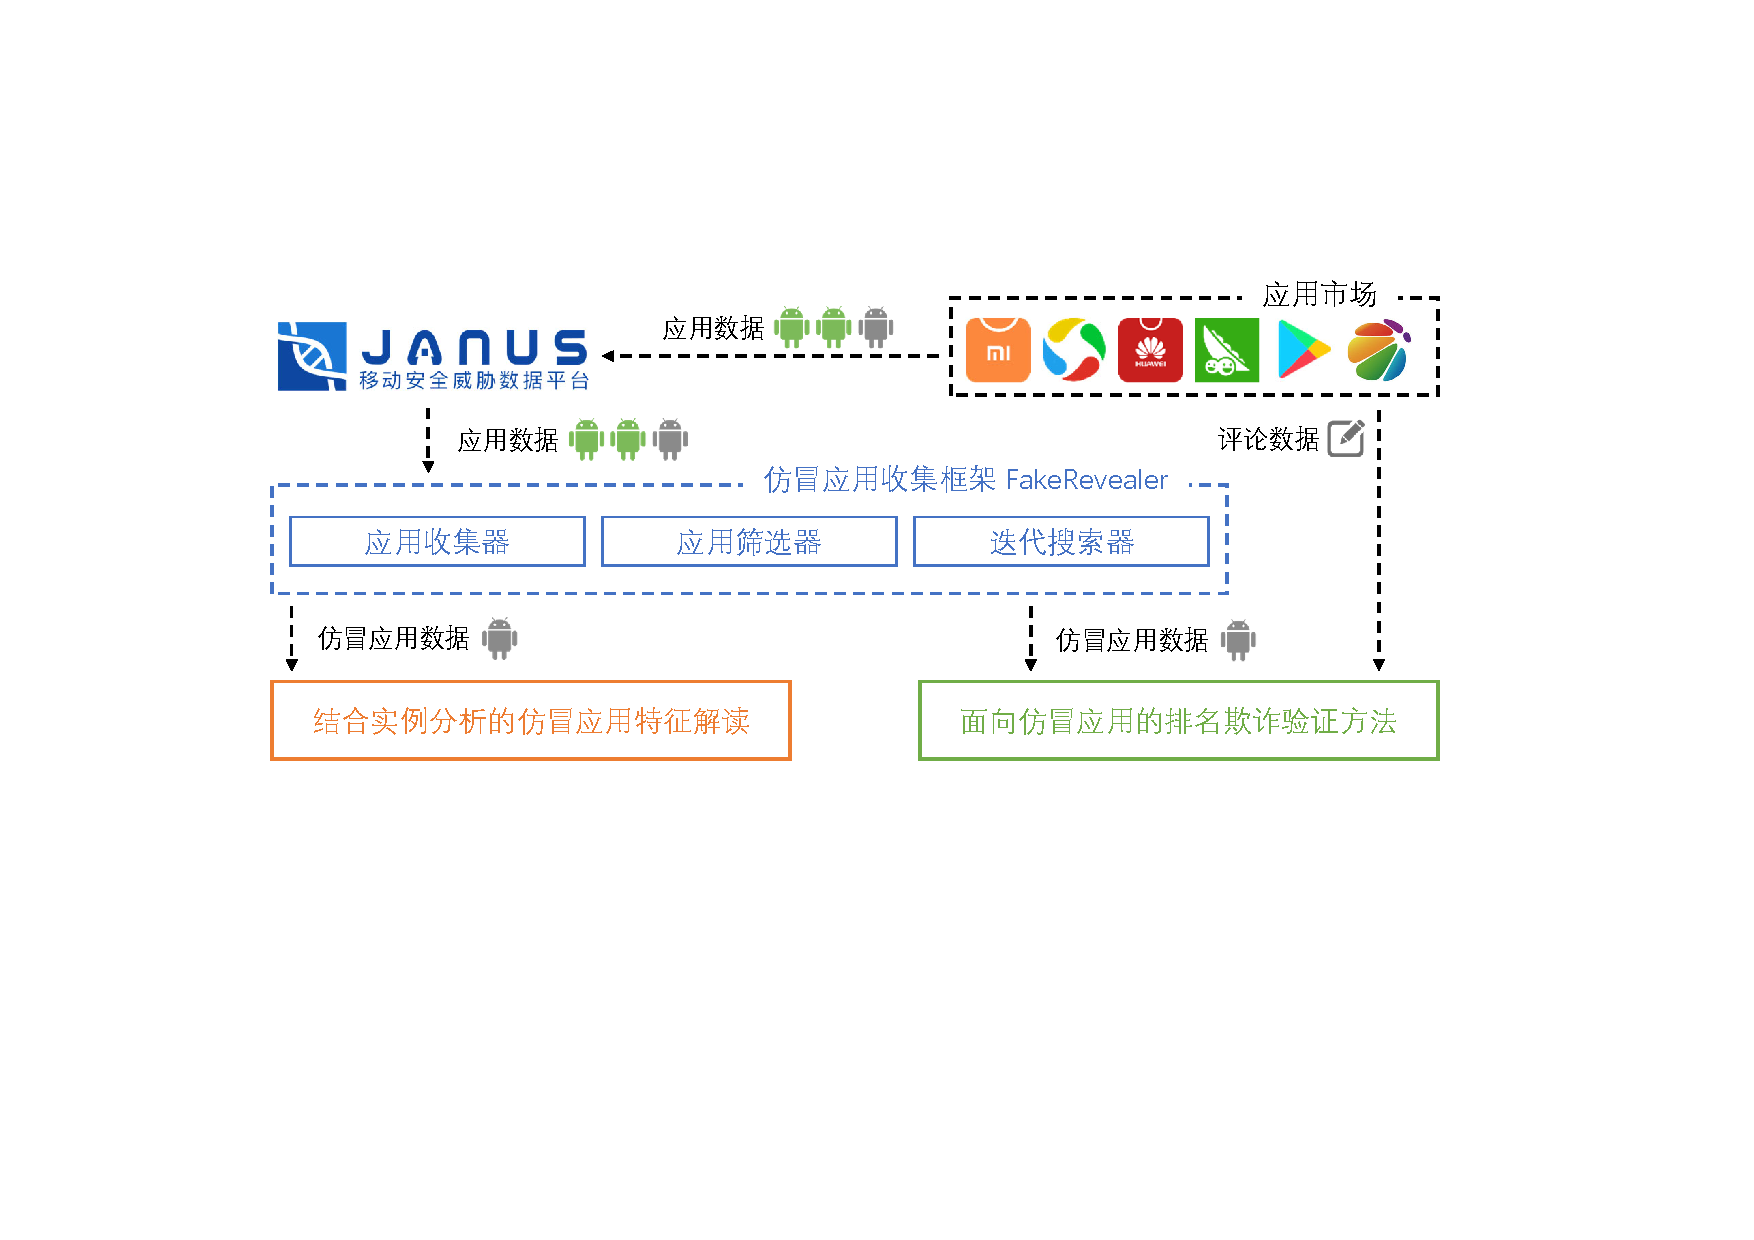
\includegraphics[width=\textwidth]{./Figures/edwin-overview}
% 	\caption{本文工作概览}
% 	\label{fig:Workflow}
% 	\vspace{-3mm}
% \end{figure}
%
% 本节为本文工作提供概览。如\autoref{fig:Workflow}所示,本工作通过三个主要部分,完成三部分工作:
%
% 1)\ \emph{利用面向仿冒应用的收集框架\mytool 收集大规模数据,解决仿冒应用数据稀缺的问题} \quad
% 针对实证研究中实验数据应尽可能具有完整性与代表性的要求,本研究设计并实现了仿冒应用收集框架\mytool,尽可能全面地进行仿冒应用的数据收集。
% 数据收集主要分为两个部分:正版应用信息的收集和仿冒应用的收集。
% 在正版应用信息收集的部分,本文选择了50个最热门的App作为目标应用,然后手动收集了跟这些App有关的信息;
% 基于该50款目标应用,本研究利用\mytool,收集了从29个应用来源获得的近14万个应用样本,并从中筛选出5万个仿冒应用,整理成集。
% 该数据集可为后续相关工作如代码分析、特征检测等提供数据支持。
%
% 2)\ \emph{首次针对仿冒应用的特性进行大规模的特征解读} \quad
% 针对移动黑灰产研究中关于仿冒应用的研究空白,本研究利用上述仿冒应用数据,结合案例分析,进行了首次基于Android系统仿冒应用的大规模特征解读。
% 特征解读从三个视角完成,这些视角分别是仿冒的基本应用特征、影响仿冒应用数量的因素和仿冒应用的发展轨迹,由浅入深揭示仿冒应用的生态。
% 对应的三个案例分析除了为特征解读提供案例支持之外,还揭示了更多仿冒应用开发者的行为特征,可为用户、应用市场和安全领域从业人员等多方受众提供一定见解。
%
% 3)\ \emph{面向仿冒应用的排名欺诈验证} \quad
% 该部分中,本文从第三方应用市场中随机选取一部分应用,爬取用户对它们的所有历史评价,以检测仿冒应用与排名欺诈行为的关联。
% 针对前人检测研究需要先验知识或特殊数据的问题,本研究从社交媒体研究引入了用户行为可信度进行排查,避开了现有方法的局限性。
% 进一步地,本研究从评论内容重复率方面提出了另一创新性排查方法,解决了数据量增大带来的大运算量问题。
% 人工复查结果显示,两种排查方法均取得了优于现有方法的结果。
\section{本文组织结构}
% todo: 7 chapters?
本文共分为七章,环绕着本研究的数据搜集和不同的分析方向展开,各章节内容如下:

\fullref{chp:intro} 主要提供了本文的研究背景、相关工作、本文拟采用的研究方法、拟解决的问题与本文的主要工作。

\fullref{chp:background} 介绍相关技术背景,从软件工程领域的实证研究出发,介绍实证研究的常用方法和数据收集、验证标准等理论背景,再着眼于本研究的主体——Android应用,介绍了Android安全证书机制和与仿冒应用相关的重打包技术。

\fullref{chp:research_settings} 介绍整个研究的设置,包括根据研究现状提出研究问题、确立研究对象,阐述数据收集的相关考量,并与其他研究收集的数据进行对比。

\fullref{chp:discoveries_basic} 从仿冒应用与原版应用相似度、影响应用被仿冒的严重程度的因素及仿冒应用行为三点入手,对与仿冒应用基本特征相关的三个方面进行实证研究,最后针对研究结果分别向用户、应用市场和应用开发者提供实用建议。

\fullref{chp:discoveries_behavior} 则结合应用证书视角与结合时间维度视角进行探索,分析现有应用市场监管策略存在的不足,针对性地提出改善措施。

\fullref{chp:framework_prototype} 提出了一个基于规则的仿冒应用检测框架,并将前两章实证研究所得的经验总结为规则,对框架进行了有效性检验。

% % 这些视角包括仿冒应用特征、影响仿冒应用数量的因素和仿冒应用的发展轨迹,每个视角都被进一步分解成多个不同的研究问题。
% % 说明仿冒应用的数据收集方式并详细介绍其中三个组件(\componentA、\componentB 和\componentC)的设计与实现,
% % 结束解读后,本文从数据中挑选三个具有代表性的案例进行分析,以案例进一步深化分析结果。

% \fullref{chp:feedback} 针对仿冒应用进行了排名欺诈检测。
% 针对现有检测方法的不足,本文先后提出两个具有创新性的方法对排名欺诈行为进行排查,并将排查结果与前一章的仿冒应用进行比对。
% % 结果显示,仿冒应用存在排名欺诈行为。仿冒应用与排名欺诈行为作为移动黑灰产的两个环节存在关联。

\fullref{chp:future} 对本文工作进行总结,并对下一步工作进行展望。

\clearPaperPage

\chapter{Android背景介绍}
\label{chp:background}

本章主要介绍Android系统、Android应用程序和应用市场相关的背景知识,包括现有的Google Play市场和多个第三方市场共存的局面介绍,同时也会介绍Android安全证书机制的相关背景。

\section{Android系统介绍}
Android系统是属于Google公司的开源操作系统,基于Linux内核研发。
其最早版本于2008年发布(Android 1.0),起先只针对手机端发布。
由于具有图形化操作界面,并且采用触屏作为交互方式,极其简单易用,Android系统自发布起就迅速在智能手机领域抢占大量市场份额,搭载Android系统的平板电脑也在我们的日常生活中渐渐变得随处可见。
近年来,随着IoT(Internet of Things,物联网)的发展,家用电器趋向智能化,不少电视厂商、机顶盒厂商、甚至可穿戴设备厂商也开始为产品内嵌深度定制的Android系统,为用户提供更好的体验。

\begin{figure}[htbp]
	\centering
	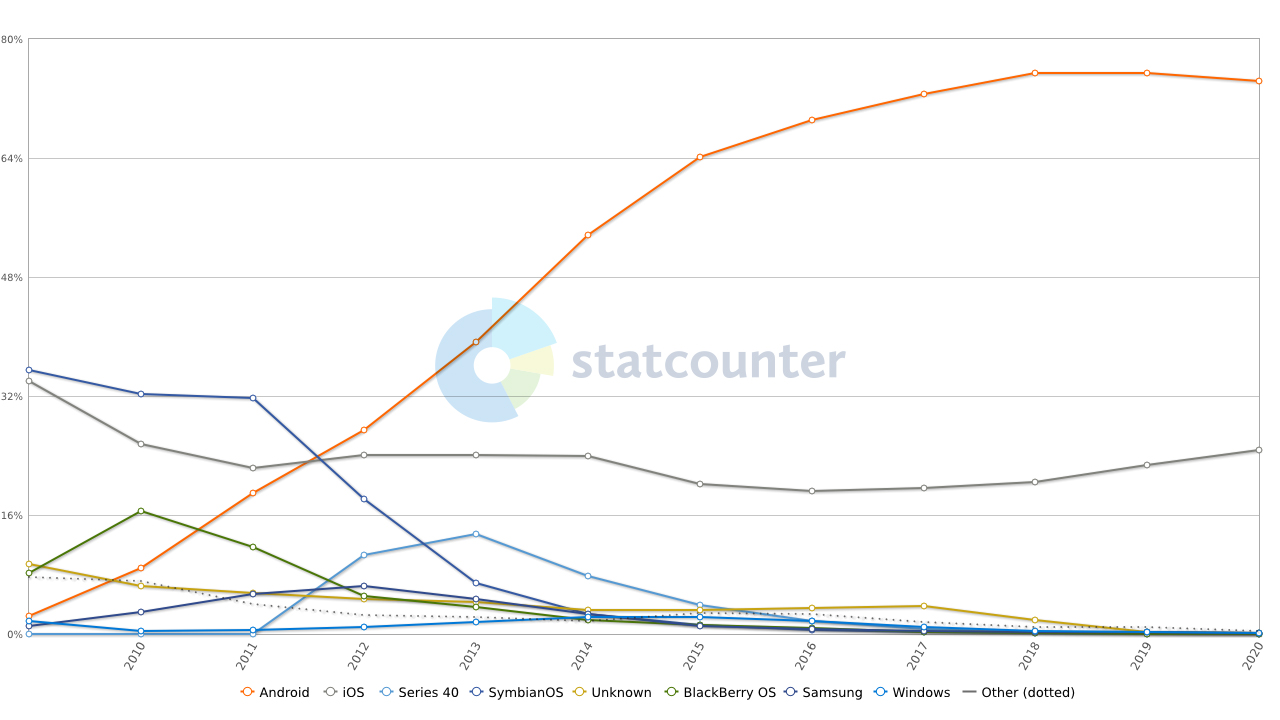
\includegraphics[width=0.95\textwidth]{./Figures/edwin-StatCounter-os-mkt-share-yearly-2009-2020.jpg}
	\caption{2009至2020年移动端操作系统市场份额变化图}
	\label{fig:Android-Mkt-Share}
	\vspace{-5mm}
\end{figure}

图~\ref{fig:Android-Mkt-Share}展现了2009年到2020年间不同移动端操作系统对市场占有率的变化曲线,图表来源于数据分析机构StatCounter~\cite{MobileOSMktShare},图表X轴为时间线,Y轴为市场份额占总量的百分比。
不同颜色的曲线代表不同操作系统,其中Android系统由橘红色曲线表示。
从图中数据可知,自发布以来,Android系统便一路高歌猛进,迅速占据移动端操作系统市场,从2012年起就获得了业界第一的市场份额占有率,直到2020年,其超过70\%的市场占有率依然遥遥领先于其他操作系统。
其中原因,除了对用户非常友好的操作方式以外,也在于其具有一个多元、开放又充满活力的应用程序生态环境。

\section{Android应用程序}

\subsection{应用程序简介}

Android应用程序(Android Application,简称App)是可以安装在Android系统上、拓展系统功能的软件,这些软件通常基于Java语言开发,其中可以包含用C语言或者C++编写的库以提高性能。
2014年起,Google宣布Android支持Kotlin编程语言,自此开发者也可以使用Kotlin语言进行Android App开发。

Android App的开发需要使用Google提供的软件开发工具包(Software Develop Kit,简称SDK)和Google支持的集成开发环境(Integrated Development Environment,简称IDE)。
SDK是包含了众多软件包的工具箱,其中有包括了Android系统应用程序接口(Application Programming Interface,简称API)的函数库和用以编译App的各种工具,在编译完成之后,开发者还可以利用SDK的相应工具为App签上自己的数字签名。
API函数库提供了Android系统的一系列接口,开发者需要在使用Android App框架的前提下,调用各种API实现自己设计的功能。

在发布每一版本Android系统的同时,Google公司也会发布一个新版本的Android SDK供开发者开发App。
每个人都可以从Android的官方网站上下载Android SDK和开发应用所需的IDE,这意味着,利用官方发布的工具,任何人都可以开发出属于自己的Android App。

\subsection{构建应用程序}

与大部分软件一样,开发者在发布自己的App之前,也先需要把代码编译打包成Android操作系统使用的一种应用程序包格式文件APK(Android application package)。
每个APK文件都会包含该款App的一系列基本信息,包括App的应用名、包名(Package name)、安全证书等。
其中,包名是Android系统识别App的依据,每款App在不同的版本可以有不同的应用名,但其包名必须是一致的。
图~\ref{fig:Android-Build-Process}展现了APK文件的构建流程。
一般来说,一个Android App的构建流程会分为以下四步,整个构建流程由Android SDK中的Android插件和Gradle构建工具管理。

\begin{figure}[htbp]
	\centering
	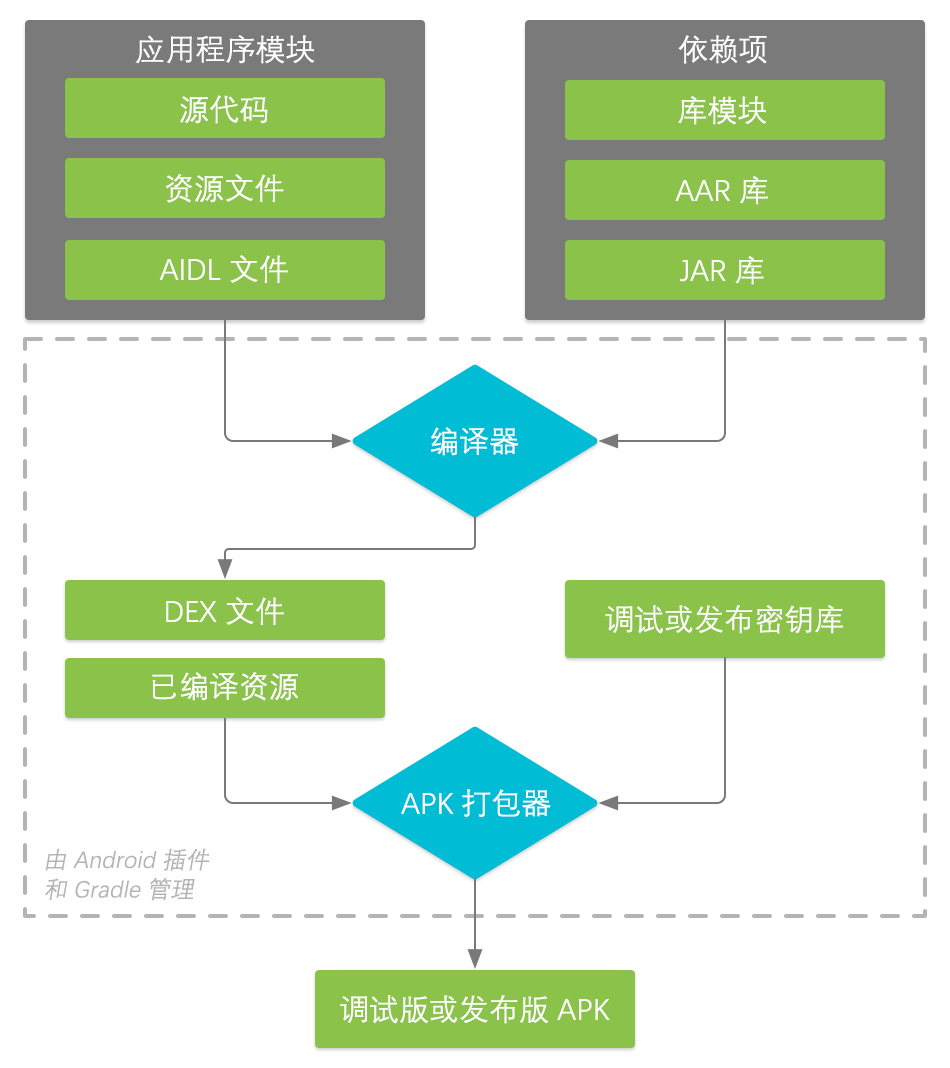
\includegraphics[width=0.6\textwidth]{./Figures/edwin-build-process-CHN.png}
	\caption{Android App构建流程}
	\label{fig:Android-Build-Process}
\end{figure}

首先,开发者需要编写App对应的源代码,然后连同一些源代码中使用到的依赖项一起输入到编译器中生成DEX文件。
源代码可以由Java语言或者Kotlin语言编写,而DEX文件则是一种可执行文件,可以运行于Dalvik虚拟机上。
Dalvik虚拟机则是Android系统的核心组成部分之一,用于运行被编译为DEX文件的程序。
此外,编译器还会将其他未被编译的资源文件转换为编译后的资源。

然后,SDK中的APK打包器会将DEX文件和已经编译好的资源文件一起打包。
APK文件的本质是压缩文件,其中包含了被编译的代码文件、App需要用到的资源文件(比如字符串、图片等资源)、assets资源、App的安全证书和Manifest配置文件,所以APK打包器的任务是将这些所有文件都压缩进一个APK文件里面。
不过,在这个步骤,APK打包器还未将所有文件压缩。
因为在压缩之前,还需要进行下一步的签名。

在第三步,APK打包器会使用密钥库文件对上一步中提及的资源文件和代码文件进行数字签名。
这个步骤是用作校验APK文件是否被篡改、保证APK文件完整性的一个重要步骤,在本章后续内容中会有相关机制的更多介绍。

最后,APK打包器会使用zipalign工具对应用进行优化,以减少App在设备上运行时所占用的内存。
这步结束之后,整个构建流程也随之结束。
开发者会获得一个编译好、签名完毕并且经过优化的APK压缩文件,然后就可以将这个APK文件安装到Android设备上运行使用。


\section{Android应用市场}
由于每个人都可以开发、构建自己的Android App,从网上发布的App数不胜数。这种开放性为Android应用生态带来开放性的同时,也会引入以下几个问题:

1)\ \emph{难以择优} \quad
开放的环境会导致App数量难以胜数。由于从互联网上找到的App质量良莠不齐,用户有时无法判断网上的应用是否符合自己的需求;

2)\ \emph{数据安全} \quad
智能手机与现代人的日常生活息息相关,其中也自然包含了各人的隐私数据甚至财产信息。确保用户下载、安装到的应用不会损害到他们的财产安全和数据安全至关重要;

3)\ \emph{宣传渠道} \quad
开发者希望自己的App尽可能地受欢迎,但中小开发者并没有足够的资源去宣传自己的应用,可能会导致原本质量优秀的App因为缺少宣传渠道而无人问津;

4)\ \emph{收入结算} \quad
开发者有从App中获得盈利的需求。即使是部分出于兴趣或其他非盈利目的开发手机应用的开发者,也需要从App中获取补贴以维持App的维护和正常运作。如何利用App变现、变现之后又要怎样将资金回流到开发者的问题有待解决;

5)\ \emph{应用更新} \quad
随着时间推进,用户的需求并非一成不变,开发者也需要针对App中以往出现的漏洞查漏补缺、或者更新软件功能,但要求用户定期/不定期地手动更新某个App甚至多个App并不现实。

Google发布的应用商店Google Play~\cite{GooglePlay}的存在缓解了以上的问题。它是Android操作系统的官方应用商店,可以让用户浏览和下载商店中的App。
一方面,普通用户可以经由Android系统中预装好的Google Play服务寻找、购买和下载心仪的App;另一方面,Google Play也允许开发者将App通过开发者账户上传到Google Play中,在经过一系列的审查之后上架到商场上供用户下载。与上述的五个问题对应,Google Play应用商店提供了以下几点服务:

1)\ \emph{一个由官方背书的下载渠道} \quad
这确保了用户下载的App得到官方认可。同时,Google Play也提供了一个关于App的社区条件,用户可以对App进行打分、评论,用户对App的评价经审核后可以由所有其他用户查看,直接影响其他用户对``是否要下载某款应用''的决定;

2)\ \emph{上架之前的应用审核} \quad
在开发者上传App时对App作出一定的审查,以排除部分恶意开发者在商场中上架病毒和恶意应用的可能性。Google Play也会根据用户反馈、应用本身运营数据等原因于每季度从商店中移除一部分App,以保证商店货架上App的质量;

3)\ \emph{作为激励机制的推荐榜单} \quad
在用户评价的基础上,Google Play筛选出一部分质量优异的App制订出一些推荐榜单。推荐榜单会在应用商店首页进行展示,榜单包括``编辑精选''、``热门应用''、``年度之选''等,其中既有大公司开发的App,也会有中小开发者独立开发的应用。此外,Google还会通过用户的使用习惯、所在地区等因素为用户提供个性化推荐(如图~\ref{fig:Google-Play-Main}所示),在不同的App类别下,也有不同榜单为用户推荐,加大了优秀App的曝光率;

\begin{figure}[htbp]
	\centering
	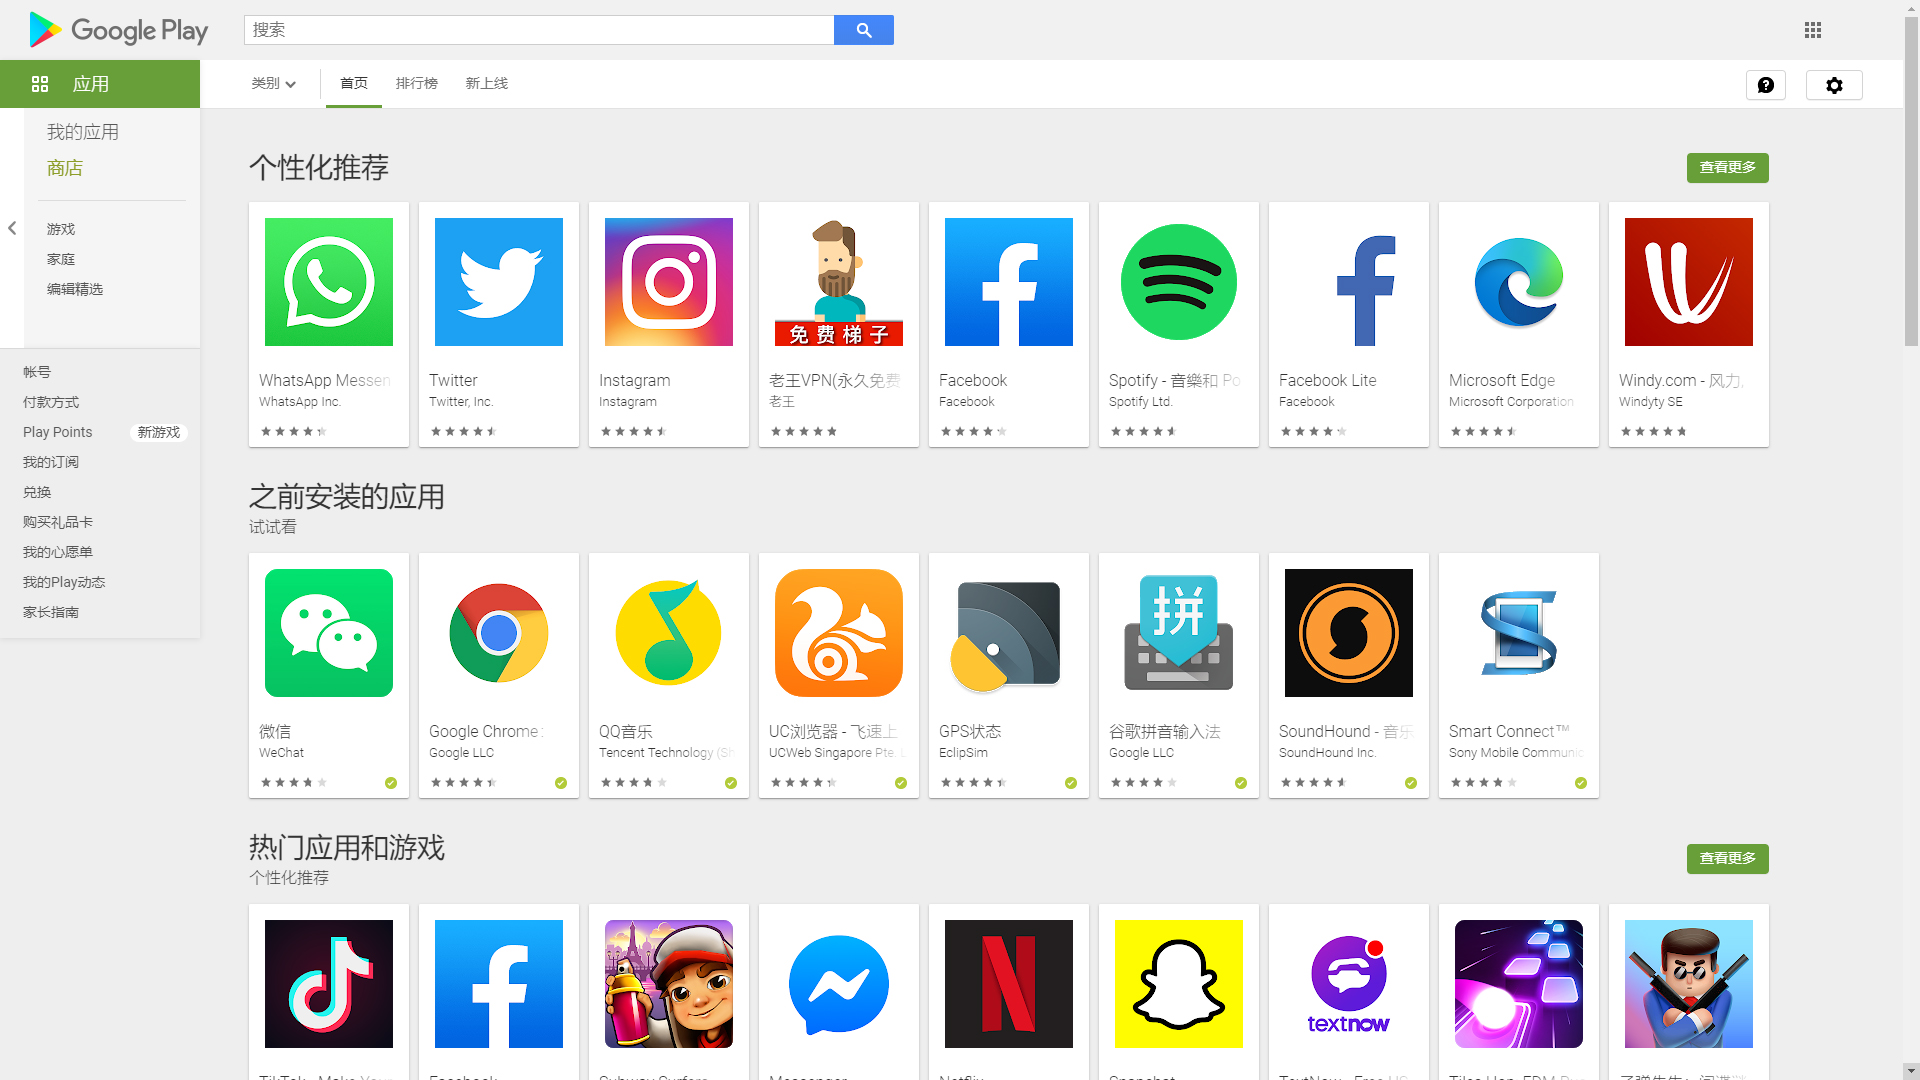
\includegraphics[width=\textwidth]{./Figures/edwin-google-play.jpg}
	\caption{Google Play应用商店首页(从桌面端浏览)}
	\label{fig:Google-Play-Main}
\end{figure}

4)\ \emph{集中的结算通道} \quad
Google Play应用商店为开发者提供了一个统一的结算渠道。应用开发者可以在App内销售商品,然后选择Google Play提供的集成结算服务。用户在购买服务时,直接向Google付款,Google再在每个结算周期将款项结算给开发者。这样一来,开发者尤其是独立开发者就可以更专注于App本身的开发,而不需要考虑如何利用应用变现、再将资金回收的复杂问题。Google Play也允许开发者将自己的App上架为付费应用,需要用户付款后才可下载;

5)\ \emph{方便快捷的更新推送} \quad
由于Google Play本身是个应用程序的集中平台,而且也预置到了大多搭载Android的设备中,所以开发者在更新应用时,只需将新版本上传到Google Play的后台,应用商店经过审核之后,就可以将新版本的应用推送到用户的设备中,让用户设备中的App实现自动更新,免去双方的麻烦。


\section{第三方应用市场}

Google Play应用商店无疑为用户和开发者都提供了一个优良的解决方案,每个应用底下由用户评论组成的社区也促成了用户和开发者之间的交流,用户反馈直接推动了开发者对应用的改良。

遗憾的是,由于种种原因,Google Play应用商店的服务并非对全球的所有地区和国家都开放。
Google从2008年开始退出中国大陆市场,因此Google的大部分服务,包括Google Play应用商店的下载服务在内,都不向中国大陆境内用户提供。
换句话说,国内的大部分普通用户并不能享受到Google Play应用商店的便利。

为此,国内有多家厂商都推出了自己开发的应用市场服务,试图填补这一片市场空白。
实际上,由于整合开发者、用户和App资源三者本身就有巨大的市场潜力,所以即使是在Google Play服务可用的其他国家和地区,也有厂商推出自己的应用市场(如三星推出的三星应用商店、Amazon推出的Amazon应用市场),试着在这个市场上分一杯羹。

纵观国内的应用市场,经过几年的竞争与整合,依然未有出现像Google Play应用商店一样具有垄断性地位的厂商。
多个厂商各据一方,主要可以分为两个类别。
一类是国内IT行业巨头旗下的应用市场,如腾讯旗下的应用宝~\cite{Myapp}和百度旗下的百度应用市场~\cite{Baiduappstore},其平台本身就具有大量基础用户,可以直接转化为应用市场中的活跃用户;另一类则是由各大手机厂商开发的应用市场,如华为的应用市场、小米的小米应用市场~\cite{Xiaomiappstore}等,这类的应用市场通常直接预装在手机出厂时自带的厂家定制Android系统中,凭借手机销量直接带动市场用户增长。

根据数据分析机构艾媒咨询于2018年12月发布的《2018-2019中国中国移动应用商店市场监测报告》~\cite{ChineseAppStoreReport}显示,使用第三方移动应用商店的用户在手机网民中占比为59.99\%。结合国内网民数目庞大的现状,这一数字表示第三方应用市场在国内已被广泛接受。而40.01\%未使用第三方移动应用商店的用户比例则表示这一市场还有广阔前景。该报告还提供了2018年国内第三方应用市场用户首选市场的分布图,如图~\ref{fig:CHN-Mkt-Dist}所示,用户对第三方移动应用市场的选择主要还是集中在国内IT巨头发布的应用市场上。约40\%的手机用户会使用360旗下的360手机助手作为首选应用市场,而首选使用豌豆荚、UC应用商店等阿里应用分发平台旗下应用商店的用户约占11\%。大部分市场份额都已被国内IT巨头旗下的应用市场占领。

\begin{figure}[htbp]
	\centering
	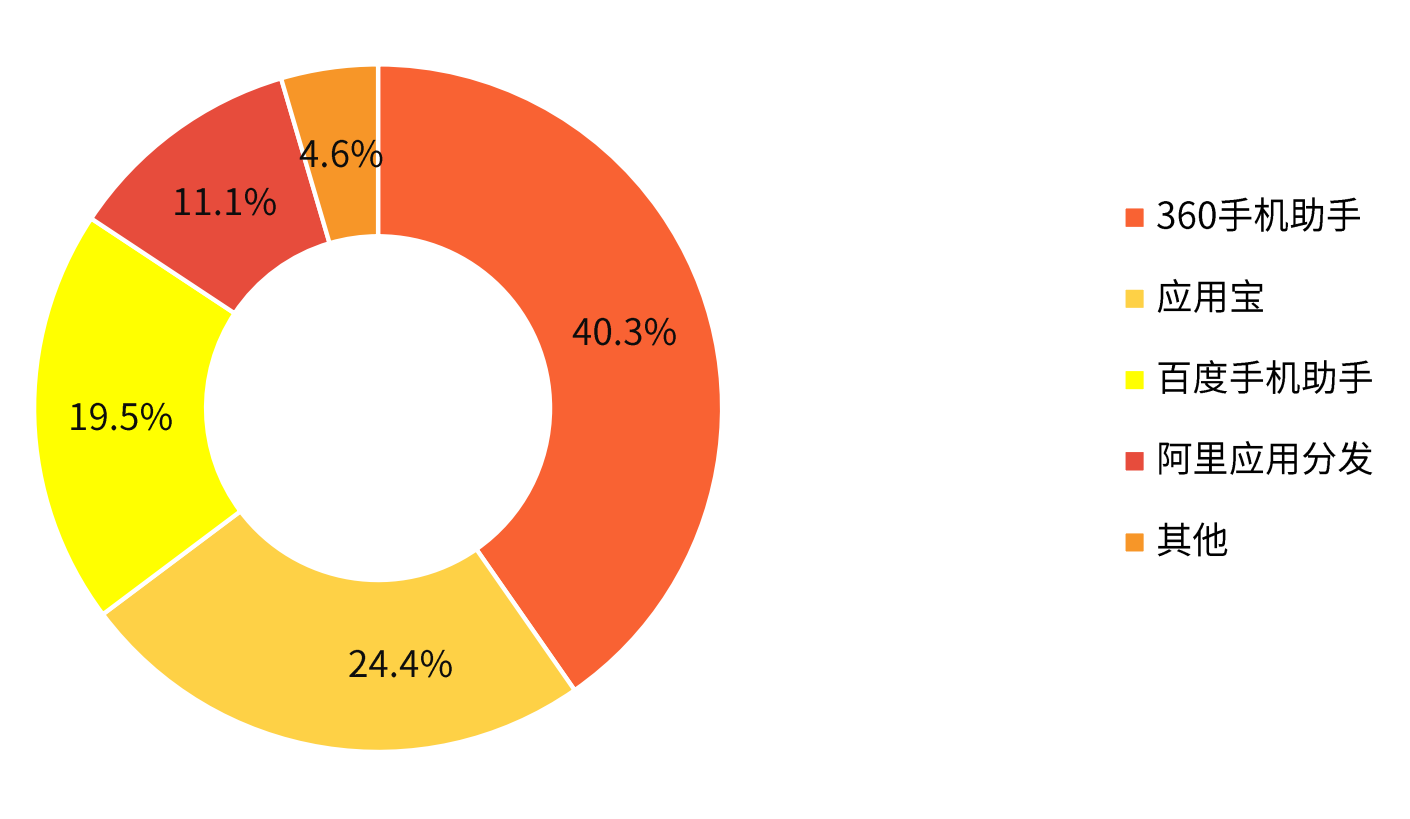
\includegraphics[width=0.5\textwidth]{./Figures/edwin-CHN-mkt-dist.png}
	\caption{2018中国第三方移动应用商店用户首选使用品牌分布}
	\label{fig:CHN-Mkt-Dist}
\end{figure}

与Google Play提供一个完整的Android生态环境相似,上述的各个厂商也致力于构建各自的Android应用生态链条:各大厂商本身就具有一定知名度,从其旗下的应用市场下载应用能让用户放心;开放开发者中心,让开发者注册账号后上传自己制作的App;为每一个App提供评分和评论功能,构建出开发者和用户的交流平台;在应用市场首页设置应用排行榜、推荐安装软件等榜单(如图~\ref{fig:mkt-yyb}),提高优秀App的曝光率;应用市场自带的应用版本管理开发者在市场后台更新应用之后,将更新推送到用户的手机上;各大应用市场也会整合支付平台(如支付宝和微信支付)来应对市场内的应用购买业务,华为应用市场甚至像Google Play一样,为市场上的应用提供了自家的支付渠道以支持应用内的付款项目购买功能。

\begin{figure}[htbp]
	\centering
	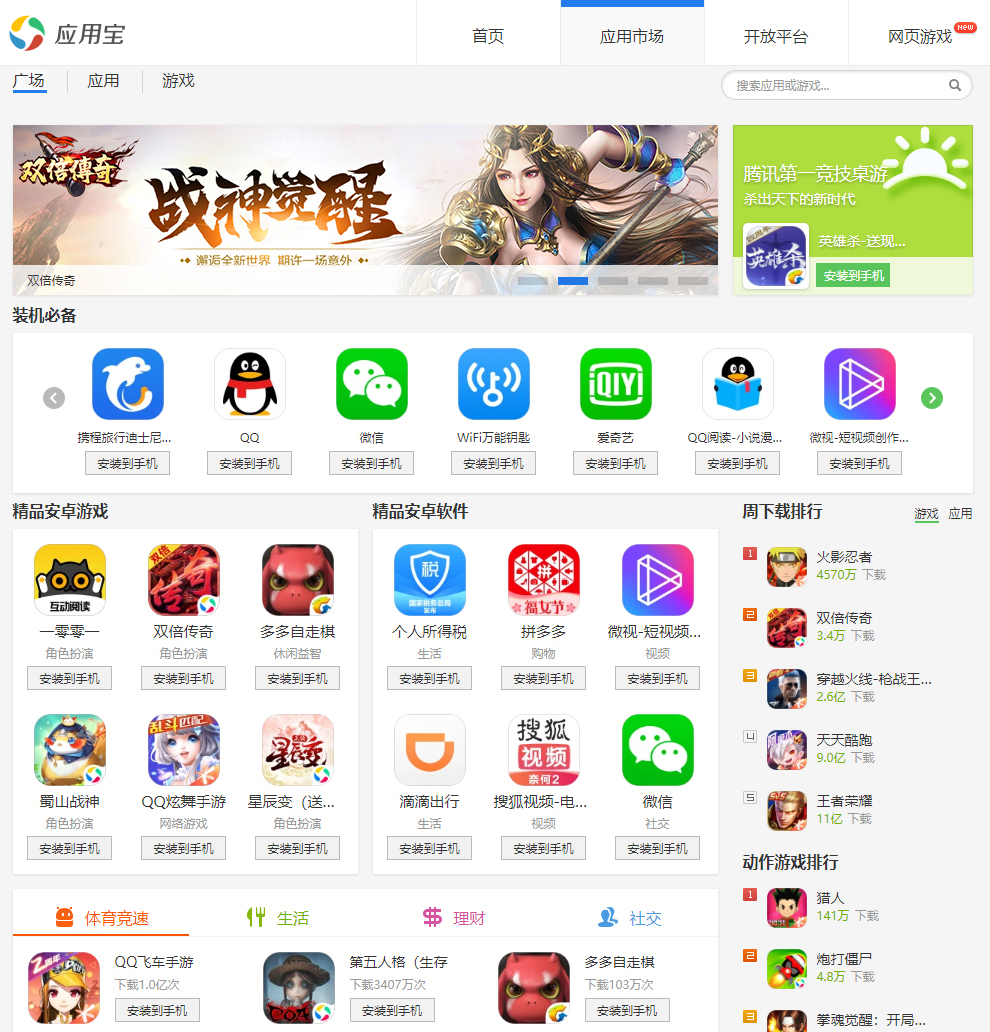
\includegraphics[width=0.8\textwidth]{./Figures/edwin-yyb.jpg}
	\caption{腾讯应用宝应用市场首页(从桌面端浏览)}
	\label{fig:mkt-yyb}
	\vspace{-5mm}
\end{figure}

不同于在Android系统发布早期就存在的Google Play应用商店,国内的第三方应用商店是后期出现的产物,一出现就面临着激烈的市场竞争。
一方面,在国内各类第三方应用市场方兴未艾之时,国内的Android开发者社群尚未成熟,应用市场还未有大量开发者进驻;
另一方面,在成立初期,为了抢占市场份额,各个应用商店都想方设法将商店内App的种类和数量最大化,以迎合市场用户各种各样的需求。
作为结果,各类第三方应用市场都在各个渠道搜集App,而非通过开发者上传的方式获得货架上的应用程序。
由于在早期各种监管渠道尚未完善,各个市场在搜罗各类App的同时,难免会将大量的盗版应用也一并收录。

\section{Android App签名机制}

前文提到,开发者在使用Android SDK构建App时,其中十分重要的一步是对App进行数字签名。
实际上,Android的数字签名和安全证书机制基于RSA公共密钥系统,是Android安全机制中不可或缺的一个部分。
本章的余下内容将会对Android App的签名机制进行简单分析。

Android App的签名机制是用作校验APK文件是否被篡改、保证APK文件完整性的一个重要机制,所有的应用都必须要在经过签名才能安装进Android系统中。
在签名时,SDK会使用一种密钥库文件,如果开发者还没有这个文件的话,SDK会自动生成一个。
密钥库中包含了开发者的各种信息,包括一对公钥和私钥。
私钥用于数字签名,不可向外公布;公钥则是可以向外公布的一组密钥,用于数字前面的验证。
App中的签名也是系统用来识别开发者的重要依据,因为同一个密钥库文件会产生一致的签名,系统能根据签名中的公钥验证应用识别开发者。

签名的过程大致如下:
在前文流程的第二步结束后,编译器会输出DEX文件和编译好的资源文件,这时,SDK会对每个文件都扫描一次,然后对每个文件提取一次数字摘要,再把每个文件的文件名和其对应的数字摘要保存在一个名为\textit{MANIFEST.MF}的文件中。
之后,SDK会再扫描一次刚才生成的\textit{MANIFEST.MF}文件,再次提取一次数字摘要,把这个摘要连同刚才文件中的所有内容存入另一个新文件\textit{CERT.SF}里。
第三步,再计算一次\textit{CERT.SF}的数字摘要,然后用密钥库中的私钥对这个摘要进行加密。
加密后的结果就是数字签名。
最后,SDK将签名、公钥、计算数字摘要的哈希算法等信息写入\textit{CERT.RSA}文件中,再将这整个过程中生成的四个文件放进\textit{META-INF}文件夹,用APK打包器打包起来。
至此流程结束。

而Android系统验证签名的方式,则是先通过\textit{CERT.RSA}中的公钥验证签名是否无误,再根据文件中提供的哈希算法计算APK包中所有文件的数字摘要:先从\textit{CERT.SF}开始,然后是\textit{MANIFEST.MF},然后是APK中的其他所有文件...
一旦其中出现不相符的结果,就会导致验证失败。
在安装App的过程中,验证签名失败会使得系统终止App的安装。

换句话说,在一个APK被打包签名完毕之后,如果需要更改其中的内容,就只能在更改后将APK重新打包签名一次,即使是一个bit的修改也会破坏原有的签名。
这也是系统可以用数字签名识别开发者的原因:签名一致的App,最后一定都是由同一个开发者打包的。
所以,具有同样签名的App也可以在同一个Android设备上共享数据。
不过这超出了本文讨论的内容,故按下不表。

目前,签名的模式共有三代,其区别主要在于构建流程第三、第四步之间的一些操作上。
简单地说,越新的签名模式能越好地保障APK文件的完整性。
实际上,第一代签名模式V1具有较为致命的缺陷,所以Google官方也在呼吁开发者在编译时采用最新的签名模式。

要注意的是,签名机制只能保证APK文件在被篡改之后不能凭借原有的签名被安装进Android系统,但恶意开发者依然可以在篡改APK之后,用自己的密钥库对APK重新签名,构建出可安装的App。
这种App是盗版App的一种,被称为重打包App。

\section{本章小结}

本章主要介绍了Android系统、Android应用和Android应用市场的相关背景知识,同时也阐述了Android应用的构建流程和简要介绍了其中使用到的签名机制,为后文实证研究中使用到的采样来源和验证方法做铺垫。

\clearPaperPage

% \chapter{面向仿冒应用的收集框架\mytool}
\label{chp:fakerevealer}

\section{设计缘由}
鉴于目前学术界中未有相关工作能提供仿冒应用的相关数据集,本研究需要率先尝试从工业界中系统地收集所需的仿冒应用数据。
然而,传统的网络爬虫框架只能机械、不加区分地爬取数据,不能具有针对性地爬取与本研究中的目标应用相关的样本;应用市场中应用数量太多,完全收集并不可行。
为了解决这个问题,本研究提出了面向仿冒应用的收集框架\mytool,创新地采用启发式的方法搜索与爬取与目标应用相关的样本,为后文的两项研究服务。

\section{应用收集流程简介}
仿冒应用是一个跟正版应用相对的概念,所以本文需要先定义正版应用,再根据正版应用的信息搜寻仿冒应用。

1)\ \emph{正版应用收集} \quad
在定义正版应用方面,本研究参考了数据平台易观千帆的月度App排行榜~\cite{yiguanqianfan},然后从中选出了其中的前50款热门App作为本次研究的目标应用。
之后,本研究逐一地从这50款App的官方网站上下载了这些应用的最新版本,作为正版应用的参考版本。

2)\ \emph{仿冒应用收集} \quad
要获取足量的仿冒应用数据以组成数据集是一个十分具有挑战性的任务,难点如下:
\begin{itemize}
	\item 要从多个不同的应用市场中爬取App样本,但每个应用市场都有不同的网页编码,不存在一个爬虫脚本对所有应用市场数据都通用的场景;
	\item 各个应用市场架上的App数量浩如繁星,需要有效地找到和目标应用有关的所有样本,不重不漏;
	\item 对于大量数据,需要一个轻量级的解决方案快速判断获得的App样本究竟为正版应用又或者是仿冒应用。
\end{itemize}

为了应对第一个挑战,本研究与工业界合作,利用犇众信息公司的Janus平台对各大应用商店进行样本爬取,从而获得大量应用样本。
事实上,如\autoref{fig:Janus-data}显示,Janus平台自2017年起就开始对各大应用商店的App进行样本收集,至今已收集到上千万个App样本。
除样本搜集外,Janus也提供按规则搜索功能,用户可以创建自己的规则过滤平台中的应用数据,以获取自己需要的App样本。

\begin{figure}[htbp]
	\centering
	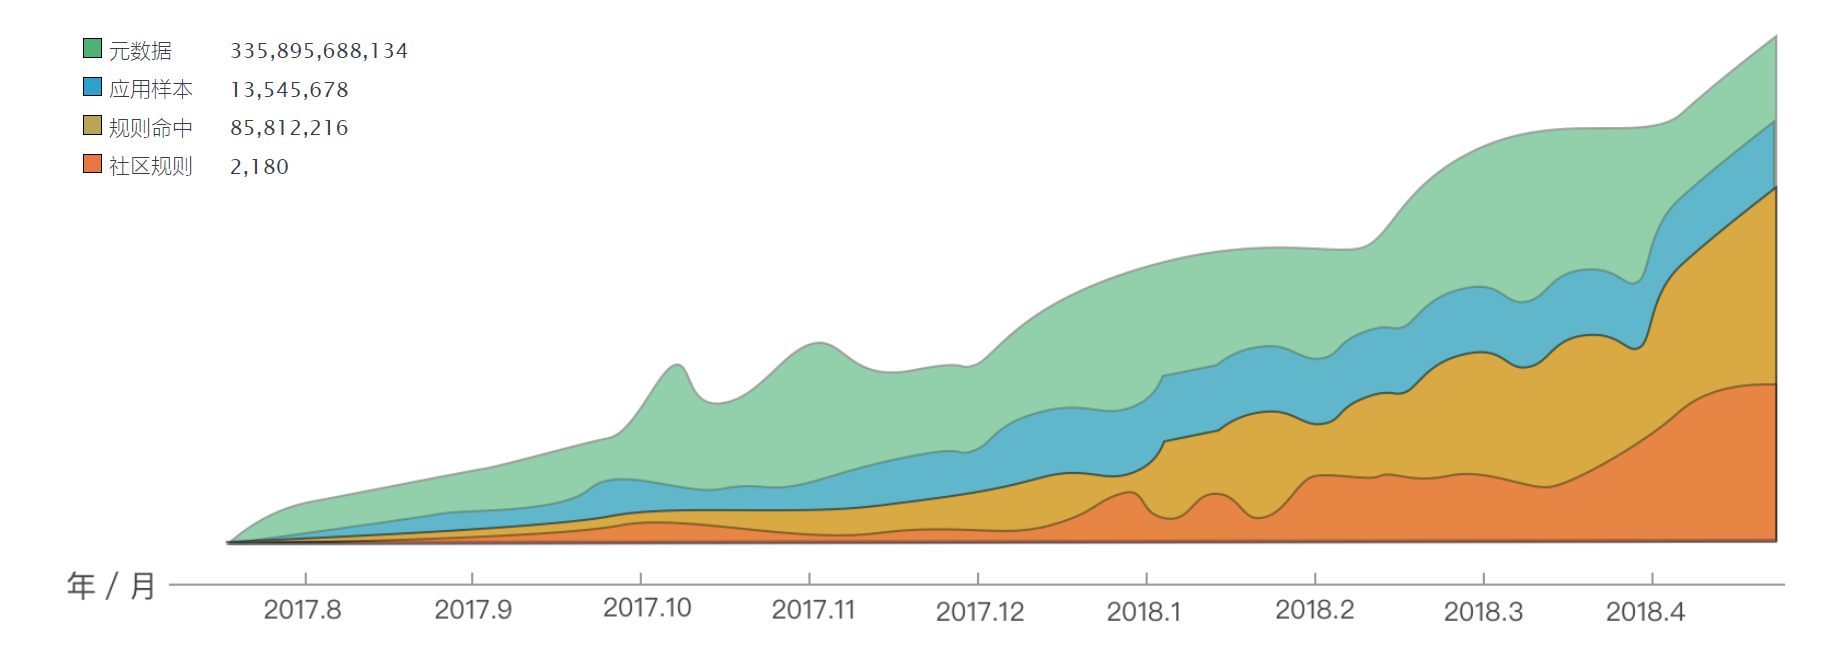
\includegraphics[width=\textwidth]{./Figures/edwin-Janus-data.png}
	\caption{Janus平台上的数据规模时序图}
	\label{fig:Janus-data}
	\vspace{-5mm}
\end{figure}

为了应对第二个和第三个挑战,本研究搭建了面向仿冒应用的收集框架\mytool。


\section{\mytool 的设计与实现}

本文使用Python 3开发了仿冒应用收集框架\mytool,该框架由\componentA 、\componentB 和\componentC 三个组件组成,\autoref{fig:FakeRevealer}展示了\mytool 的整体流程图。
输入初始正版应用的信息,\mytool 在经过迭代搜索、样本下载、应用过滤三个步骤之后,以CSV文件和JSON文件的形式输出仿冒应用各数据项和拓展后的正版应用信息。

\begin{figure}[htbp]
	\centering
	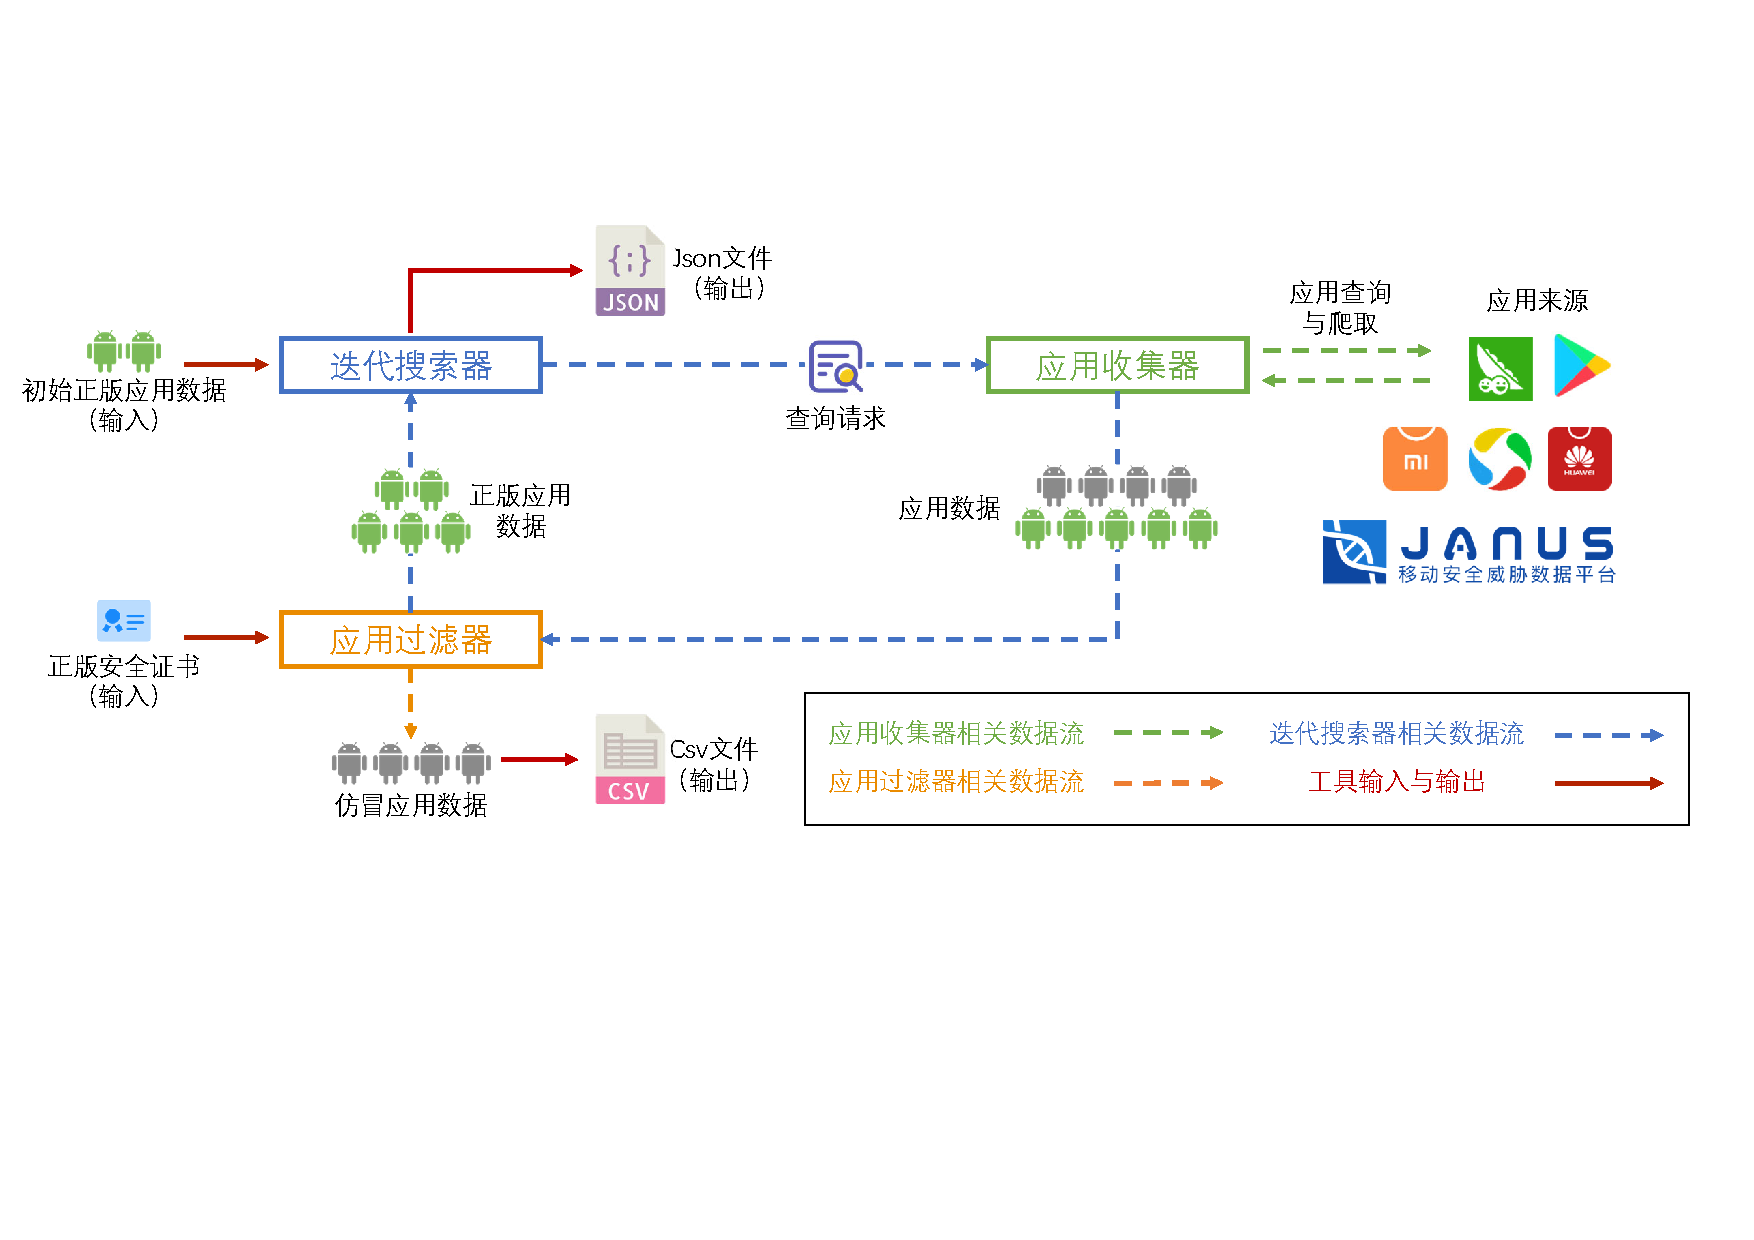
\includegraphics[width=\textwidth]{./Figures/edwin-fakerevealer}
	\caption{\mytool 整体结构}
	\label{fig:FakeRevealer}
	\vspace{-3mm}
\end{figure}

\subsection{\componentA }
\componentA 是与应用来源直接交互的部分,分为两个不同的子模块,分别是网络爬虫模块和APK包预处理模块。
在接收到应用收集请求之后,\componentA 会先根据收集请求,利用网络爬虫模块下载应用,然后再用APK包预处理模块对下载完毕的APK包提取信息,方便后续操作。

1)\ \emph{网络爬虫模块} \quad
本模块负责接收\componentA 的输入,根据输入中的需求从应用来源中查询并下载对应的App。
由于Janus平台上已经有提前收集好的源于各个应用市场的App样本,本研究直接从Janus上爬取应用。

不同应用商店提供应用查询、下载的API不同,不存在可以对应所有应用市场的爬虫脚本。
但只要研究者能分析出某应用商店查询、下载API的名称和用法,结合应用商店账户的Cookies,就能从该商店中下载应用。
考虑到这个方面,本研究设计了插件化的爬虫模块。
针对不同的应用商店,使用者可以在使用网络包分析工具(如Burpsuite~\cite{burpsuite})解析到API与Cookies信息之后,将对应API和Cookies写入配置插件,再对网络爬虫模块配置对应当前商店的插件,开始爬取应用。

在具体实现方面,本研究利用Python自带的urllib库实现对网络资源的访问;由于下载是可以并发进行的事务,为了能提高运行效率,代码实现利用了threading库对网络爬虫模块提供了多线程特性。

2)\ \emph{APK包预处理模块} \quad
这个模块负责从下载完毕的APK包中提取指定的数据项,存入键值对中,最后将所有应用的数据键值对以列表形式返回,作为\componentA 的输出。
APK文件中虽然包含着应用的所有信息,但本研究中的应用筛选并不需要用到整个APK文件,所以本模块会把筛选需要用到的数据先提取出来,后续处理时直接调用与该APK包有关的数据即可。
同时,由于不同APK包的大小不一,所需下载时长也各异,本框架在较大的应用还在下载的同时,对已经下载完毕的APK提取信息。
比起让\componentA 直接返回下载完毕的APK包、待后续需要数据时再进行数据提取的方法,这样的设计可以减小内存占用,也提高了框架的运行效率。

具体实现方面,APK包预处理模块使用Python的os库实现对命令行指令的调用,然后利用Android SDK中自带的命令行工具aapt对APK包进行解析,获取指定的数据项。


\subsection{\componentB }
这个组件的设计利用了一个基于广度优先搜索(Breadth-First Search,简称BFS)的算法,详情可见\autoref{alg:bfs}。
根据缓存中的正版应用信息,本组件向\componentA 提交查询、下载样本的请求。
在利用\componentC 过滤获得的应用信息后,再根据其中正版应用的信息扩增缓存中的数据,进行下一轮迭代搜索。

\begin{algorithm}[!ht]
	\tablewuhao
	\caption{迭代搜索算法}
	\label{alg:bfs}
    \KwIn{ $targetItems$,列表,用于拓展的数据项}
    \KwIn{ $legalApkInfo$,列表,包含正版应用及其信息键值对}
	\KwOut{ $cache$,列表,缓存拓展后的正版应用信息键值对}
	\SetKwProg{Fn}{Function}{:}{}

	\Fn {iterSearcher($legalApkInfo, targetItems$)} {

        $wtQueue$ = $\emptyset$;

        $cache$ = $\emptyset$;

        \For {$apkInfo \in legalApkInfo$} {

            \For {$item \in targetItems$} {

                $wtQueue$.add(${item: apkInfo[item]}$);

            }

        }

    	\While {$wtQueue \ne \emptyset$} {

    		$key, val$ = $wtQueue$.pop();

    		\If{${key: val} \in cache$} {continue;}

    		$cache$.add(${key: val}$);

    		$newSamples \gets$ appRetriever($key, val$);

    		\For {$sample \in newSamples$} {

                $isLegal \gets $ FakeFilter($sample$).getResult();

    			\If {$isLegal$} {

    				$sampleInfo \gets sample$.getInfo();

    				\For {$item \in targetItems$} {

    					$wtQueue$.add(${item: sampleInfo[item]}$);

    				}

    			}

    		}

    	}

    \KwRet{$cache$};

    }

\end{algorithm}

\autoref{alg:bfs}的输入有两项,分别是已有的正版应用信息列表$legalAppInfo$和要用来拓展搜索范围的数据项$targetItems$。

算法开始前,本框架先遍历每个正版应用的信息,将每个要拓展搜索的数据项对应的内容$apkInfo[item]$插入到待查询队列$wtQueue$中,完成初始化(第4 - 6行)。
然后是迭代搜索应用。
每次迭代中,本算法都从$wtQueue$中取出一组键值对,其中键$key$为本次迭代中用于搜索新应用的数据项,$val$为数据项对应的值(第8行)。
取出键值对之后,算法先检查该键值对是否已经被用于之前的搜索中。
如果该键值对之前已经出现过,就跳过本轮迭代,重新取一组键值对进行搜索;
否则,将本组键值对放入数据缓存$cache$,表示该组键值对已被使用过。
之后,组件将键值对传递给\componentA ,\componentA 会生成对应查询,从应用来源中获取数据项相关的应用(第12行)。
对于\componentA 返回的应用集$newSamples$中的每个样本$sample$,本文会用\componentC 检查$sample$是否为正版样本。
如果是正版样本,那么本算法将从该样本中获取对应的数据$sampleInfo$,然后将其中与待拓展对应项$item$对应的内容插入到待查询队列$wtQueue$中(第15 - 18行)。
当应用集$newSamples$中的所有样本都被筛选检查过之后,本轮迭代结束。
如果$wtQueue$中的所有键值对都已经被检索完毕(即$wtQueue$为空),本算法流程结束,本组件会将$cache$中被用于拓展搜索的各个数据项键值对整理成JSON文件输出,方便之后的再利用。

在本次实证研究场景中,$targetItems$包含两项内容,一个是应用的包名(\emph{PackageName}),另一个是应用自身的名字(\emph{AppName})。
之所以要这样操作,是因为开发者推出的App的应用名和包名并不是一成不变的。
一些热门应用会出于商业原因频繁地更改自己的应用名(比如爱奇艺视频,会根据其近期热播的电视剧/电影变更其应用名以吸引更多用户使用);
也有个别的热门应用可能会更换自己的包名,比如App有重大改版、又或者是开发者安全证书有变更,开发者不得不更换包名(具体原因可参考\secref{sec:signature}的Android App签名机制部分)。

\subsection{\componentC }
顾名思义,\componentC 的功能是从输入的应用程序集之中将仿冒应用筛选出来,其核心是安全证书的识别。
根据\secref{sec:signature}中对Android应用签名机制的描述,一个App中包含的安全证书文件指示了对APK文件进行修改的开发者。
如果一个APK文件中包含的安全证书信息与指定应用的开发者信息相符,那么本组件认为这个APK包来源于正版的开发者;否则本组件认为这是一个仿冒应用。

在开始过滤之前,开发者需要先向过滤器导入正版证书信息。
针对上一节提及开发者安全证书可能有变更的情况,本研究仔细排查了所有目标应用,以确保初始化\mytool 时没有正版证书被遗漏。
之后,对于每个输入的应用,组件会将其安全证书信息和正版证书信息作比对。
对于证书信息相符的应用,本组件会将其放入\componentB 的待检索队列中用作下一轮的迭代搜索;
而证书信息不相符的应用则会被筛选出并保存。

在迭代搜索的流程结束之后,本组件会将保存的所有仿冒应用数据项导出成CSV文件保存,方便之后的数据挖掘。


\section{仿冒应用数据概览}
以下是框架收集到的数据的概览:

从易观千帆提供的数据榜单中,本研究选择了50个最热门的App作为目标应用,这些App分属11个不同的应用类别。
由于App的应用名可能会在App更新迭代的时候随之变更,本研究用基于BFS的策略,从50种App中一共记录了198个不同的应用名,来挖掘仿冒样本。

在这50款App中,以下三款App的样本并不能在市面上找到:\emph{OPPO 应用商店},\emph{华为应用商店}和\emph{小米应用商店}。
因为这三款App都是由手机设备厂商开发和预装在对应品牌的手机中的,仅供这些品牌的用户使用,并不在其他应用市场上提供下载。
当然,这也是这三款App热度高的原因——这几款App都被预装到了对应手机品牌厂商的每一部Android设备中,而OPPO、华为和小米又是国内最大的几家手机厂商,这几款App自然也会有庞大的用户基数。
因此,本研究最后的目标应用只有47款。

对这47款目标应用,本研究总共收集到了138,106个应用样本。
其中,69,614个应用样本持有官方开发者证书,52,638个应用样本并不具有官方证书。
还有一部分应用样本,是某些应用的分别发布在不同应用市场同一版本,在经过去重筛选后被排除(共计15,854个)。

对于每个样本,框架收集8个数据项作为元数据:\emph{样本SHA1码},\emph{安全证书SHA1码},\emph{包名},\emph{样本大小},\emph{版本号},\emph{搜集时间}和\emph{APK包来源}。
其中,\emph{样本SHA1码}是使用SHA1哈希算法对整个APK文件进行数据摘要之后获取到的编码串,每个样本都有独一无二的SHA1码;安全证书SHA1码则是对样本的安全证书采用SHA1算法提取数据摘要之后获取的编码串,用于识别不同的证书。
而\emph{搜集时间}则是样本从应用市场被爬取到数据库的时间点,\emph{APK包来源}指示该APK包来源的应用市场。


\section{本章小结}
本章介绍了数据收集的流程和方法,然后讲述了面向仿冒应用的收集框架\mytool 的工作流程,以及其中三个组件——\componentA 、\componentB 和\componentC 的设计实现,最后对采集到的数据进行了简要描绘。

尽管\mytool 在设计之时选择了利用包名和应用名迭代搜索、通过安全证书筛选的机制过滤仿冒应用,但框架本身的流程并不囿于此机制中,读者可以参考本框架流程,设计其他过滤仿冒应用,或者是其他任何具有某种特征的应用的工具。

在明确数据收集流程之后,本研究针对仿冒样本中采集到的元数据进行了挖掘分析,以求获得对于仿冒应用生态和特征、以及对于仿冒应用开发者的行为的更全面的认知。
下一章内容将提供有关挖掘分析的详情、本文从数据中分析出的结论以及相关案例。

% \clearPaperPage
\chapter{实证研究设置}
\label{chp:research_settings}

仿冒应用的生态是移动黑灰色产业研究中尚未被探明的一环。
为了补上这一研究空白,本文先提出了一系列针对仿冒应用的研究问题,再使用实证研究技术对这些问题一一解答。
实证研究需要数据支撑,在缺乏前人研究提供数据或分析的基础上,本研究从工业界直接获取真实世界的样本以完成调研。
本章介绍本研究的整体设置:先提出本文的研究问题,再介绍研究对象的选取(即从什么对象中获取研究数据),最后描述数据搜集思路方法与所得数据集和其他已有数据集的对比。


% \subsection{Workflow of Our Study}
\section{研究问题}

一方面,探明仿冒应用生态的重要一步是了解其本身特征,以协助后续研究中对仿冒应用的自动化辨识和指导一般消费者鉴别仿冒应用。
从直觉上看,仿冒应用与某一正版应用越相似,则越可能误导用户下载应用,使仿冒开发者获利。
在这一方面,为了解、验证仿冒应用特征,本文从相似度、影响应用被仿冒程度的因素及仿冒应用行为三点出发,提出了以下问题:

\textbf{RQ1:仿冒应用和与之相对的正版应用的相似程度如何?}

\textbf{RQ2:是否存在显著影响应用被仿冒的严重程度的单一因素?}

\textbf{RQ3:仿冒应用作者制作出了怎样的仿冒应用?是否依然能提供原版应用的功能?}

另一方面,仿冒应用的发布行为特征与仿冒应用本身特征同样重要,了解仿冒应用作者的发布特征有利于使市场方强化筛选、审查方案,防止仿冒应用流入市场。
由于应用开发者与应用证书的一对多关系(详见第二章),本研究借助仿冒应用的证书信息探究仿冒应用作者的行为。
在这一方面,为了解仿冒应用开发者行为特征,本文提出了以下研究问题:

\textbf{RQ4:仿冒应用与开发者的对应关系如何?}

\textbf{RQ5:仿冒应用证书可以活跃多长时间?}

\textbf{RQ6:仿冒应用的上架行为是否有特征?}

% 再进一步,应用市场中的用户反馈影响应用在市场上的分类排名,因此仿冒应用作者也可能操纵评论以增加自身应用的曝光率。
% 对应地,本研究提出研究问题如下:
% RQ7:仿冒应用作者是否进行了排名欺诈行为?如果是,能否总结出类似行为的特点?

上述研究问题从三个不同角度,即仿冒应用基本特征、仿冒应用开发者发布行为的特征和仿冒应用的市场反馈对其进行探究。
这些问题的答案不仅可为后续研究提供仿冒应用的基础认知与检测思路,还能同时为普通消费者和应用市场在鉴别仿冒应用方面提供一定线索。
% \begin{figure}[htbp]
% 	\centering
% 	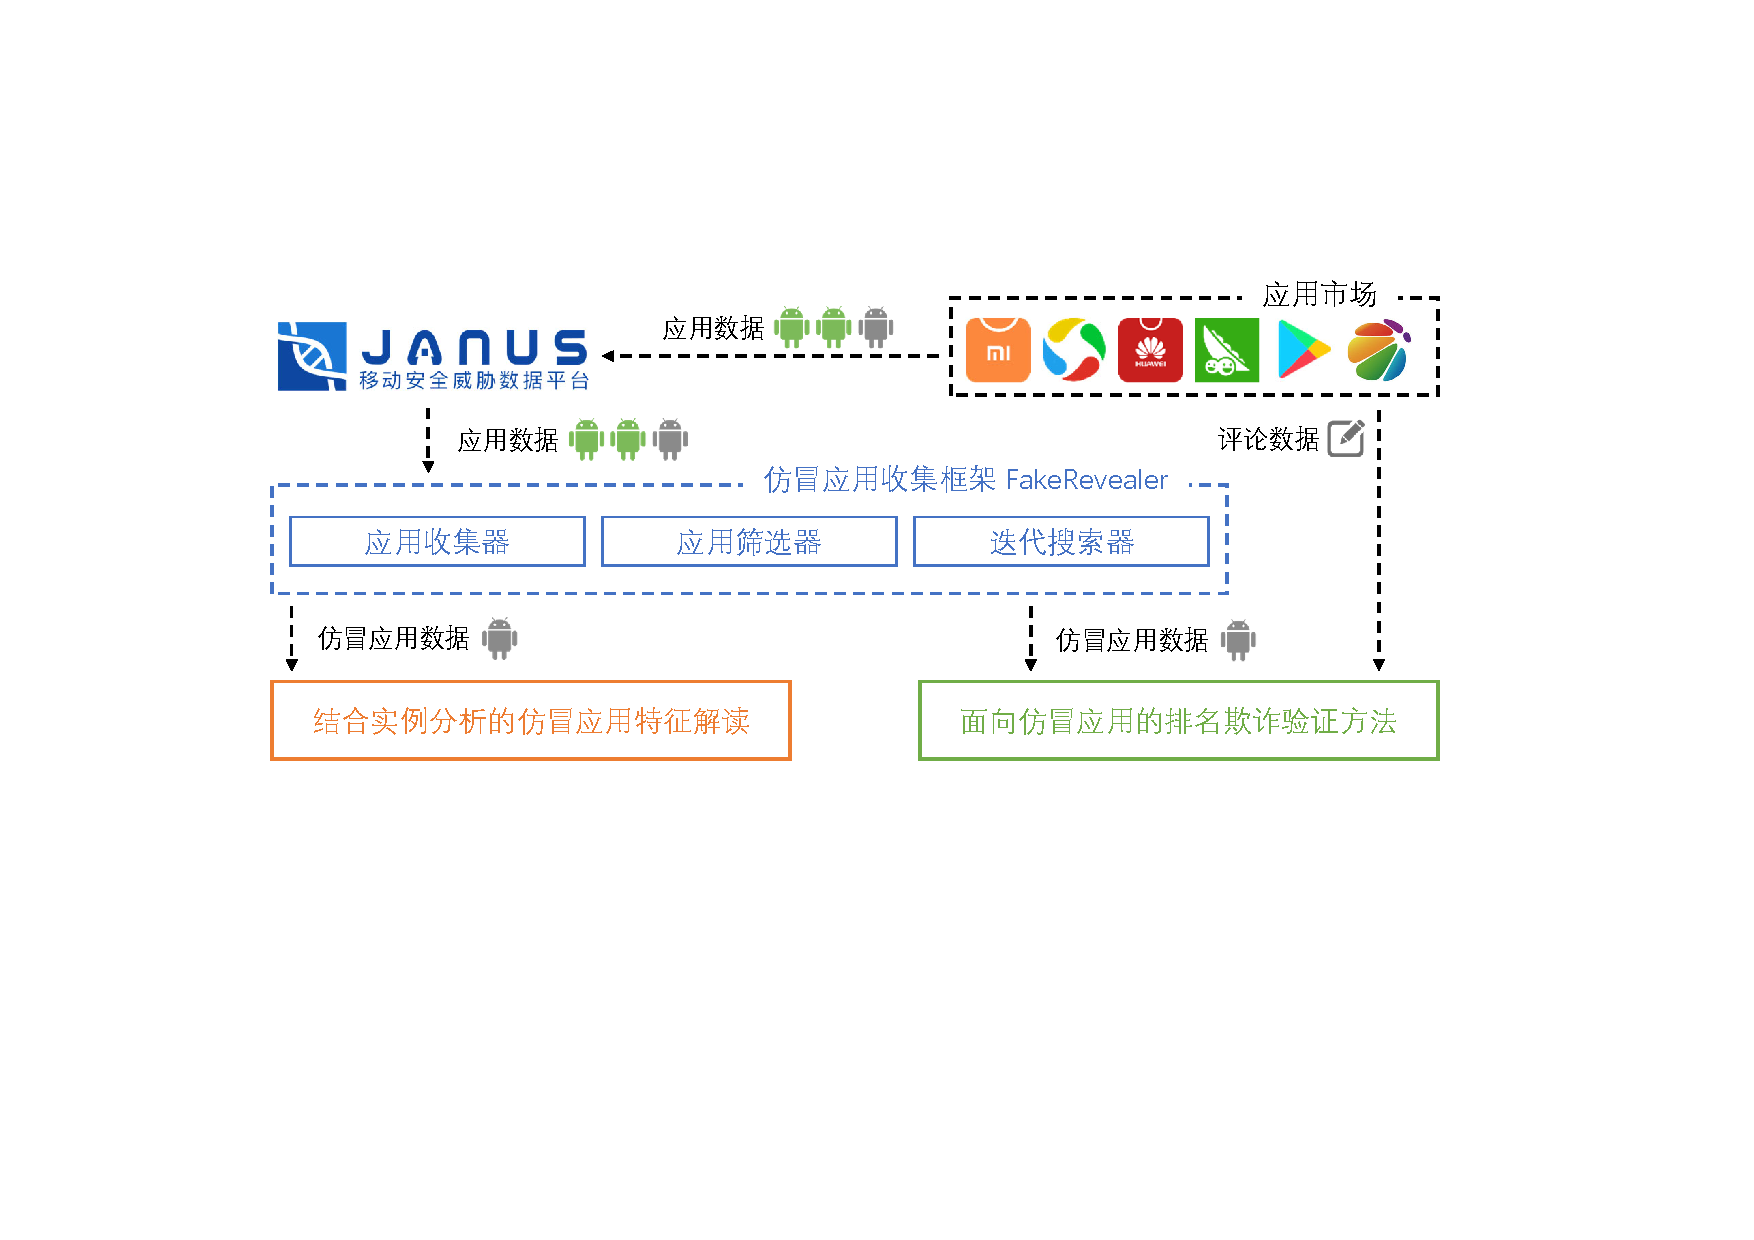
\includegraphics[width=\textwidth]{./Figures/edwin-overview}
% 	\caption{本文研究流程}
% 	\label{fig:Workflow}
% 	\vspace{-3mm}
% \end{figure}

% Fig.~\ref{fig:Workflow} shows the workflow of our study, which can be divided into two main phases:
% \autoref{fig:Workflow} 展示了本次实证研究的流程,其可以分为四个主要阶段:

% 1)\ \emph{数据收集} \quad
% 数据收集主要分为两个部分:正版应用信息的收集和仿冒应用的收集。
% 在正版应用信息收集的部分,本文选择了50个最热门的App作为目标应用,然后手动收集了跟这些App有关的信息;
% 仿冒应用信息收集方面,作者得到了上海犇众信息技术有限公司的帮助,得以接触从各个应用商店获得的大量的应用样本。
% 借助自动化分析框架\mytool,作者获得了大量仿冒应用的数据。

% 2)\ \emph{大规模数据挖掘} \quad
% 在这一步,我们对搜集到的仿冒样本数据进行分析,从三个视角完成了一次大规模数据挖掘。
% 三个视角分别是仿冒的基本应用特征、影响仿冒应用数量的因素和仿冒应用的发展轨迹,由浅入深,帮助读者理解仿冒应用的生态。

% 3)\ \emph{仿冒案例分析} \quad
% 之后,我们从收集的数据中选择了3个案例进行更深入的分析。
% 这三个案例在支持数据挖掘中的发现之外,揭示了更多仿冒应用开发者的行为特征。

% 4)\ \emph{市场反馈分析} \quad
% 在这个部分,我们从第三方应用市场中随机选取一部分应用,提取了用户对它们的所有历史评价,然后筛选出其中对仿冒应用的评价并分析,以期了解用户对这些应用持有的态度。
% 此基础上,我们还检测了仿冒应用与排名欺诈行为的关系,揭示移动黑灰产不同环节之间的关联。

\section{研究对象}
仿冒应用是一个跟正版应用相对的概念,所以需要先定义正版应用,再对仿冒应用进行探究。
因此,本研究先选取了一部分正版应用作为目标应用,再根据正版应用的信息搜寻仿冒应用,对搜集到的样本进行研究。

文献~\cite{kitchenham2002preliminary}指出,实证研究需要确保数据的准确性与全面性。
若在市场直接中随机挑选应用,将难以解释搜集到的应用是正版或是仿冒应用,进而不能保证数据的准确性,随机选取法并不适用于正版应用的选取。
因此,本研究参考了数据平台易观千帆的月度App排行榜~\cite{yiguanqianfan}。
该排行榜对超过1200个主流应用中的用户分享数据进行分析,汇总成应用热度(月度活跃用户数),按热度对应用进行排行。
一方面,该排行榜的数据来源是各应用``应用体验计划''中搜集所得的数据,数据本身具有一定真实性,可满足文献的准确性要求;
另一方面,排行榜中的应用均为主流应用,由知名度较高的开发者(如腾讯、百度、阿里巴巴等)开发,可认为排行榜上的应用均为正版应用,免去需要对搜集到的目标应用进行甄别的步骤;
此外,排行榜中的应用涵盖了多个领域,包括社交网络、资讯、移动购物、视频等,能满足数据收集中的全面性要求。
综上,从易观千帆平台选择目标应用是较为合适的方式。

\begin{table}[htbp]
	\renewcommand{\arraystretch}{1}
	\small
	\centering
	\caption{目标应用类别与各分类下应用}
	\vspace{1mm}
	\begin{tabular}{l c}
		\toprule
		{\bf 应用类别}                            & {\bf 应用名}                                               \\
		\midrule
		{社交网络}                                & {微信、QQ、新浪微博}                                       \\
		\rowcolor{gray!15}视频                    & {爱奇艺、腾讯视频、优酷、快手、抖音、火山小视频、西瓜视频} \\
		{生活}                                    & {支付宝、高德地图、百度地图、美团、墨迹天气、滴滴出行}     \\
		\rowcolor{gray!15}移动购物                & {淘宝、京东、拼多多}                                       \\
		\multirow{2}*{系统工具}                   & {WiFi万能钥匙、搜狗输入法、腾讯手机管家、360手机卫士、}    \\
		~                                         & {猎豹清理大师、360清理大师、WiFi管家、讯飞输入法}          \\
		\rowcolor{gray!15}                        & {百度、腾讯新闻、QQ浏览器、今日头条、}                     \\
		\rowcolor{gray!15} \multirow{-2}{*}{资讯} & {UC浏览器、网易新闻}                                       \\
		\multirow{2}*{应用市场}                   & {应用宝、华为应用市场、OPPO应用市场、}                     \\
		~                                         & {360手机助手、百度手机助手、小米应用市场}                  \\
		\rowcolor{gray!15}{音乐}                  & {酷狗音乐、QQ音乐、酷我音乐盒、全民K歌、网易云音乐}        \\
		{游戏}                                    & {王者荣耀、开心消消乐}                                     \\
		\rowcolor{gray!15}{摄影录像}              & {美图秀秀、美颜相机}                                       \\
		{商务办公}                                & {WPS Office、QQ邮箱}                                       \\
		\bottomrule
	\end{tabular}
	\label{table:taget_app}
\end{table}

该平台月度App排行榜的排名前50的热门应用被挑选作为本文的目标应用。
从功能角度入手,50个App被归入11个类别,分别为社交网络、视频、生活、移动购物等,详情可见\autoref{table:taget_app}。
作者手动从这50款App的官方网站上下载了这批应用的最新版本,作为正版应用的参考版本,寻找与之相关的仿冒应用进行后续研究。


\section{数据收集}
鉴于目前学术界中与仿冒应用直接相关的数据集较为稀缺,从工业界中系统地收集所需的仿冒应用数据来完成本次调研是最为直观合适的方法。
本节先根据上述的研究问题划定本研究所需的研究数据类型,再介绍如何对数据进行收集。

% \noindent {\bf Collected Dataset.}
\subsection{数据类型与收集方式}

综合研究问题,本研究需获取的数据类型可分为以下两部分:一、分析仿冒应用特征所需的应用基本信息;二、分析应用发布特征所需的应用证书信息、上架时间等元数据。

确定目标应用后,可在市场中寻找与目标应用相似的应用,提取其数据整理成集,满足一、二部分的数据需求。
但要获取足量的仿冒应用数据以组成数据集是一个较有挑战性的任务,有难点如下:
\begin{itemize}
	\item 研究者要从多个不同的应用市场中爬取App样本,每个应用市场都有不同的网页编码,甚至有反爬虫策略,不存在一个爬虫脚本对所有应用市场数据都通用的场景;
	\item 各个应用市场架上的App数量庞大,研究者需要有效地筛选出与目标应用有关的样本;
	\item 对于收集到的大量数据,研究者需要一个轻量级的解决方案快速判断获得的App样本为正版应用或是仿冒应用。
\end{itemize}

为应对第一个挑战,作者与工业界合作,利用犇众信息公司的Janus平台对各大应用商店进行样本爬取,获取应用样本信息。\footnote{此处平台与\secref{sec:signature}中提及的Android漏洞同名,但两者无直接关联,请注意区分。后文的``Janus平台''均指本平台,而``Janus漏洞''则特指Android漏洞。}
该平台自2017年起就开始对各大应用商店的App进行样本收集,可向用户提供各项App信息。
如\autoref{fig:Janus-data}显示,Janus平台至今已收集到上千万个App样本,可满足本研究数据采集需求。
除样本信息外,Janus平台也提供按规则搜索功能,用户可创建规则过滤平台中的应用数据,以获取所需应用App样本。
因此,视Janus平台为从各大应用市场中收集应用样本的代理,借助Janus平台获取各市场中的应用信息。

\begin{figure}[htbp]
	\centering
	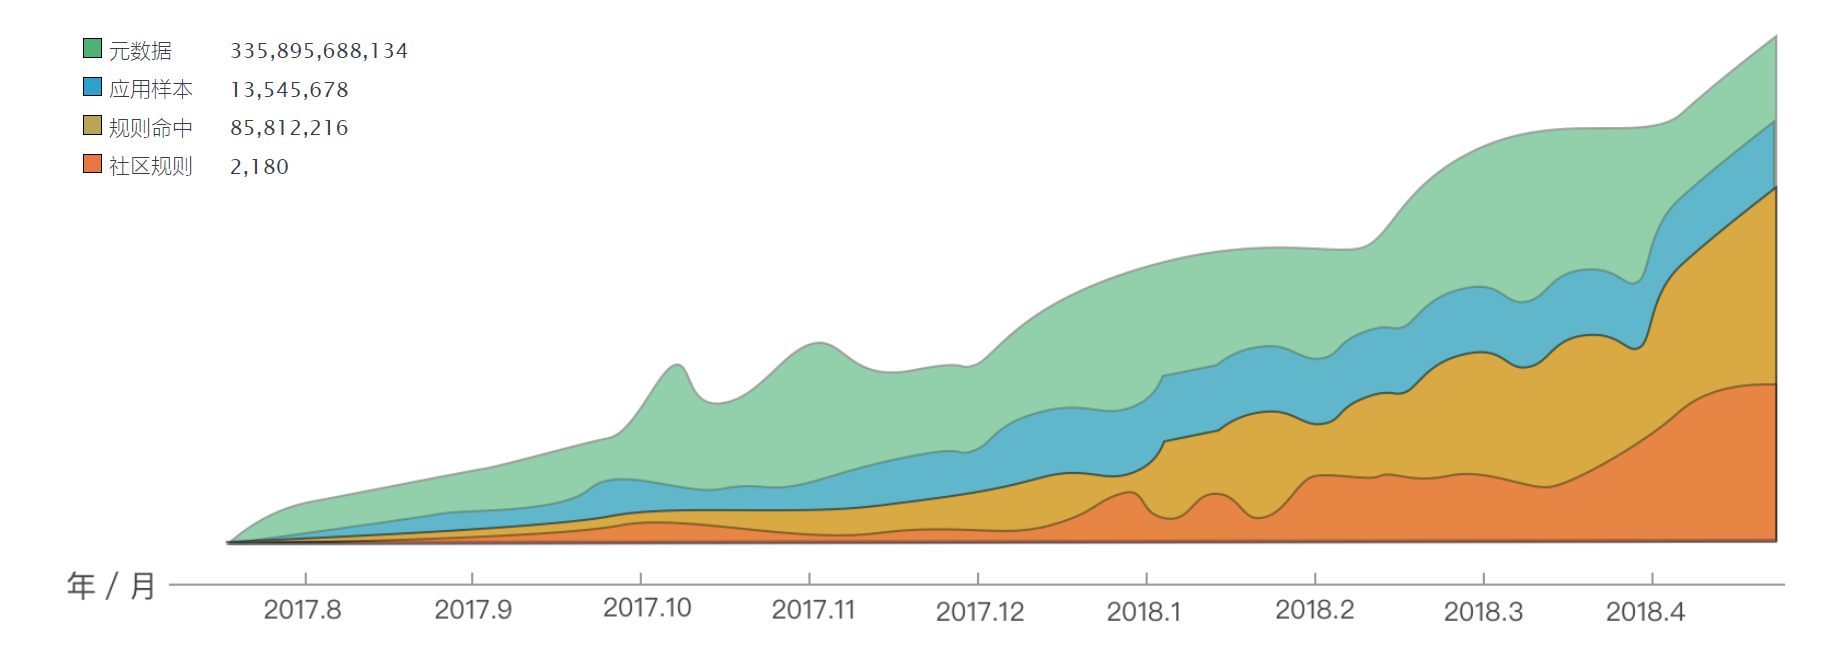
\includegraphics[width=\textwidth]{./Figures/edwin-Janus-data.png}
	\caption{Janus平台上的数据规模时序图}
	\label{fig:Janus-data}
	\vspace{-5mm}
\end{figure}


为应对第二个挑战,本研究提出了基于广度优先搜索(Breadth-First Search,简称BFS)算法的搜索框架(见\autoref{fig:FakeRevealer})。
具体地,对于每一款目标应用的收集流程分为三个部分:先以正版应用样本的\emph{包名}和\emph{应用名}作为查询条件放入迭代搜索器,迭代搜索器发出查询请求,从Janus平台中收集与目标应用相关的所有App样本,提取出样本的相关数据返回至应用收集器;
其后,应用收集器将数据转移至应用过滤器,利用过滤器判断收集到的应用数据源于正版应用或仿冒应用,保存仿冒应用数据,提取出正版应用的\emph{包名}和\emph{应用名};
最后,将上一步中获得的新的正版应用信息(\emph{包名}和\emph{应用名})再次放入迭代搜索器,开始下一次循环,从Janus平台中进行查询,获取更多与正版应用相关的样本。

\begin{figure}[htbp]
	\centering
	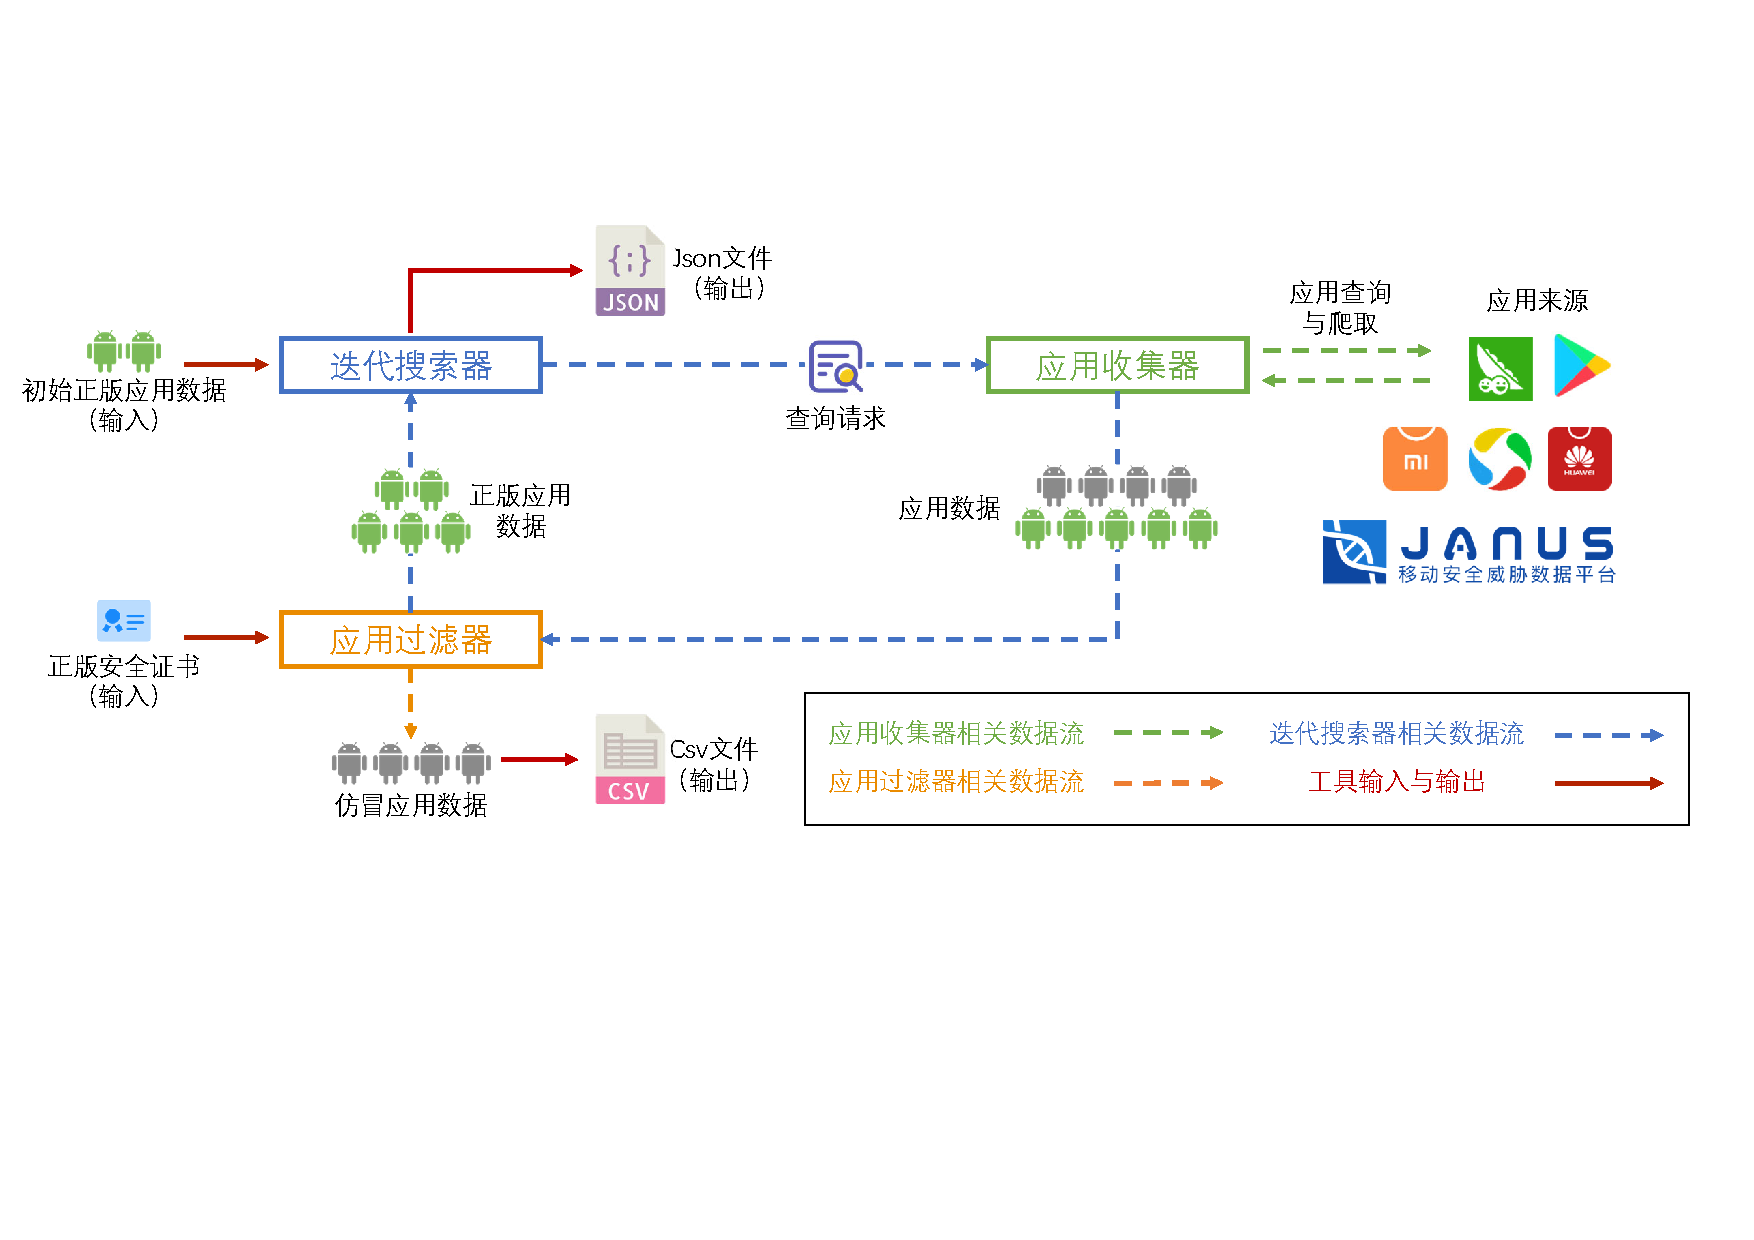
\includegraphics[width=\textwidth]{./Figures/edwin-fakerevealer}
	\caption{搜索框架整体流程}
	\label{fig:FakeRevealer}
	\vspace{-3mm}
\end{figure}

第三个挑战,可利用Android签名证书机制(详见第二章)解决。
对某个APK安装包而言,该机制提供了其被最后一次修改时的修改人信息。
因此,对于任一个被搜索框架收集到的APK,均可归入以下四种情况:

第一,该APK为正版应用,由正版开发者开发,也并未被篡改,应用证书与正版应用证书一致,是目标应用的某一版本(正版);
第二,该APK原本为正版应用,由正版开发者开发,使用旧版签名机制签署。由于APK采用了旧版签名,仿冒应用开发者利用漏洞篡改了部分数据,使样本成为仿冒应用,但应用证书并未被替换(仿冒);
第三,该APK原本为正版应用,被仿冒应用开发者解包篡改成为仿冒应用,但篡改是在解包后进行的,仿冒应用开发者无法通过原版证书为该APK重新打包,因此该APK的应用证书被替换为仿冒应用开发者的证书(仿冒);
第四,该APK由仿冒应用开发者开发,由于仿冒应用开发者不具有正版开发者的私钥,不能为该APK签署正版应用证书,因此该APK具有仿冒应用开发者的证书(仿冒)。

旧版签名机制存在漏洞,无法直接判断使用旧版签名机制签署、同时具备正版证书信息的APK文件是否曾被篡改。
然而,只要其应用证书信息与正版应用信息不符,无论其为被解包篡改的原正版应用,或是仿冒应用开发者重新开发的仿冒应用,均可划入仿冒应用范畴。
因此,本文在收集数据时,针对上述情况的第三、四种APK进行收集。

% 本研究从360手机助手应用市场中随机挑选了856个应用,爬取这批应用的所有评论作为第三部分数据。
% 国内应用商店市场监测报告~\cite{ChineseAppStoreReport}显示,360手机助手应用市场为国内占有市场份额最大的应用市场,以360手机助手为收集对象,可使数据具有一定代表性。
% 另外,与小米应用市场、OPPO应用市场等手机厂商推出的应用市场不同,360手机助手并非预置于手机系统中,因此可认为该应用市场用户喜好不与任一厂商的手机用户喜好强相关,在用户分布上具有更好的全面性。
% 对随机应用进行评论采集,而非针对特定应用进行评论采集也是出于相同考虑。
% 由于该856个应用为随机挑选所得,本研究认为这批数据具有一定的代表性,可反映整个市场的评论分布情况。

\subsection{数据概览}
\label{sec:data_overview}

% 如上节所述,本研究收集到的内容可分为两类:应用数据与评论数据。

% 应用数据方面,
从易观千帆提供的数据榜单中,本研究选择了分属11个不同的应用类别的50个最热门的App作为目标应用。
由于App的应用名可能会在App更新迭代的时候随之变更,作者用近似BFS的策略,从50种App中一共记录了198个不同的应用名以挖掘仿冒样本。

在这50款App中,以下三款App的样本并不能在市面上找到:\emph{OPPO 应用商店},\emph{华为应用商店}和\emph{小米应用商店}。
因为这三款App都是由手机设备厂商开发和预装在对应品牌的手机中的,仅供这些品牌的用户使用,并不在其他应用市场上提供下载。
当然,这也是这三款App热度高的原因——这几款App都被预装到了对应手机品牌厂商的每一部Android设备中,而OPPO、华为和小米又是国内最大的几家手机厂商,这几款App自然也会有庞大的用户基数。
因此,本研究最后的目标应用只有47款。

对这47款目标应用,搜索框架共检索到138,106个应用样本,样本源于29个不同渠道。
其中,69,614个应用样本持有官方开发者证书,52,638个应用样本并不具有官方证书。
余下部分应用样本为某些应用的发布在不同应用市场同一版本,在对各样本计算SHA1码去重筛选后被排除(共计15,854个)。
样本SHA1码是使用SHA1哈希算法对整个APK文件进行数据摘要之后获取到的编码串,可认为每个样本都有独一无二的SHA1码。

% 评论数据方面,本次研究一共爬取到了267,397名用户的365,461条评论,其中6款仿冒应用的所有历史评论共计3,591条,来自2,946名用户,每条评论数据由5项信息组成,除\emph{评论内容}、\emph{评价等级}和\emph{来源应用}三项必要信息外,还包括\emph{评论用户}与\emph{评论时间}以保留评论间的潜在联系。
% 在本研究收集评论的所有856个应用中,有6款应用与先前仿冒应用数据中的包名对应。
% 本研究的仿冒应用列表为针对50个热度最高的目标应用整理而成,而收集评论的应用在整个市场范围内随机挑选,此处仿冒应用占总体应用比例较小,不意味整个市场中的仿冒应用数量偏少。


\subsection{相关数据集对比}

作为软件工程方向的研究热点,Android应用研究一直广受关注。
在Android应用数据集方面,为推进Android恶意应用研究,一些安全厂商整理出了恶意应用数据集,使研究者免于数据收集之苦;部分论文中亦有公开的Android应用集可供参考。
较为著名的数据集有Android Malware Genome Project(Genome数据集),Drebin数据集,AMD数据集和AndroZoo数据集。

Genome数据集~\cite{Zhou2012DissectingAM}中的样本由Yajin Zhou等人持续收集一年余所得,其中包含了超过1,200个Android恶意应用,涵盖了收集时市面上存有的大部分恶意应用家族。
经过对数据集中恶意样本的详尽分析,Yajin Zhou等人总结了重打包、更新攻击和路过式下载(Drive-by Download)三种恶意应用的安装途径,并揭示了特权提升,远程控制,恶意扣费和信息收集四种恶意行为的方式,该数据集在后人研究中多被用于训练自动化恶意应用分类器。
该数据集收集的时间为2010年8月至2011年10月间,但已不再被维护。
Android系统在其后不断更新迭代,故其中的样本已有部分因兼容性问题不能再被安装到具有较新版本Android系统的设备上。
与该数据集类似的还有与2010年8月至2012年10月间收集的Drebin数据集~\cite{arp2014drebin},该数据集为Genome的超集,共包含涵盖了源于179个不同恶意应用家族的5,560个恶意样本。
AMD数据集~\cite{li2017android}则包含了从2010年至2016年间收集的24,553个样本,样本被分类至71个恶意应用家族的135个变种中,与Genome数据集和Drebin数据集相比,提供了更接近现状的恶意应用数据画像。
除去时间导致的兼容性问题,虽然Genome、Drebin和AMD三个数据集中的样本覆盖较为全面,但其收集对象已明确为产生恶意行为的``恶意应用'',而本文研究对象为模仿热门应用的仿冒应用,两者有所区别,因此直接使用三个数据集中的样本进行分析并不合适。

AndroZoo是一个仍在不断收集应用的数据集~\cite{li2017androzoo++}。
该数据集从包括Google Play应用商店、小米应用商店、安智网等多个数据源进行数据收集,现已包含超过一千两百万个应用样本。
一方面,AndroZoo的数据比前述数据集更新,更能反映应用市场现状;另一方面,比起Genome、Drebin和AMD三个针对恶意应用进行收集的数据集,AndroZoo收集的对象不限于恶意应用。
该应用集利用VirusTotal对所得的应用进行扫描,标记出被报告为恶意应用的样本;同时,维护者也整理了数据集中的重打包应用信息,为学者提供翔实的重打包应用相关的样本数据:该数据集的重打包应用目录共提供了2,776个原版应用样本对应的15,297个重打包样本。
与只针对恶意应用进行收集的数据集相比,同时收录重打包应用数据的AndroZoo数据集可用于更广泛的Android应用研究。
然而,重打包应用只是仿冒应用的其中一种形式,仿冒应用还包括仿照正版应用外观制作的应用程序,该数据集的重打包应用列表未能满足本文研究的数据需求。
因此,在对上述四个数据集进行调研对比后,作者选择重新构建仿冒应用数据集,以完成本文研究。

% 在评论数据集方面,已知数据集众多,大多源于大型网站。
% 大众点评于2011年11月至2013年11月期间收集了近万条评论~\cite{li2017bimodal};美国点评网站Yelp、TripAdvisor和电商网站Amazon各有其收集的真实数据,Yelp数据集包括了美国多家城市的数十万条餐厅点评~\cite{rayana2015collective, shehnepoor2017netspam},TripAdvisor数据集包括3万条评论~\cite{wu2010distortion},Amazon数据集中具有583万条评论,涵盖书籍、音乐、DVD/VHS等多个领域~\cite{jindal2008opinion};源于知名电影网站IMDB的评论数据集包含5万条影评~\cite{maas2011learning}。
% 少数数据集由学者在研究中公开,如Ott公布了其在相关研究中使用的数据集~\cite{ott2011finding},相关数据由两部分组成,真实数据部分从TripAdvisor中采集所得,虚假评论部分在Amazon的众包平台获取。
% 具体地,研究者在众包平台上以1美元为酬劳,请求用户对芝加哥的20家受欢迎酒店构想积极评论,以组成虚假评论数据集,最终得到了真实数据、虚假评论各400条的数据集。
% Li在后续研究~\cite{li2014towards}中扩充了该数据集,让其涵盖了酒店、餐厅和医院三个领域,并加入了来自领域专家的虚假评论。

% 已有评论数据集面向的领域众多,但本文前期调研显示,尚未有针对应用市场评论的数据集公开可用。
% 本研究收集应用市场的评论数据的目的是勘查仿冒应用是否具有排名欺诈行为,来自其他领域的评论数据集并不符合收集需求。
% 因此,本研究仍需自行采集数据。
% 以上评论数据集仍对本文评论数据收集有所启发:大型网站中可更易于获取有效数据,因此本研究的评论收集针对国内应用市场份额最大的360应用市场进行;
% 数据量应有一定规模,因此评论收集包括了近27万位用户的36万条评论;
% 同时,作者于调研时发现,Ott与Li的数据集仅包含评论文本与评论标签(即评论是否为虚假评论),并不有利于挖掘评论之间的潜在关联,所以作者特意从多维度收集评论数据,而非仅收集评论内容。


\section{本章小结}

本章主要对本研究进行了概览,提出了本文的主要研究问题,阐述了本研究的对象,并简述了数据的收集方式与收集结果。
最后,本章将数据集与其他已有数据集进行比较,解释为何重新收集数据,而非使用已有数据集。
% Empirical study is then applied to these metadata, especially to those of fake apps, to gain us a more comprehensive understanding on fake apps' nature and characteristics, and the behaviors of fake app authors.
% 下一章,我们将详述数据收集工具\mytool 的设计和实现。

\clearPaperPage

% \section{Large-scale Empirical Study and Discoveries}
\chapter{仿冒应用基本特征实证研究}
\label{chp:discoveries_basic}

上一章节介绍了本研究的相关设置,提出了7个与仿冒应用相关的研究问题。
本章从仿冒应用与原版应用相似度、影响应用被仿冒的严重程度的因素及仿冒应用行为三点入手,回答与仿冒应用基本特征相关的三个研究问题,即:

{\bf RQ1:仿冒应用和与之相对的正版应用的相似程度如何?}

{\bf RQ2:是否存在显著影响应用被仿冒的严重程度的单一因素?}

{\bf RQ3:仿冒应用作者制作出了怎样的仿冒应用?是否依然能提供原版应用的功能?}

\section{度量指标选择}
\label{sec:measure_selection}

为保证研究结构有效性,本节解析介绍本章研究用到的各度量指标以供参考。
为回答RQ1,本研究需要选择一种相似度指标衡量仿冒应用与原版应用的相似程度;
为回答RQ2,需要先选择一种指标衡量某款应用在受仿冒的严重程度程度,再将其与可代表应用热度、更新频率的指标相关联,以计算两者间的关联性。

\subsection{相似程度度量指标}

应用之间相似度可从多个层面定义,包括应用行为相似度,应用代码相似度以及应用外观相似度。
应用行为相似度量度需要案例与一定方式驱动样例(常用的为手动方式驱动,或利用UI Automator或Monkeys等工具预先录制好操作脚本再回放)。
考虑到采集到的的应用规模较大,且种类繁多,要对逐个应用设计、驱动样例的可行性并不高,因此本研究不对所有应用进行行为相似度比对。
应用代码相似度比对常用于重打包检测相关研究,核心为对两个应用间的代码进行比较,计算两者间重合范围。
然而,仿冒应用的意图为诱导用户下载安装,而代码层面的内容不在普通用户的可感知范围内。
因此,仿冒应用代码并不需要与原版应用相似,代码相似度不是在本研究场景下最为重要的相似度指标。
进一步推断可得,外观相似度是最符合本研究场景的相似度类别,仿冒应用开发者甚至可以重新开发与原版应用外观相似的应用骗取用户下载。
根据日常经验,用户对应用外观的可感知的因素有以下几点:应用图标、应用GUI界面、应用标题(包括包名与应用名)和应用大小。
基于采集到的数据,本研究利用应用标题与应用大小进行相似度比较。

在文本相似度比对方面,本研究采用\textit{编辑距离}~\cite{levenshtein1966binary}作为具体度量指标。
编辑距离是在自然语言处理(Natural Language Processing,简称NLP)领域被广泛应用的距离定义,其定义如下:

\begin{Def}
    编辑距离

    给定两个字符串$a$与$b$,其间的编辑距离$d(a, b)$为将$a$和$b$相互转换的最小编辑操作数。
    其中,每次添加、删除或将一个字符转换成另一个字符均算作一次编辑操作。
\end{Def}

例如,``jingdong''和``jindeng''之间的编辑距离是2,由前者转换为后者的其中一种编辑次数最小方法为将第一个``g''删除,再将``e''转成``o''。
同理,字符串``fake''和``official''之间的距离是7,其中一种方案为在``f''前添加``o'',在``f''和``a''之间添加``fici''(此处包含4步操作),将``k''替换作``l'',最后删去``e''。

\subsection{应用受仿冒严重程度相关度量指标}

本研究在衡量某款应用在仿冒应用开发者眼中受欢迎程度时,采用较为直观的指标:从直觉上看,市面上存在越多仿冒个体的应用,越受仿冒应用开发者欢迎(受仿冒程度越严重)。
但是,每款目标应用都有不同的样本数(官方样本数与仿冒样本数均有区别),不能直接以仿冒样本的数量作比较。
为消除偏差,本文将样本数量归一化,使用仿冒率对比每个目标应用在仿冒应用开发者中的受欢迎程度。

\begin{Def}
    仿冒率

    某款App~$a$的仿冒率$fake~sample~rate_a$指与其关联的仿冒样本的数量$fake_a$与该App正版样本的数量$total_a$的商;某应用市场$AS$的仿冒率$fake~sample~rate_{AS}$则是其中包含的所有目标应用的均值。
    两者可分别计算如下:
\end{Def}

\begin{equation}
    fake~sample~rate_a = \frac{fake_a}{total_a} \,,
    \label{equ:fake_rate_app}
\end{equation}
\begin{equation}
    fake~sample~rate_{AS} = Avg(fake~sample~rate_a, \forall a \in \text{\{目标应用\}}) \,.
    \label{equ:fake_rate_mkt}
\end{equation}

应用热度方面,研究直接取用从易观千帆平台取得的数据作为热度指标。
易观千帆平台为国内领先的应用数据收集平台,可认为其数据来源较为可靠。
更新频率指标方面,成熟的应用通常有较为固定的更新频率。
为评估目标应用的更新频率,本研究标记了每个官方应用样本被发行时的时间,精确到日,找到该应用的最新发布样本和最早发布样本,两者发行时间差值与中间版本数的商即为平均更新频率(单位:天/版本)。

\subsection{关联程度度量指标}

为探究应用受仿冒应用开发者的欢迎程度与其他因素的相关性,本研究利用皮尔逊积矩相关系数(Pearson product-moment correlation coefficient,简称PPMCC)计算一款App被仿冒的严重程度与其热度、更新频率是否具有相关性。

\begin{Def}
    皮尔逊积矩相关系数

    两个变量之间的皮尔逊相关系数定义为两个变量之间的协方差和标准差的商,计算公式如下:
\end{Def}
\begin{equation}
    p_{x,y} = corr(X,Y)=\frac{cov(X,Y)}{\sigma_x\sigma_y}=\frac{E[(X-u_x)(Y-u_y)]}{\sigma_x\sigma_y} \,.
    \label{equ:PPMCC}
\end{equation}
\autoref{equ:PPMCC}的值域为$[-1, 1]$。
该值越接近$1$,表示两个变量间存在正相关关系越强;越接近$-1$,表示两变量间存在的负相关关系越强;接近$0$,表示两个变量之间的相关关系弱。


\section{实证研究流程与结果解析}

本节分为四个部分,前三个部分分别针对章节起始的三个研究问题进行实证研究,最后一部分对实证研究结果进行有效性分析。

\subsection{仿冒样本与原版应用的相似度研究}

\noindent{\bf RQ1:仿冒应用和与之相对的正版应用的相似程度如何?}

先从统计数据入手探索数据:
包名方面,应用数据集统计结果显示,在所有的52,638个仿冒样本中,只有243个(少于0.5\%)使用了正版应用的包名,余下的所有仿冒样本都使用了自定义包名。
自定义包名的52,395个样本中,包含了14,089个不同的包名。
应用名方面则有截然不同的结果,大部分样本(41,863个,约79.5\%)使用了与原版应用一致的应用名,余下10,775个仿冒应用样本包含应用名共10,610个。
绝大部分仿冒应用并未保留原版应用的包名,但只有较少仿冒应用采用了新应用名。

作者推断,仿冒样本之所以极少直接沿用正版应用的包名,很可能与Android系统机制有关。
根据Android官方文档~\cite{setAppId}描述,每个Android应用都具备一个名为Application ID的属性,该属性为Android系统用于识别应用程序的唯一标识。
通常情况下,该属性与包名一致。
如果系统在安装App时发现系统中已经有具有相同Application ID的App,将检查两个应用的应用证书是否一致,证书不一致会导致安装失败。
因此大部分仿冒应用不会直接使用正版App的包名。
而应用名只有向用户展示的用途,不用于系统内的应用校验,系统也允许出现重复的应用名,所以大部分仿冒应用采用了与原版应用一致的签名以更好地诱导用户下载。

之后,研究采用如上节所述的外观相似度衡量指标,比对原版应用与仿冒应用之间的相似程度。
对于从仿冒样本中获取到的每个应用名,均计算与其对应的官方发布App的原版应用名的编辑距离;
同理,也计算出每个仿冒样本包名与原版包名的编辑距离,结果可见下图~\autoref{fig:Statistic_fake_and_official}。

\begin{figure*}[htbp]
    \centering
    \subfloat[应用名\label{fig:appname}]{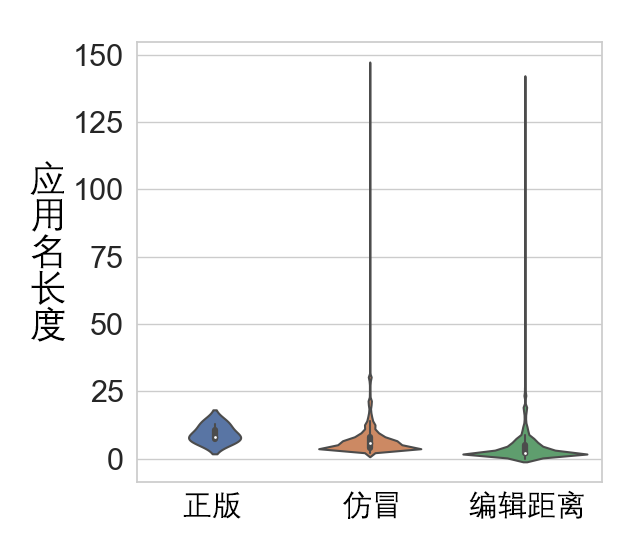
\includegraphics[width=0.333\textwidth]{./Figures/edwin-RQ1-2(a).png}}\hfill
    \subfloat[包名\label{fig:pkgname}]{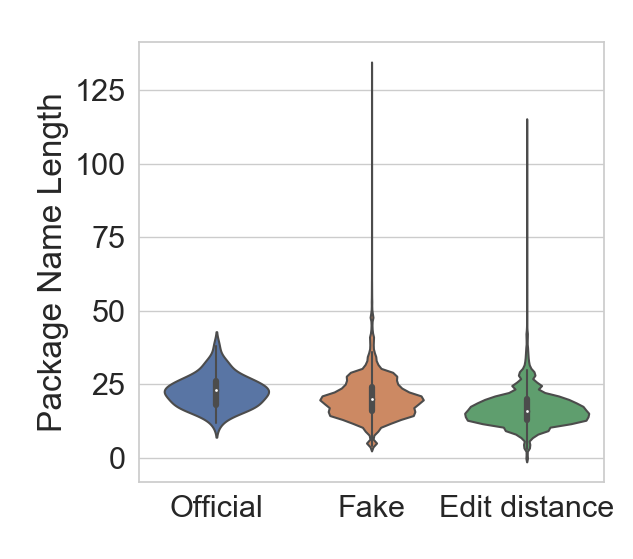
\includegraphics[width=0.333\textwidth]{./Figures/edwin-RQ1-2(b).png}}\hfill
    \subfloat[样本大小\label{fig:size}]{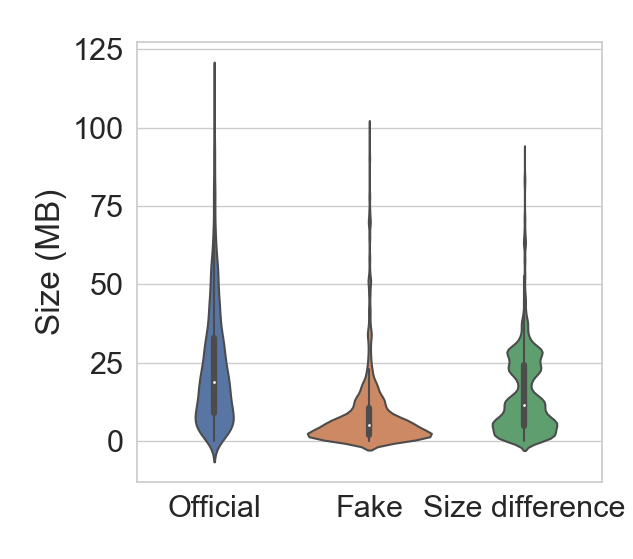
\includegraphics[width=0.333\textwidth]{./Figures/edwin-RQ1-2(c).png}}\hfill
    \caption{应用的应用名、包名与应用大小的相似性比较}
    \label{fig:Statistic_fake_and_official}
    \vspace{-5mm}
\end{figure*}

\autoref{fig:Statistic_fake_and_official}由三个小提琴图~\cite{violinplot}组成,分别表示了本文在应用名、包名和APK包大小上的统计信息。
每个``小提琴''的外部形状为数据的密度分布情况,小提琴中间的黑色粗条表示四分位数范围,粗条中小白点表示数据的中位数,黑色细条表示95\%置信空间范围。

\autoref{fig:appname}从左到右的三个图例分别展示官方样本、仿冒样本的应用名和两者间编辑距离的统计数据。
其中``正版''图例和``仿冒''图例中的中位数标志都接近数值``6'',说明官方样本和仿冒样本的应用名的平均长度十分相近。
``仿冒''图例整体分布具有集中性,较多样本分布在$y$轴数值为4到5之间,说明较多仿冒样本应用名长度落于此区间内。
``编辑距离''图例外部形状与``仿冒''图例大致类似,中位值十分低(在$y$轴上为``2''),意味着过半数仿冒应用通过从官方App的应用名中修改少于3个字符来获得其应用名。
上述结果表示大部分仿冒应用正在使用与官方App非常相似的应用名。
将三个图例与前文统计数据结合,可推断具备不同应用名的10,775个仿冒样本多数在原版应用名的基础上删减少量字符以获得新应用名。
同时,极少量仿冒应用有着异乎寻常的长名称(11个仿冒样本的应用名长度大于50个字符,最长的仿冒样本的应用名中甚至有146个字符)。
作者认为这部分异常样本可能是出于测试市场审查机制的目的被上传的。
此外,作者对部分具有长应用名的仿冒样本进行人工检查,一些长应用名拼合了多个热门App的名称(比如``潮流女装-美丽说蘑菇街淘宝天猫京东美团精选''或``老黄历万年历日历-农历天气预报知乎倒数日记账事本闹钟备忘录优步滴滴打车同花顺大智慧微博大众点评小说壁纸'')。
这可能是为了应用更容易地被用户搜索到而采取的策略。

\autoref{fig:pkgname}显示了针对包名的结果。
官方App的包名长度中位值和仿冒样本的包名长度中位值较为接近(双方的值分别为``23''和``20''),两者外形较为近似,说明原版样本与仿冒样本在包名长度上有类似分布。
然而,原版包名与仿冒样本包名之间编辑距离的中位数明显较高(在$y$轴上``16''的位置),这意味着将一个仿冒应用的包名转换为一个官方App的包名平均需要进行16次编辑。
换言之,官方App的包名和仿冒应用的包名有明显差异,仿冒应用更倾向于使用自定义且与原版应用有较大区别的包名。

\autoref{fig:size}则显示APK包大小的相关对比。
为了能更好地显示结果,部分极端样本在作图前被剔除出数据集:该部分样本为大于150MB的APK包,在所有69,614个官方App的样本中占851个(约为1\%),在52,638个仿冒样本中占447个(少于1\%),大部分来源于``游戏''类别下。
图表显示,仿冒样本大小的中位数约为5MB,约半数的正版App大小大于18MB。
``正版''图例中,应用大小样本分布相对均匀,密度曲线变化平缓,大部分样本分布于$(0, 60)$MB区间内,多数正版应用大小小于25MB,但在大于25MB的区间内仍有少量样本分布;
与之相比,``仿冒''图例的样本分布集中于3到4MB处,几乎没有样本大小大于25MB;
从该角度看,仿冒应用更有可能:

1) 由仿冒开发者自行开发,而非使用重打包技术制作。因为重打包之后的应用通常不会在大小上与原版有太大差距;

2) 是恶意应用。单独的恶意应用不需要包括较大的资源文件,只需少量具备恶意代码即可产生恶意行为;

\vspace{1mm}

简而言之,可从\autoref{fig:Statistic_fake_and_official}中获得两点总结,回答RQ1:

1) 更倾向于使用与正版App相似(甚至相同)的应用名,但包名与正版应用相差较大;

2) APK大小通常较小,很可能为仿冒应用开发者重新开发的恶意应用。
\vspace{1mm}


\begin{figure*}[t]
    \centering
    \subfloat[360应用市场\label{fig:360_detail}]{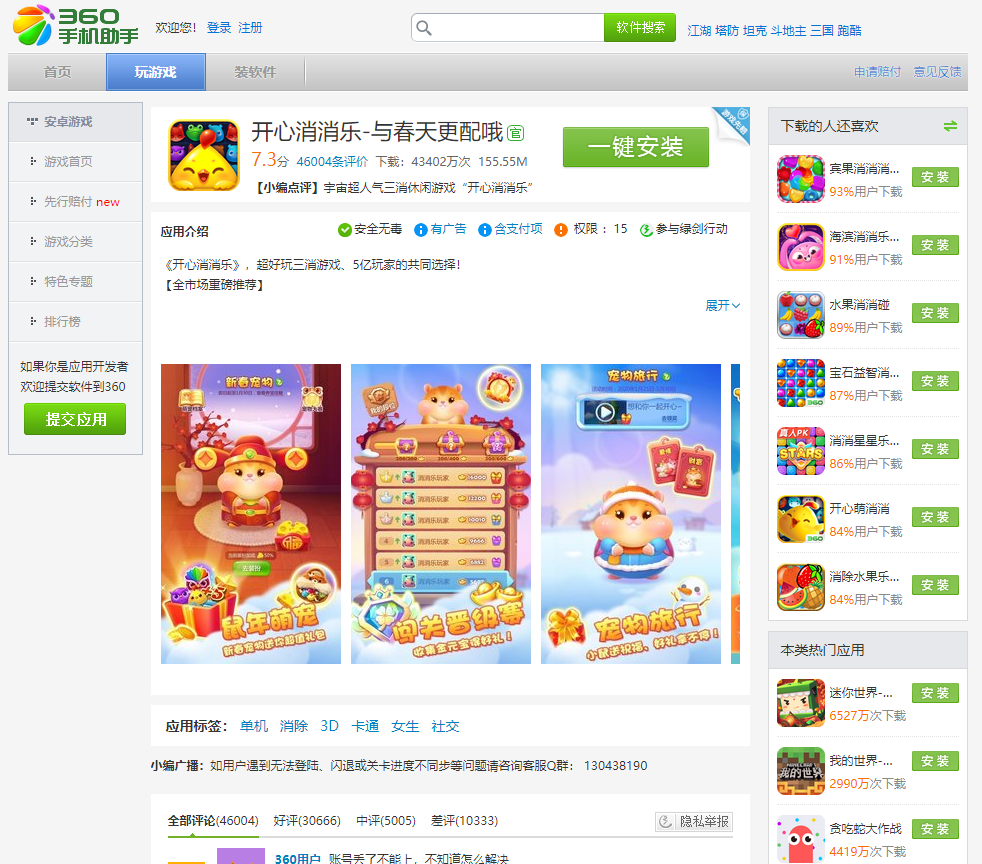
\includegraphics[width=0.49\textwidth]{./Figures/edwin-app-detail-360.png}}\hfill
    \subfloat[应用宝\label{fig:yyb_detail}]{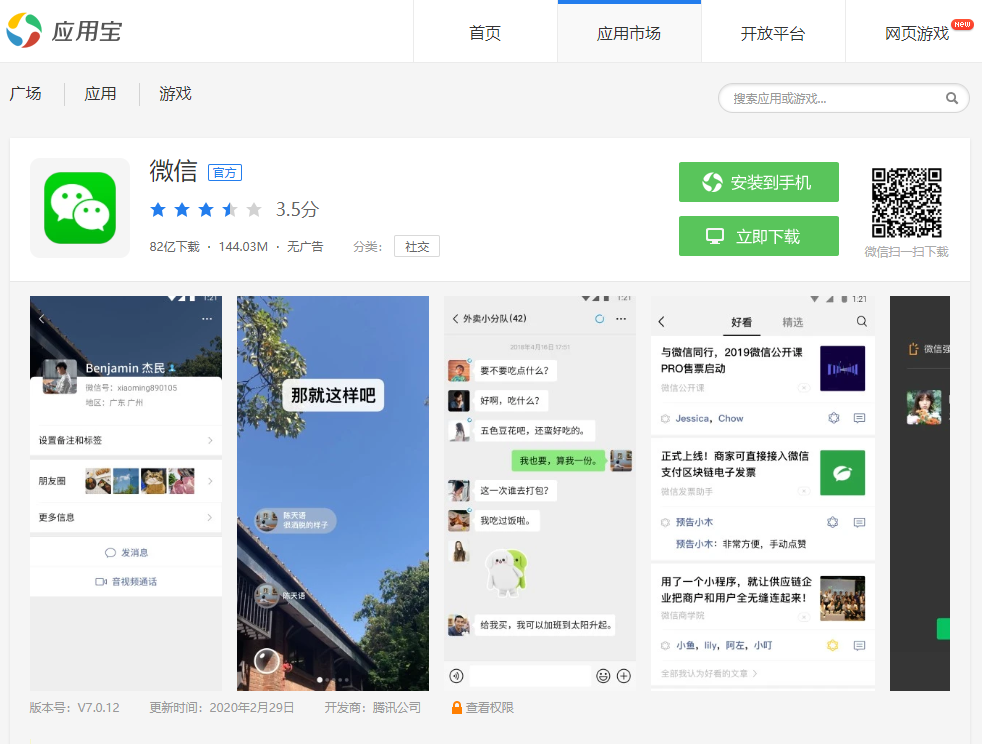
\includegraphics[width=0.49\textwidth]{./Figures/edwin-app-detail-yyb.png}}\hfill

    \subfloat[百度手机助手\label{fig:baidu_detail}]{
\includegraphics[width=0.49\textwidth]{./Figures/edwin-app-detail-baidu.png}}\hfill
    \subfloat[小米应用市场(部分信息被折叠)\label{fig:xiaomi_detail}]{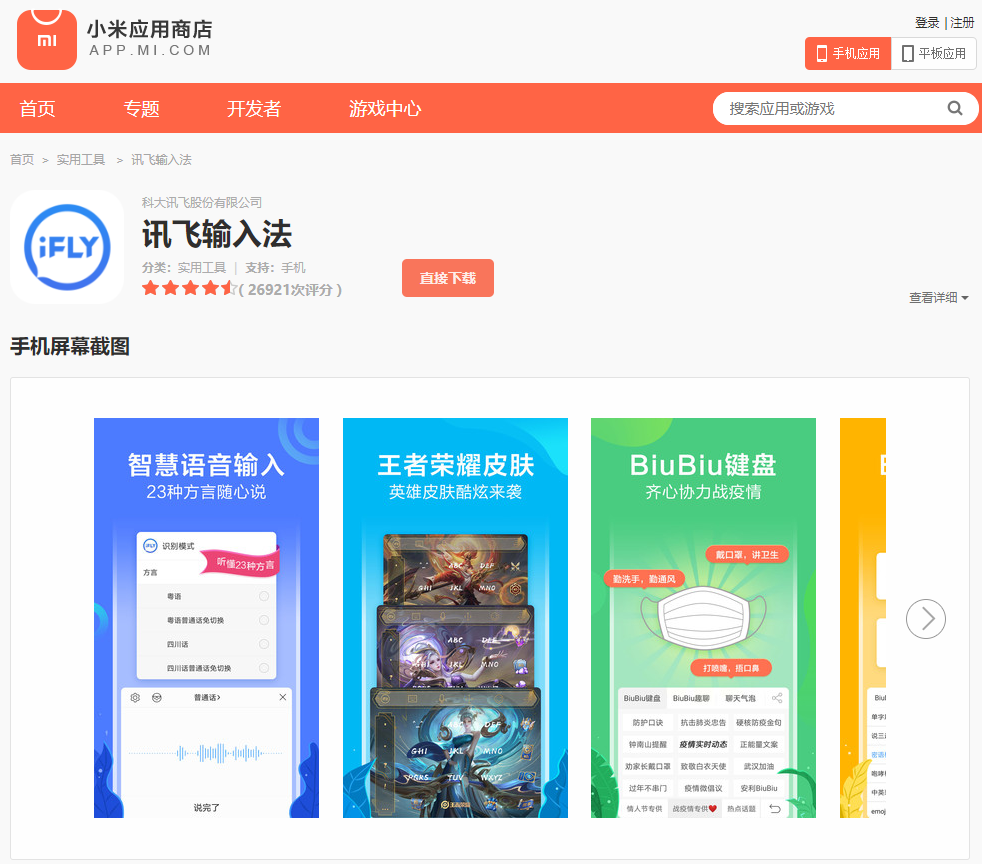
\includegraphics[width=0.49\textwidth]{./Figures/edwin-app-detail-xiaomi.png}}\hfill
    \caption{各大应用市场应用详情页}
    \label{fig:app_detail_page}
    \vspace{-5mm}
\end{figure*}

作者认为,造成上述第一点总结的原因是应用市场上提供的应用信息的不完备和用户对Android App了解的缺乏。
\autoref{fig:app_detail_page}显示了4个国内主流应用市场的详情页。
当用户浏览应用详情页时,各应用市场均显示对应应用的应用名、下载量、应用描述、其他用户对应用的评论和评分等信息。
但是,页面上较为醒目的条目是应用名、应用评分和图标信息,应用的技术参数(比如应用大小、版本号等)信息或是在不显眼处标记,或是被折叠,甚至不被展示。
在\autoref{fig:xiaomi_detail}所示的小米应用市场上,用户不能直接看到应用大小信息,需要点开折叠页才能获得相关数据。
上述四个应用市场应用详情页均不显示应用的包名信息。
由于普通用户不了解Android App中包名和应用名的区别和关联,展示相关信息对市场方引导用户下载安装应用也没有促进作用,市场对应用的技术参数展示并不重视。
因此,用户在应用市场上无法感知应用包名甚至应用大小,仿冒应用开发者无需在该两点上花费精力模仿正版应用。
相反,一方面,应用名在市场详情页上处于显眼位置,仿冒应用名称与正版越接近,越容易误导用户下载;另一方面,应用名重名不会在技术上造成阻碍。
因此,仿冒应用的应用名与正版应用十分类似,但包名、应用大小与正版应用相距较大。

\subsection{影响应用被仿冒的严重程度的因素研究}
\label{sec:quantitativeStudy}

\noindent{\bf RQ2:是否存在显著影响应用被仿冒的严重程度的单一因素?}

影响应用被仿冒的严重程度的因素众多,如能找到影响应用被仿冒的严重程度的主要因素,可针对性地制订策略防范仿冒应用。
根据经验,监管严格的应用市场上,仿冒应用更难通过审核;
一个应用的热度越高,越可能被仿冒应用开发者抄袭;
不同类别的应用具有不同目标人群,也可能影响仿冒应用开发者对其的态度。
因此,作者假设仿冒应用的数目与其来源市场相关,也受原版应用的热度、应用分类等因素影响。
App的更新频率也被视作影响仿冒数量的潜在因素,因为频繁更新的App或许可阻碍仿冒应用开发者对其进行仿冒。
根据上述因素,分别从应用所在市场与应用自身出发,作者将RQ2再细分为以下子问题:

{\bf RQ 2.1}:仿冒应用主要源于什么市场?仿冒率与市场规模是否有关系?

{\bf RQ 2.2}:某应用的热度/更新频率/所在类别是否影响其对应仿冒率?

\noindent{\bf RQ 2.1}:仿冒应用主要源于什么市场?仿冒率与市场规模是否有关系?

本研究中搜集的应用样本来源于多个不同的应用市场,不同市场规模不一,其审核、监管力度也并不一致。
根据各个样本的来源,有统计结果如\autoref{fig:Sample_source}。

\begin{figure*}[htbp]
    \centering
    \setlength{\belowcaptionskip}{-10pt}
    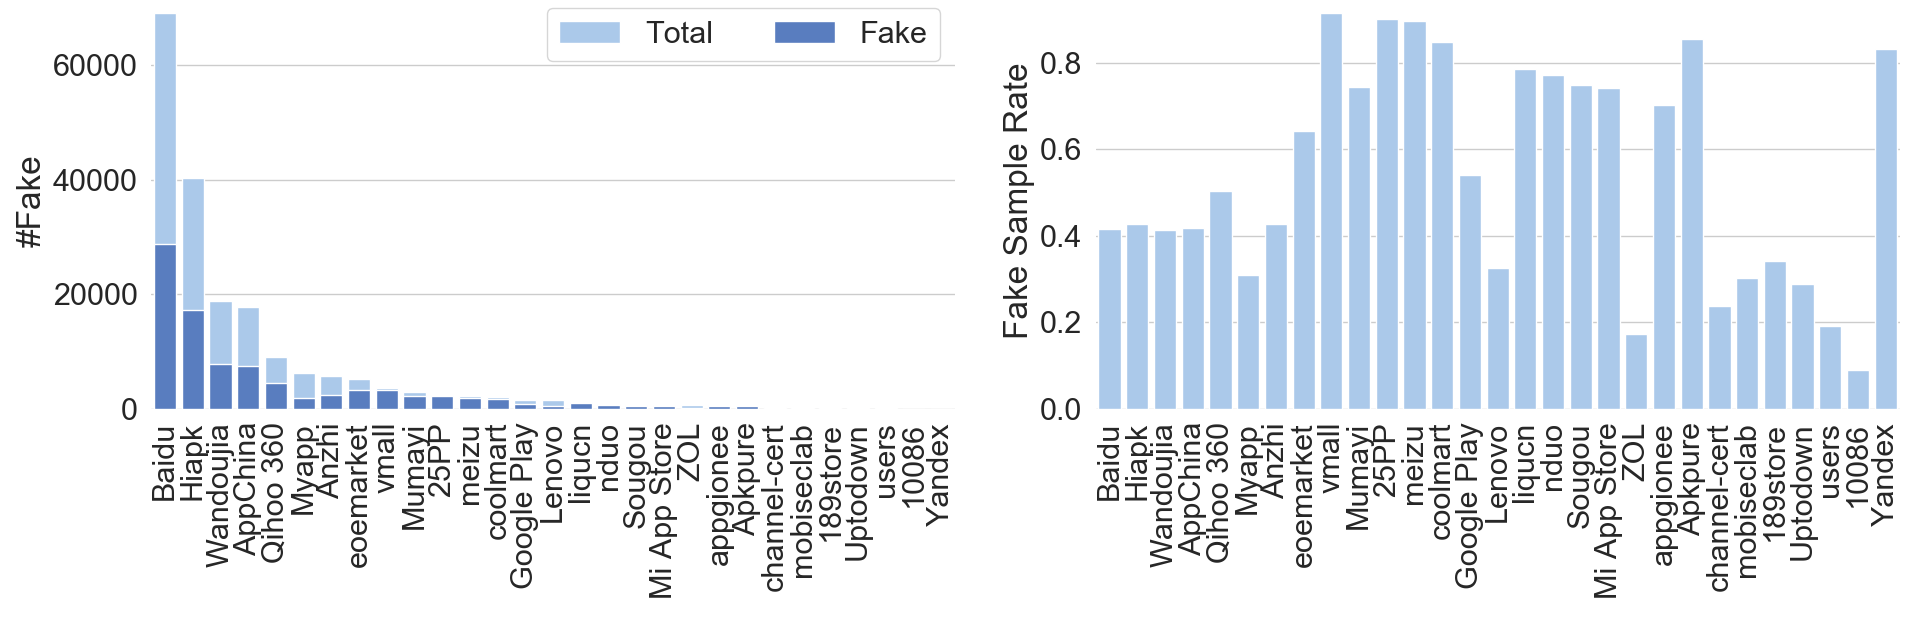
\includegraphics[width=\textwidth]{./Figures/edwin-Number_of_samples_collected_markets_3.png}
    \caption{从不同应用市场中收集到的应用数量以及各市场仿冒率}
    \label{fig:Sample_source}
\end{figure*}

左图显示,在本研究收集数据的所有29个应用来源中,从样本总数与仿冒样本数两个角度看,\texttt{百度手机助手}均提供了最多样本。
由于本研究选取的目标应用为市面上最受欢迎的应用,较有代表性,可将各渠道提供的样本量与国内市场规模相联系。
各个应用市场的仿冒率在右图呈现。


\texttt{百度手机助手}~\cite{Baiduappstore}和\texttt{安卓市场}~\cite{Hiapk}的仿冒率均约为40\%,在所有的29个渠道中处于中等水平,但由于源于该两个渠道样本基数最大,两者也提供了最多仿冒样本数。
由图中数据可得,应用市场的样本数量与仿冒率不直接相关。
然而,应用和市场的关系有可能对应用仿冒率产生影响:
本研究的50款目标应用中,有12款由腾讯公司开发,3款由360开发。
针对该15款应用进行仿冒率计算,得到各应用于规模较大的9个应用市场中仿冒率如下:

\begin{table}[htbp]
    \renewcommand{\arraystretch}{1}
    \footnotesize
    \centering
    \caption{15款应用于各大市场的仿冒率(数值单位:\%)}
    \vspace{1mm}
    \begin{tabular}{l c c c c c c c c c}
        \toprule
                                        & {\bf 百度} & {\bf 安卓市场} & {\bf 豌豆荚} & {\bf 应用汇} & {\bf 360} & {\bf 应用宝} & {\bf 安智} & {\bf 优亿} & {\bf 华为} \\
        \midrule
        QQ                              & 54.86      & 52.73          & 49.74        & 46.12        & 49.45     & 29.72        & 26.36      & 66.55      & 95.73      \\
        \rowcolor{gray!15} 微信         & 89.94      & 90.47          & 93.6         & 89.05        & 92.34     & 53.19        & 94.58      & 95.0       & 99.81      \\
        腾讯视频                        & 6.25       & 4.55           & 13.27        & 10.84        & 4.55      & 0.0          & 2.0        & 0.0        & 66.67      \\
        \rowcolor{gray!15} 腾讯手机管家 & 62.9       & 78.94          & 72.14        & 67.29        & 82.67     & 56.32        & 74.74      & 87.1       & 98.04      \\
        QQ音乐                          & 5.09       & 2.04           & 12.87        & 5.71         & 2.63      & 1.96         & 0.0        & 19.35      & 84.21      \\
        \rowcolor{gray!15} 开心消消乐   & 89.66      & 80.19          & 87.5         & 47.89        & 70.23     & 63.54        & 66.67      & 93.7       & 96.36      \\
        王者荣耀                        & 83.91      & 78.84          & 66.19        & 55.88        & 77.42     & 28.92        & 67.21      & 93.15      & 88.89      \\
        \rowcolor{gray!15} QQ邮箱       & 2.37       & 1.72           & 0.0          & 6.06         & 0.0       & 0.0          & 0.0        & 15.38      & 66.67      \\
        QQ浏览器                        & 2.18       & 2.47           & 10.78        & 1.98         & 6.52      & 0.0          & 2.7        & 15.79      & 90.0       \\
        \rowcolor{gray!15} 腾讯新闻     & 0.82       & 1.31           & 0.0          & 5.56         & 0.0       & 0.0          & 0.0        & 0.0        & 0.0        \\
        应用宝                          & 39.63      & 56.12          & 22.01        & 28.39        & 44.68     & 52.38        & 92.86      & 80.0       & 91.43      \\
        \rowcolor{gray!15} 全民K歌      & 42.86      & 43.01          & 35.78        & 55.77        & 60.38     & 23.81        & 49.06      & 35.29      & 66.67      \\
        360手机卫士                     & 65.92      & 46.2           & 79.56        & 74.78        & 67.27     & 91.46        & 82.05      & 83.08      & 96.1       \\
        \rowcolor{gray!15} 360清理大师  & 4.26       & 6.67           & 0.0          & 13.04        & 0.0       & 0.0          & 0.0        & 9.09       & 0.0        \\
        360手机助手                     & 33.89      & 68.0           & 17.89        & 45.21        & 19.48     & 30.0         & 37.5       & 15.79      & 87.5       \\
        \bottomrule
    \end{tabular}
    \label{table:firm_apps}
\end{table}

腾讯系的12款应用分别为QQ,微信,腾讯视频,腾讯手机管家,QQ音乐,开心消消乐,王者荣耀,QQ邮箱,QQ浏览器,腾讯新闻,应用宝和全民K歌;
360系的3款应用为360手机卫士,360清理大师和360手机助手。
应用宝为腾讯旗下应用市场,~\autoref{table:firm_apps}中结果表明,应用宝中腾讯系应用仿冒率明显比其他市场低;
同样地,360系应用在360市场中的仿冒率也比其他市场中明显降低。
作者猜测,应用宝对12款腾讯系应用相关的应用有较为严格的审核流程,有效遏制了该市场中与上述12款腾讯系应用相关的仿冒应用。
同理,360系应用在360市场中仿冒率较低。

结果表明,应用市场的规模与仿冒率无明显关联,但应用本身与市场的关系对仿冒率有影响。

\noindent{\bf RQ 2.2}:某应用的热度/更新频率/所在类别是否影响其对应仿冒率?

通常,某款App越受欢迎,其对应的仿冒应用越有可能被用户误下载,令仿冒应用开发者获取利润,吸引更多仿冒应用开发者对其仿冒;
应用更新可被分为功能性更新与安全性更新两类,频繁更新的应用功能迭代速度快,复杂度高,也可能有更好的安全性,使仿冒开发者难以复刻;
不同类别的应用具有不同目标人群与功能,也可能影响对应的应用被仿冒的严重程度。
针对上述前两个因素,本节使用皮尔逊积矩相关系数衡量仿冒率与因素对应维度指标的关联性;由于类别无法用连续变量表示,相关系数不适用于该因素,本研究将以图表形式表示两者之间的关联程度。

热度数据源于易观千帆平台;
应用更新频率取自某应用最早版本与最新版之间的平均更新时长,即两者发行时间差值与中间版本数的商;
根据应用功能划分,本研究的50款目标应用被分为11个类别,分别为应用市场,摄影录像,游戏,资讯,生活,音乐,移动购物,商务办公,社交网络,系统工具,视频。

\begin{ThreePartTable}
    \centering
    \renewcommand{\arraystretch}{1.05}
    \footnotesize
    \setlength{\belowcaptionskip}{-5pt}
    \vspace{1mm}
    \begin{longtable}{l l c c c c c c}
        \caption{目标应用与其相关统计}\label{table:data-statistics}                                                                                                                                      \\
        \toprule
        {\bf 应用名}                    & {\bf 类别} & \begin{tabular}[c]{@{}c@{}}{\bf 月度热} \\ {\bf 度指数} \end{tabular} & \begin{tabular}[c]{@{}c@{}}{\bf 更新频率} \\ {\bf (天/版本)} \end{tabular} & {\bf 样本总数} & \begin{tabular}[c]{@{}c@{}}{\bf 仿冒} \\ {\bf 样本数} \end{tabular} & {\bf 仿冒率} & \begin{tabular}[c]{@{}c@{}}{\bf 平均仿冒} \\ {\bf 延迟(天)} \end{tabular} \\
        \midrule
        微信                            & 社交网络   & 91.2K                      & 6.4                        & 9248           & 6447                       & 69.7\%       & 12.1                       \\
        \rowcolor{gray!15} QQ           & 社交网络   & 54.6K                      & 10.7                       & 11167          & 3780                       & 33.8\%       & 9.2                        \\
        爱奇艺                          & 视频       & 53.5K                      & 6.4                        & 7586           & 3481                       & 45.9\%       & 9.3                        \\
        \rowcolor{gray!15} 支付宝       & 生活       & 48.1K                      & 10.2                       & 983            & 231                        & 23.5\%       & 10.1                       \\
        淘宝                            & 移动购物   & 47.5K                      & 7.0                        & 6003           & 3010                       & 50.1\%       & 8.1                        \\
        \rowcolor{gray!15} 腾讯视频     & 视频       & 47.3K                      & 6.3                        & 1429           & 68                         & 4.8\%        & 10.7                       \\
        优酷                            & 视频       & 40.9K                      & 7.3                        & 2058           & 262                        & 12.7\%       & 6.7                        \\
        新浪微博                        & 社交网络   & 39.2K                      & 5.3                        & 5947           & 2715                       & 45.7\%       & 5.7                        \\
        \rowcolor{gray!15} WiFi万能钥匙 & 系统工具   & 36.4K                      & 3.1                        & 4808           & 2999                       & 62.4\%       & 3.0                        \\
        搜狗输入法                      & 系统工具   & 33.3K                      & 11.0                       & 898            & 40                         & 4.5\%        & 21.8                       \\
        \rowcolor{gray!15} 百度         & 资讯       & 32.4K                      & 11.1                       & 15651          & 3514                       & 22.5\%       & 12.8                       \\
        腾讯新闻                        & 资讯       & 28.7K                      & 8.5                        & 1051           & 11                         & 1.0\%        & 8.9                        \\
        \rowcolor{gray!15} QQ浏览器     & 资讯       & 27.8K                      & 5.6                        & 1369           & 43                         & 3.1\%        & 11.6                       \\
        今日头条                        & 资讯       & 27.4K                      & 4.4                        & 3538           & 179                        & 5.1\%        & 5.6                        \\
        \rowcolor{gray!15} 应用宝       & 应用市场   & 27K                        & 11.4                       & 2419           & 266                        & 11.0\%       & 11.6                       \\
        快手                            & 视频       & 24.4K                      & 3.2                        & 8273           & 4270                       & 51.6\%       & 3.5                        \\
        \rowcolor{gray!15} 腾讯手机管家 & 系统工具   & 24.2K                      & 8.7                        & 2463           & 1340                       & 54.4\%       & 8.7                        \\
        高德地图                        & 生活       & 24K                        & 6.5                        & 1225           & 51                         & 4.2\%        & 13.1                       \\
        \rowcolor{gray!15} 酷狗音乐     & 音乐       & 23K                        & 8.6                        & 1313           & 122                        & 9.3\%        & 12.2                       \\
        QQ音乐                          & 音乐       & 21.7K                      & 9.4                        & 1132           & 65                         & 5.7\%        & 14.6                       \\
        \rowcolor{gray!15} 百度地图     & 生活       & 21.3K                      & 8.8                        & 2609           & 1438                       & 55.1\%       & 15.3                       \\
        抖音                            & 视频       & 19.4K                      & 11.1                       & 317            & 12                         & 3.8\%        & 8.3                        \\
        \rowcolor{gray!15} 京东         & 移动购物   & 18.5K                      & 10.9                       & 5000           & 2377                       & 47.5\%       & 12.3                       \\
        UC浏览器                        & 资讯       & 16.7K                      & 7.4                        & 4232           & 1624                       & 38.4\%       & 7.0                        \\
        \rowcolor{gray!15} 360手机卫士  & 系统工具   & 15.4K                      & 12.4                       & 3670           & 1423                       & 38.8\%       & 19.1                       \\
        全民K歌                         & 音乐       & 14.7K                      & 21.1                       & 618            & 215                        & 34.8\%       & 17.3                       \\
        \rowcolor{gray!15} 美团         & 生活       & 13K                        & 8.0                        & 4752           & 1415                       & 29.8\%       & 6.9                        \\
        拼多多                          & 移动购物   & 12.9K                      & 6.6                        & 2327           & 551                        & 23.7\%       & 7.8                        \\
        \rowcolor{gray!15} 王者荣耀     & 游戏       & 12.5K                      & 15.5                       & 2350           & 1319                       & 56.1\%       & 12.3                       \\
        美图秀秀                        & 摄影录像   & 12.4K                      & 5.4                        & 1705           & 784                        & 46.0\%       & 5.8                        \\
        \rowcolor{gray!15} 火山小视频   & 视频       & 12.2K                      & 11.9                       & 410            & 16                         & 3.9\%        & 9.6                        \\
        墨迹天气                        & 生活       & 12K                        & 4.2                        & 10081          & 7093                       & 70.4\%       & 4.7                        \\
        \rowcolor{gray!15} 滴滴出行     & 生活       & 11.8K                      & 8.6                        & 943            & 117                        & 12.4\%       & 7.0                        \\
        华为应用市场                    & 应用市场   & 11.8K                      & N/A                        & 0              & 0                          & 0.0\%        & N/A                        \\
        \rowcolor{gray!15} 开心消消乐   & 游戏       & 11.2K                      & 19.7                       & 2406           & 1738                       & 72.2\%       & 20.6                       \\
        酷我音乐盒                      & 音乐       & 11K                        & 2.9                        & 3778           & 69                         & 1.8\%        & 4.2                        \\
        \rowcolor{gray!15} 西瓜视频     & 视频       & 11K                        & 11.5                       & 866            & 100                        & 11.5\%       & 8.8                        \\
        OPPO应用商店                    & 应用市场   & 10.8K                      & N/A                        & 0              & 0                          & 0.0\%        & N/A                        \\
        \rowcolor{gray!15} 猎豹清理大师 & 系统工具   & 9.9K                       & 10.3                       & 1803           & 388                        & 21.5\%       & 13.5                       \\
        360清理大师                     & 系统工具   & 9.6K                       & 17.3                       & 327            & 8                          & 2.4\%        & 8.5                        \\
        \rowcolor{gray!15} 360手机助手  & 应用市场   & 9.2K                       & 7.6                        & 1616           & 137                        & 8.5\%        & 8.4                        \\
        WiFi管家                        & 系统工具   & 8.8K                       & 19.5                       & 1636           & 658                        & 40.2\%       & 15.7                       \\
        \rowcolor{gray!15} 讯飞输入法   & 系统工具   & 8.6K                       & 6.0                        & 1451           & 8                          & 0.6\%        & 10.1                       \\
        百度手机助手                    & 应用市场   & 8.2K                       & 11.4                       & 3849           & 437                        & 11.4\%       & 14.5                       \\
        \rowcolor{gray!15} 小米应用市场 & 应用市场   & 7.8K                       & N/A                        & 0              & 0                          & 0.0\%        & N/A                        \\
        WPS Office                      & 商务办公   & 7.4K                       & 6.0                        & 1152           & 69                         & 6.0\%        & 7.8                        \\
        \rowcolor{gray!15} 美颜相机     & 摄影录像   & 7.1K                       & 5.3                        & 1600           & 691                        & 43.2\%       & 6.3                        \\
        网易云音乐                      & 音乐       & 7K                         & 10.5                       & 616            & 6                          & 1.0\%        & 12.2                       \\
        \rowcolor{gray!15} 网易新闻     & 资讯       & 6.7K                       & 7.0                        & 1441           & 93                         & 6.5\%        & 5.0                        \\
        QQ邮箱                          & 商务办公   & 6.6K                       & 16.4                       & 520            & 11                         & 2.1\%        & 10.4                       \\
        \bottomrule
    \end{longtable}
    \vspace{-4mm}
\end{ThreePartTable}

\begin{figure*}[htbp]
    \centering
    \setlength{\belowcaptionskip}{-10pt}
    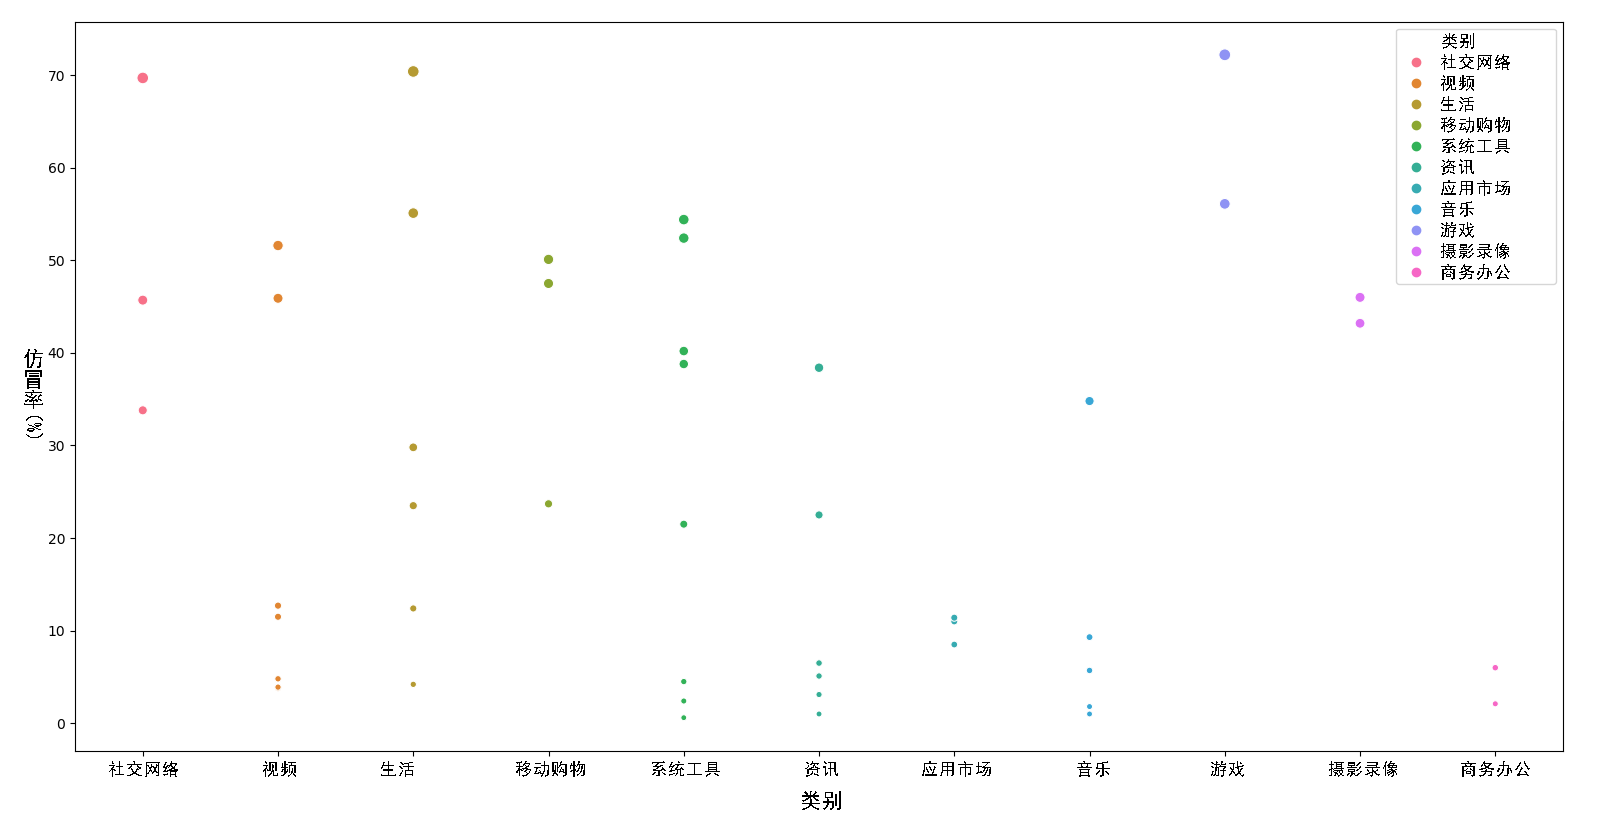
\includegraphics[width=\textwidth]{./Figures/edwin-category-fake-rate.png}
    \caption{目标应用类别-仿冒率对应图}
    \label{fig:category_fake_rate}
\end{figure*}

\autoref{table:data-statistics}按每款App的热度排序,展示了每款目标应用的类别、仿冒率、更新频率、关联样本总数等数据。
将数据代入\autoref{equ:PPMCC}可分别获得应用热度、更新频率与仿冒率之间的关联程度。
~\autoref{fig:category_fake_rate}显示每款目标应用所在类别及其仿冒率的对应关系,如$x$轴社交网络上对应的三个粉色圆点为三个社交网络类别下目标应用的仿冒率。

结果表示,仿冒率与应用热度之间的相关系数为0.246,处于较弱水平;
更新频率和仿冒率之间相关系数为0.084,两者之间几乎没有关联;
~\autoref{fig:category_fake_rate}中,除应用市场、商务办公、摄影录像、游戏四类仿冒率相对集中外,其他各类别对应应用的仿冒率较为分散。

综上,应用热度、更新频率与应用类别都不是影响应用是否会被仿冒的决定性因素,由上述结果可得:
1)应用被仿冒的的严重程度并非由单一因素决定,未来的分析应尝试从多角度同时入手分析;
2)应用更新频率与被仿冒的严重程度几乎不相关,进一步巩固了上一节的结论,即数据集中的大部分仿冒样本都不是重打包应用,而是仿冒应用开发者自行开发的。
无论官方版本受到的保护程度如何,仿冒应用开发者都可以制作对应的仿冒应用;
3)某些应用类别下的应用仿冒率相对集中,表示该类应用的确更受(或更不受)仿冒应用开发者喜爱,后续探索可从应用市场、商务办公、摄影录像、游戏四类类别入手。


\subsection{仿冒应用功能研究}

\noindent{\bf RQ3:仿冒应用作者制作出了怎样的仿冒应用?是否依然能提供原版应用的功能?}


出于性能考虑,本研究并未对每个仿冒APK包进行详尽的拆包解析,为了解仿冒应用在功能、行为上与原版应用的差异,本研究采用案例分析的实证研究方法进行研究。
\autoref{table:data-statistics}数据显示,\texttt{游戏}类应用(\texttt{王者荣耀}和\texttt{开心消消乐})吸引了大批的仿冒应用样本。
本研究随机从这两款游戏应用的仿冒样本中各选择了7个仿冒样本与1个正版样本,将样本安装至实验设备上运行。

测试使用的设备为高配版小米5手机,搭载的CPU为最高主频2.15GHz的骁龙820处理器,3GB内存,64GB机身存储,安装的Android系统版本为Android 6.0(Android Marshmallow,API 23)。
\autoref{fig:screenshot_all}展示了这些样本在真实的Android设备上安装之后的实际外观。
官方渠道下载的正版App在图片中由绿色边框标记出。
可见仿冒应用的应用名与原版应用名十分相似,符合前文发现;仿冒应用的图标设计也与原版雷同。
本研究在测试设备上实际运行了上述安装的14个仿冒样本,将仿冒应用的界面、行为与原版应用对比,同时将样本上传至\textsc{Virustotal}~\cite{virustotal}进行恶意行为扫描。

\begin{figure}[htbp]
    \centering
    \subfloat[两种游戏App与其仿冒\label{fig:screenshot_all}]{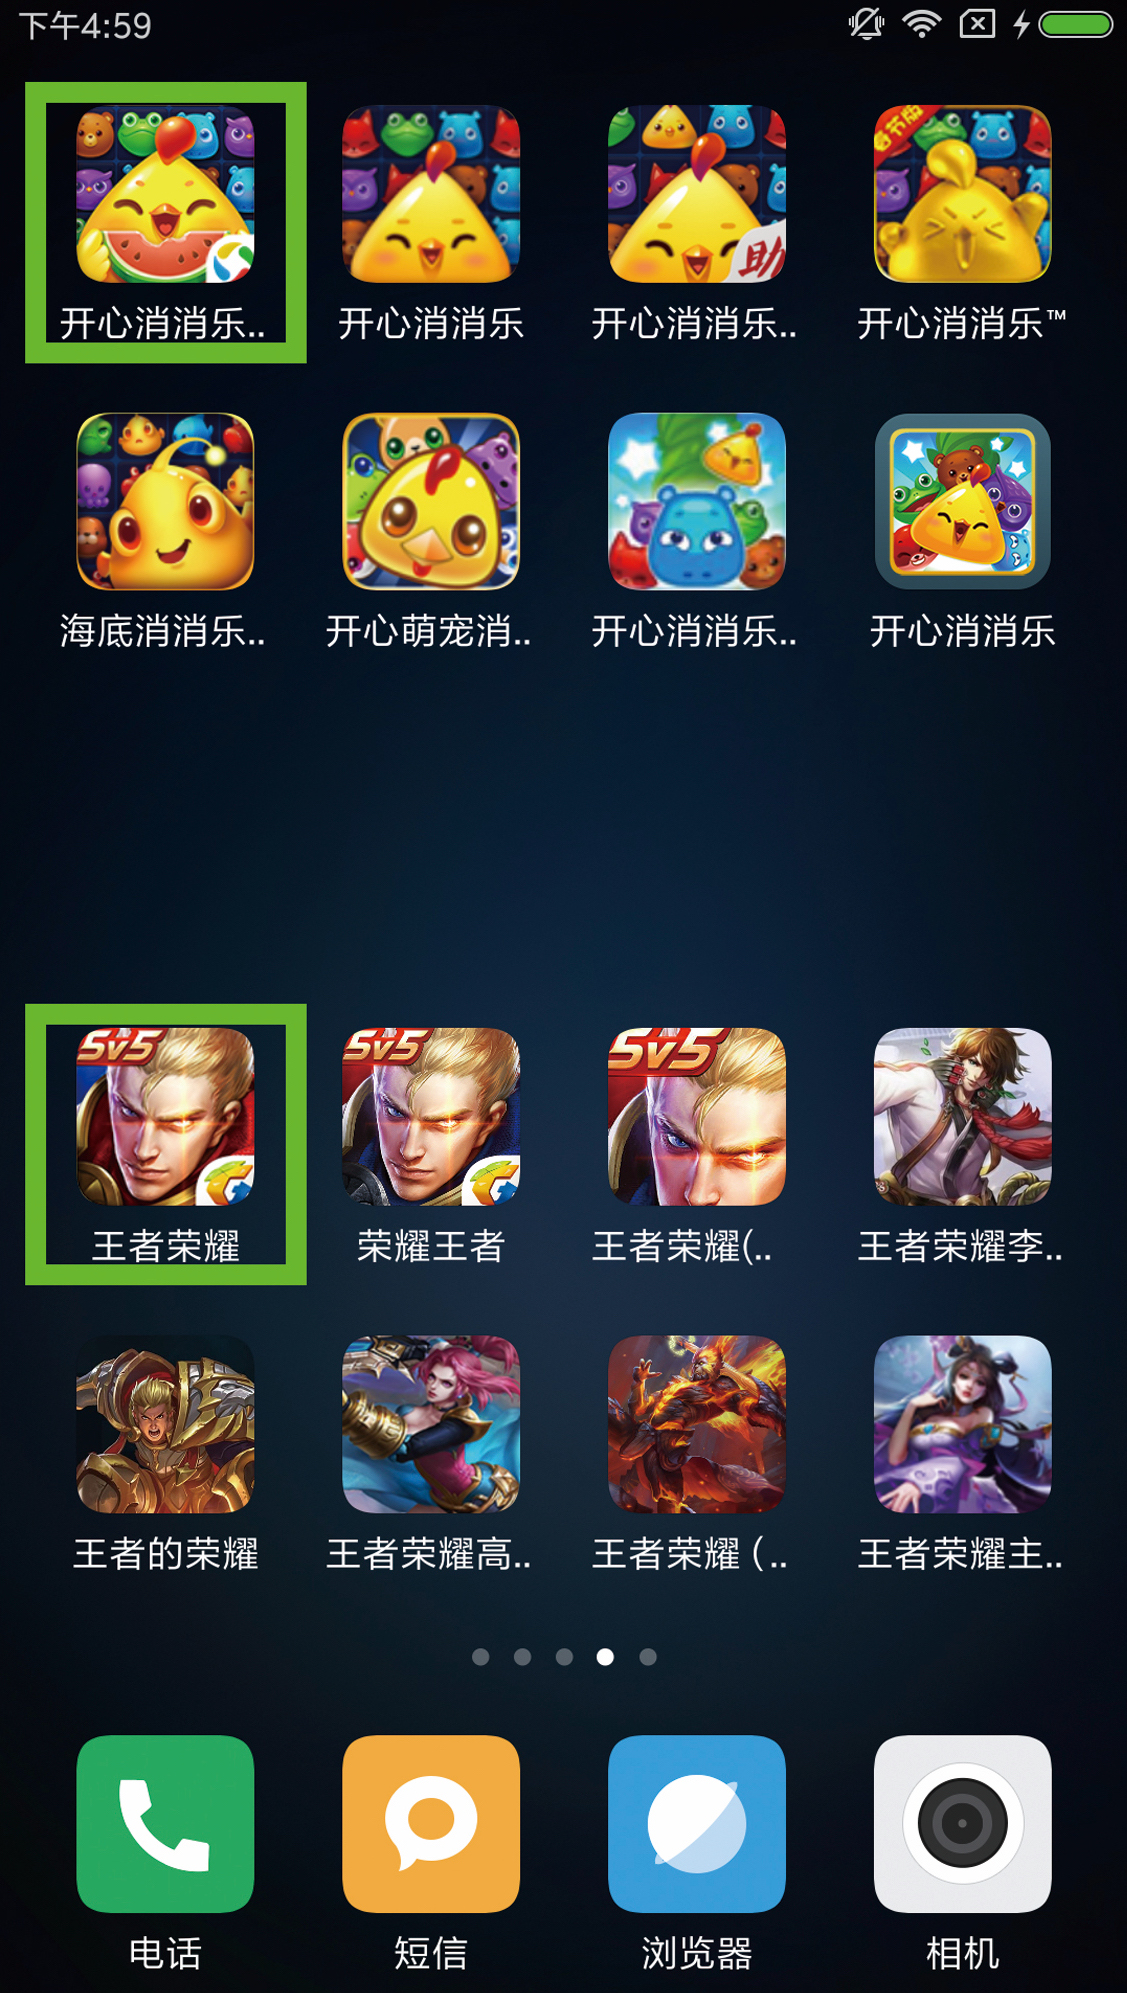
\includegraphics[width=0.3\textwidth]{./Figures/edwin-screenshot1.jpg}}\hfill
    \subfloat[正版\textit{\small 开心消消乐}\label{fig:screenshot_official}]{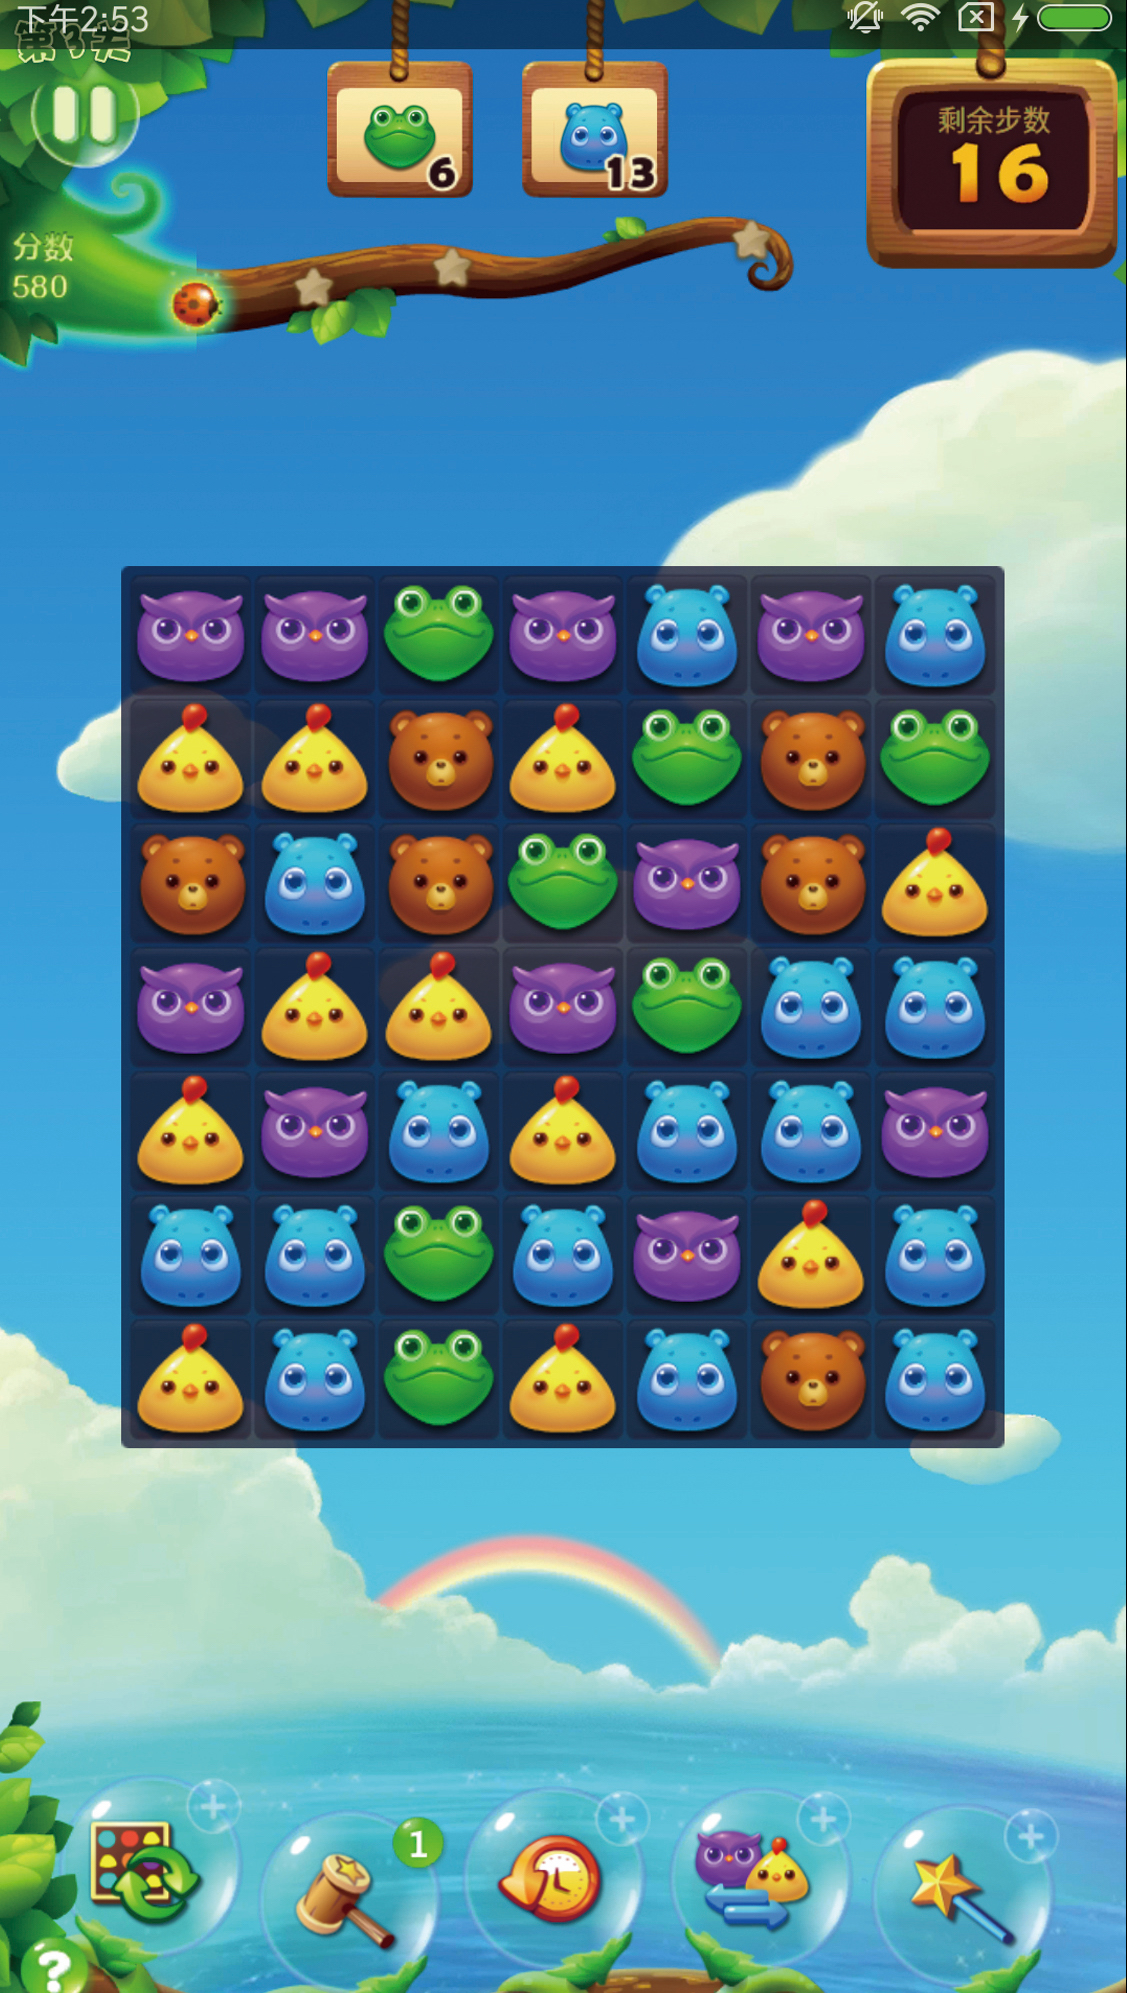
\includegraphics[width=0.3\textwidth]{./Figures/edwin-screenshot2.jpg}}\hfill
    \subfloat[仿冒版\textit{\small 开心消消乐}\label{fig:screenshot_fake}]{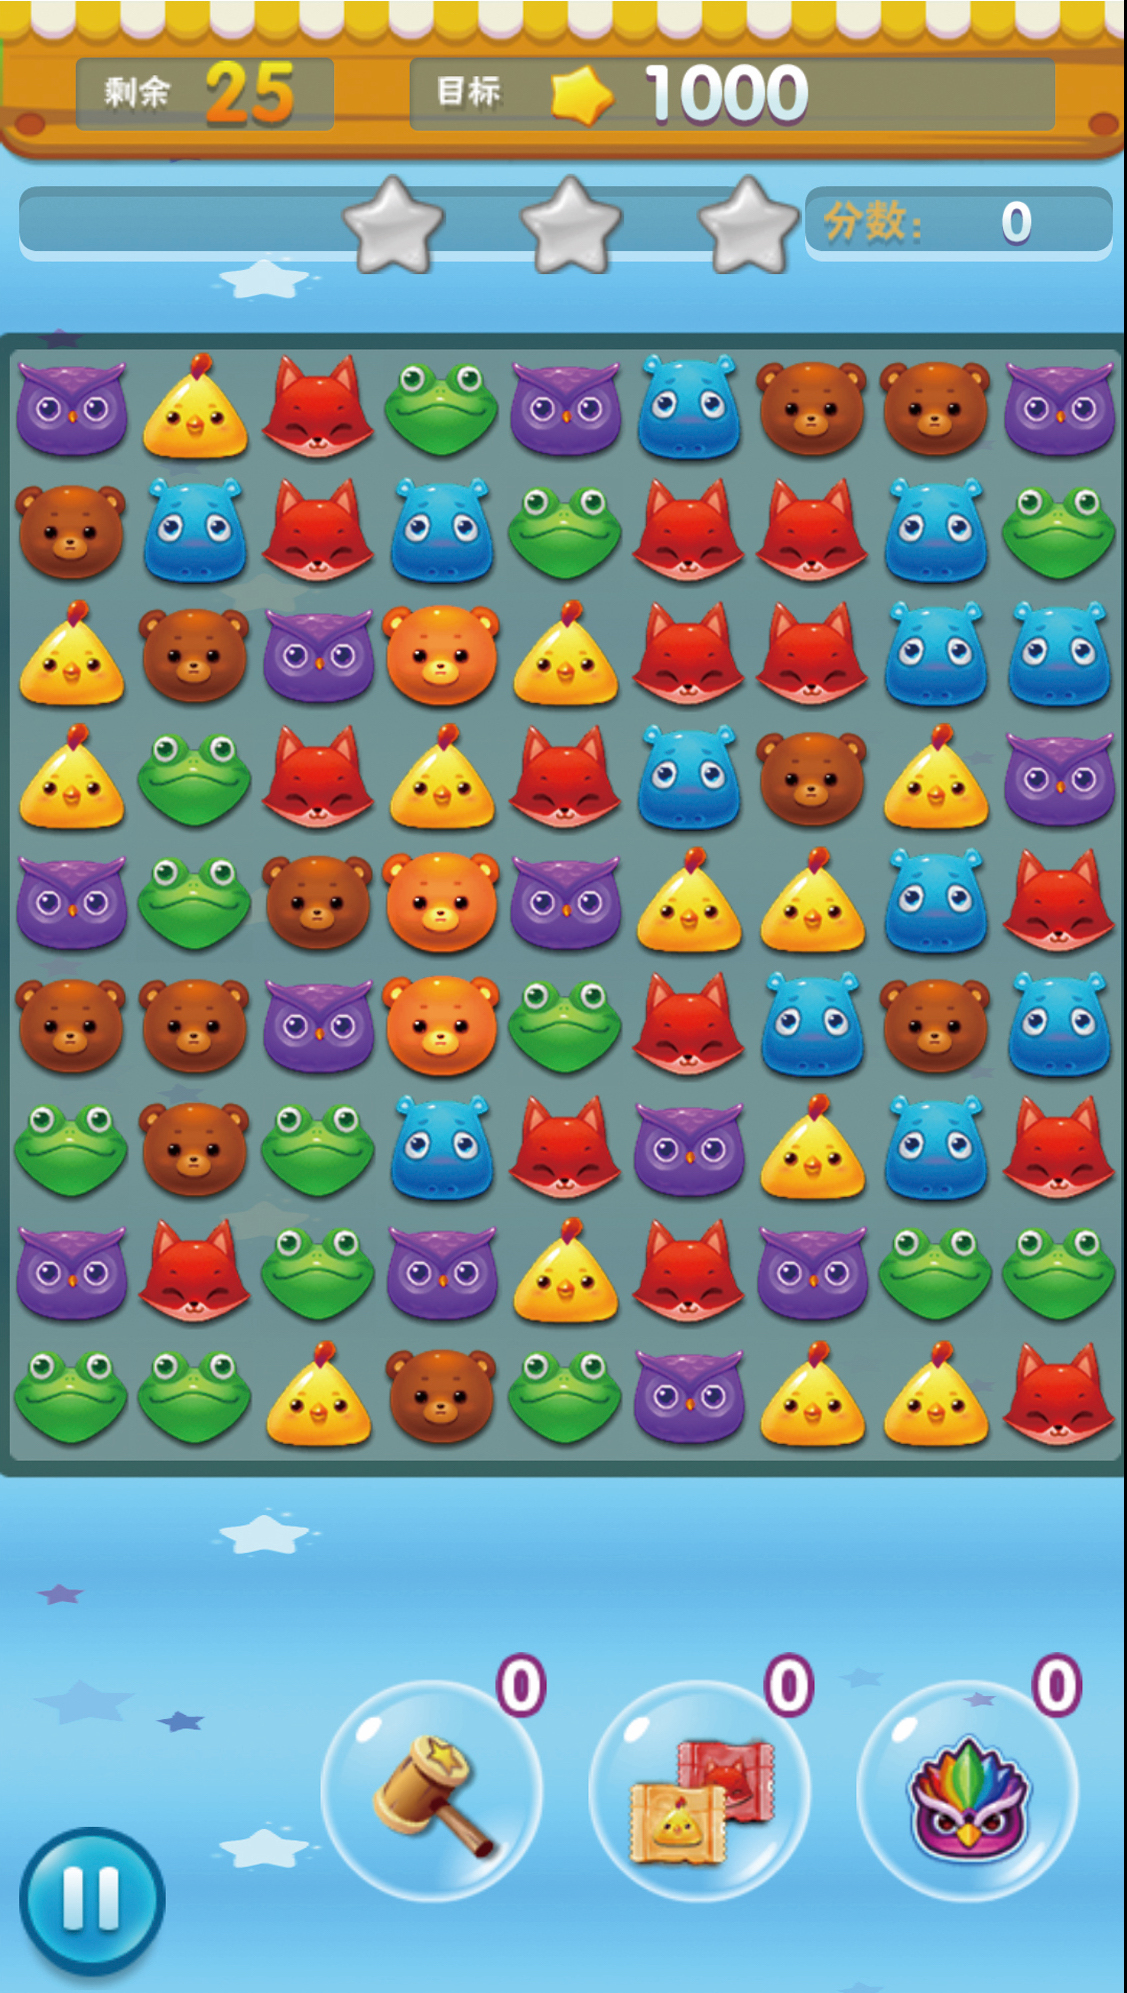
\includegraphics[width=0.3\textwidth]{./Figures/edwin-screenshot3.jpg}}\hfill
    \caption{游戏类App及其仿冒样本}
\end{figure}

\autoref{fig:screenshot_official}和\autoref{fig:screenshot_fake}分别是在测试设备上运行官方版本的\texttt{开心消消乐}和其中一个仿冒版的\texttt{开心消消乐}时的系统截屏。
从UI布局上看,两款应用的外观十分相像。
同时,仿冒版的确实现了完整的游戏功能,与正版的玩法、实际操作逻辑一模一样,有较强迷惑性。
应用开发者未必可判别两个应用的真伪,应用市场的普通用户更难以区分两者。

7款\texttt{开心消消乐}的仿冒样本中,4款与官方样本十分相似(其中之一可能是经过重打包技术处理的应用),2款声称自己是``系统攻略'',1款在运行时闪退,无法在测试设备上实际运行。
在4款仿冒游戏中,3款都在游戏中不时自动弹出游戏内购窗口,要求玩家购买道具,十分可能导致玩家不想要的花费。
所有7个仿冒样本都在\textsc{Virustotal}中被报告为恶意应用。

另一方面,\texttt{王者荣耀}的仿冒样本功能截然不同。
7款仿冒样本中,3款是壁纸浏览器,内含游戏人物插画,可在应用内将插画设置为系统壁纸;
余下4款是简单的拼图游戏,同样包含游戏人物的插画,应用内容为把被打乱的插画拼图恢复原状。
\textsc{Virustotal}显示,7款仿冒样本中,有6款是恶意软件,涵盖了木马病毒、广告软件等类型,而余下的一款则被报告为PUP(Potentially Unwanted Program,潜在有害程序)。
PUP通常在用户不知情或者不愿意的情况下,通过静默安装或者捆绑安装的形式被安装在系统中。
该类软件不一定包含恶意代码,但动机存疑。

造成该现象的原因为模仿正版应用功能难易程度不一。
从技术角度看,\texttt{王者荣耀}的设计、实现难度均比单机益智类游戏如\texttt{开心消消乐}高许多。
多人在线竞技游戏物理引擎之外,还要实现聊天系统、在线匹配、负载均衡等业务模块;
相比之下,益智类游戏的核心逻辑较为简单,无需设计多个复杂模块。

因此,即使不考虑维护问题,开发复杂游戏的成本对仿冒应用开发者而言也明显过高。
但由于\texttt{王者荣耀}的高热度可能带来巨大收益,仿冒应用开发者会为了蹭上热度而开发外观相似、内容完全不符的仿冒样本。
相比之下,\texttt{开心消消乐}由于开发难度相对较小,仿冒应用开发者可开发一个内容相似的应用,再通过内购陷阱等手段收取效益。
这两款应用的仿冒样本透露出了仿冒应用开发者在仿冒方面两个截然不同的思路。

结果前文结果分析,\secref{sec:quantitativeStudy}中显示\texttt{商务办公}类别仿冒率较低也可能是类似原因导致的结果。
一方面,\texttt{商务办公}类的工具核心逻辑比较复杂,仿冒应用开发者不会制作与其功能接近的仿冒应用;
另一方面,该类应用也不像\texttt{游戏}类应用可衍生出周边产品(如\texttt{王者荣耀}的游戏人物插画),仿冒应用开发者无法从周边入手蹭热度。
结合两个原因,\texttt{商务办公}类应用相对不受仿冒应用开发者欢迎。

\subsection{研究结果有效性分析}

结构有效性已于~\autoref{sec:measure_selection}解释,不再赘述。
内部有效性方面,一个可能的威胁是应用与市场之间的关系对该应用在市场上仿冒应用数量的影响。
本章在研究中提出了该可能性,并对相关应用单独进行了进一步检查以消去该因素可能带来的干扰。
外部有效性威胁主要在于实验中仅使用了50款目标应用作为数据,结论可能存在偏差。
的确,50款应用并不能代表Android应用生态的全貌,但市面上的Android应用无穷无尽,收集全量应用进行分析并不可行。
本研究采用的50款应用为国内最受欢迎的50款应用,分别源于11个类别,有一定市场影响力与较大用户群体,本身具有一定代表性与普遍性。
在衡量实验开销与结果有效性后,作者认为选用该组数据进行分析是可行的。

\section{相关工作}

仿冒应用在移动应用行业中早已存在,但少有学者关注仿冒应用的特性。
在已知文献中,与本章研究较为类似的是Khanmohammadi等人对重打包应用进行的实证研究~\cite{khanmohammadi2019empirical},文献中采用了2,776款原版应用和与其对应的15,296个重打包样本作为实验数据,来源为AndroZoo数据集~\cite{li2017androzoo++}。
AndroZoo数据集应用来源是以Google Play市场为主的18个数据源,其中包含4个国内应用市场。
一方面,本研究的数据来源共有29个,以国内市场为主,可更好地反映国内应用市场的现状。
另一方面,本研究虽然只选取了50款原版应用作为对比目标,但收集到的对应仿冒样本有62,638个,对比该文献,每款原版应用都有更多仿冒样本作为研究对象提供数据。
因此,作者认为本文的分析结果更为准确。
再者,该文献仅对重打包应用进行探索,忽视了仿冒应用开发者重新开发相似应用的可能性。
结合前文结果可知,重打包应用在仿冒应用中占比并不高,因而本文提供的结果应更具参考性。


\section{本章小结与实用建议}

本章从三个不同角度对仿冒应用的基本特征进行了实证研究,研究结果可概括如下:
从相似度角度分析,由于仿冒应用开发者目的为诱导用户从应用市场中下载仿冒应用,在用户可感知的方面(应用名),仿冒应用与原版应用相似度较高;在用户较难感知的方面(应用包名与APK大小),仿冒应用与原版应用相差较大。
从影响应用受仿冒程度角度分析,从应用市场规模并不能与应用商店的仿冒率相对应,仿冒应用普遍存在,但应用本身与市场的关系会影响市场中对应的该应用仿冒样本数量;同时,应用的更新频率、热度、类别三个因素均不对应用受仿冒的严重程度起决定性影响,说明应用受仿冒的严重程度是较为复杂的、多因素共同作用的结果。
从仿冒应用可提供功能的角度分析,研究利用案例分析方法,从游戏类别的仿冒应用入手,揭示了仿冒应用开发者对不同应用会采用不同仿冒策略。
对结果进行推断,可以得出``仿冒应用作者更倾向重新制作仿冒应用,而非通过重打包方式制作仿冒应用''的结论。

针对本章实证研究过程的发现,有几点实用建议如下:
1)应用市场方应加强审核流程,除审核应用内容外,也应从外观、应用名、应用内UI等方面对应用进行审核,从源头抵御仿冒应用,保护原版应用作者利益;
基于案例分析可得,仿冒应用包含恶意行为的可能性较大,应用市场方可在该方面加强管理,拦截仿冒应用。
2)应用开发者可更积极地与应用市场方联系,督促应用市场对自身应用的监管。
3)普通用户在搜索、下载应用时,应小心从搜索结果中选择,可结合其他信息(如应用截图、开发者信息)对搜索结果进行判断,避免下载仿冒应用;
也可参考本研究获取正版样本的方法,直接从应用官网下载原版应用安装。
\clearPaperPage

\chapter{仿冒开发者行为特征实证分析}
\label{chp:discoveries_behavior}

本章针对仿冒应用开发者的行为特征进行实证研究,内容主要针对仿冒应用开发者在各市场的投放频率、仿冒应用的投放方式等行为进行研究,了解该类行为有助于市场方与一般应用开发者对抵御仿冒应用作者的攻击。
本章实证研究从三部分展开,结合应用证书视角与结合时间维度视角对仿冒应用开发者的行为进行分析,对应以下三个研究问题:

\begin{itemize}
    \item RQ4:仿冒应用与开发者的对应关系如何?
    \item RQ5:仿冒应用证书可以活跃多长时间?
    \item RQ6:仿冒应用的投放是否有规律?
\end{itemize}

\section{研究方法}

本节介绍本章研究中整理研究数据的方法,以讨论研究的结构有效性。
对RQ4,根据~\autoref{sec:signature}的介绍,可利用样本的应用证书构建其与应用作者的对应关系,RQ5亦涉及应用证书相关信息使用,因此需要阐明应用证书数据的获取方式;
同时,RQ5有对应用证书活跃时间的需求,本章研究引入了一个应用证书活跃时间的近似计算方法;
对RQ6,为研究仿冒引用的投放规律,本研究整理复原了各款正版应用各版本上架的时间线,本节将介绍时间线的整理方法。
本章研究对象为与上一章相同、由69,414个正版样本与52,638个仿冒样本组成的应用集。

由~\autoref{sec:signature},可知每个APK文件内都有包含应用开发者信息的\textit{CERT.RSA}文件。
每个仿冒样本,作者将其解压,取出\textit{/META-INF}文件夹中的应用证书文件,再利用Keytool~\cite{keytool}工具获取证书指纹(即\textit{应用证书SHA1码})。
Keytool工具为Java自带工具,被广泛地用于管理密钥和证书,因此可相信使用Keytool获取的应用证书SHA1码无误。

在获取应用证书活跃时间方面,由于Janus类似一个爬取各大市场应用的平台,并不能感知某样本的下架时间或某样本是否已下架,因此只能对仿冒应用证书的活跃时间作近似计算。
计算的具体方法为将所有仿冒样本遍历一次,取出样本的应用证书SHA1码,凭借该样本的搜集时间更新该应用证书的最早出现时间(或最晚出现时间),取各证书最早出现时间与最晚出现时间为证书的活跃期,活跃期长度则为该证书的活跃时长。

为了解仿冒应用的投放速度,研究需要获取各款目标应用每个版本的更新时间和与该版本对应的仿冒样本的上架时间。
各个目标应用多年来发布版本众多,已无法从大部分应用官网中寻回完整更新日志,因此本研究借助样本集中的正版样本搜集时间整理复原各版原版应用的上架时间线。
本文对所有收集到的正版样本按目标应用进行分类,再按照版本号对同一目标应用下所有样本排序。
由于同一应用可在多个市场上架,同一版应用在不同市场可能存在细小差别(如在华为市场上架的应用需要接入华为钱包作为支付途径),导致同一版本的APK安装包具有不同SHA1码,因此此处以应用版本而非应用SHA1码为粒度分割样本,以消除上述情况影响。
另外,基于各市场审核流程、其他商业因素考虑,可能存在应用同一版本在不同市场有不同上架时间的情况。
针对该情况,如某版原版样本存在多个上架时间,本研究只取最小值,该值表示仿冒应用开发者可接触该版原版应用的最早时间。
之后,将每款应用中每个版本上架时间串联,即可大致重现每款应用的更新时间线。


从仿冒样本角度考虑,仿冒样本大多不是重打包应用,无法与原版应用的版本号直接对应。
为求出仿冒样本的仿冒延迟(即原版应用上架时间与仿冒样本上架的时间差),本文提取出每个仿冒样本的上架时间,以不晚于这个仿冒样本发布的原版应用作为其对应的仿冒对象,取两者上架时间差作为仿冒延迟。

% % \noindent{\bf Hypo 1.1:} Most of these fake samples have their corresponding unique certificates.
% {\bf 假设 1.1}: 绝大部分的仿冒样本有其对应的、独一无二的安全证书。
% % In other words, most fake certificates and fake samples have a one-to-one relation.
% 即绝大部分仿冒应用和他们的安全证书呈一对一的映射关系。

% 与之对应,本文提出了以下的研究问题:

% % \noindent{\bf RQ 1.1}: What's the relationship between the number of fake samples and their certificates? That is, how many fake samples does one certificate usually link to?
% {\bf RQ 1.1}:仿冒样本数量和他们的安全证书数量存在着什么样的关系?也就是说,一个安全证书通常会跟多少个仿冒应用样本相关联?

% 为了解答这个问题,本文从所有搜集到的样本中提取出安全证书,然后对这些证书和样本做了配对。
% 根据配对得出的数据,本文得出了以下结果:

% % \noindent{\bf Answer to RQ 1.1.}
% {\bf RQ 1.1. 结果}
% % 76\% of these fake certificates are linked to merely one or two fake samples, and the number of fake examples a certificate links to is various from 1 to 1,374.
% 在仿冒应用持有的所有安全证书中,76\%都仅仅关联到了一到两个仿冒样本,与单个安全证书相关联的仿冒应用数分布在从1到1,374的区间内。
% % We count the number of certificates which link to different sample number in table~\autoref{table:certificate_number_statistic}.
% \autoref{table:certificate_number_statistic}统计了安全证书和他们对应的仿冒样本数量。
% 其中第一栏为仿冒样本的数量区间,第二栏为关联的仿冒样本数量该落于区间的安全证书数。
% 大部分安全证书都只关联了1到5个应用样本,但也有少量安全证书与大量仿冒样本有关联关系。

% \begin{table}[htbp]
%     \renewcommand{\arraystretch}{1}
%     \footnotesize
%     \centering
%     \caption{安全证书/仿冒应用数量对应表}
%     \vspace{1mm}
%     \begin{tabular}{l c c c c c c c}
%         \toprule
%         {\bf 仿冒样本数量} & {\bf 1-5} & {\bf 6-10} & {\bf 11-50} & {\bf 51-100} & {\bf More than 100} \\
%         \midrule
%         {\bf 安全证书数量} & 8252      & 525        & 531         & 71           & 80                  \\
%         \bottomrule
%     \end{tabular}
%     \label{table:certificate_number_statistic}
% \end{table}

% % This discovery partly matches our assumption that most of these fake samples have their corresponding unique certificates.
% 这个发现与本文的猜想(即大多数仿冒样本都有他们对应的独一无二的安全证书)部分相符。
% 虽然并不是大多数仿冒样本都有其单独对应的安全证书,但多数安全证书的确只对应少量样本。
% % We consider this as a strategy to bypass app markets' security scheme, as even if one fake sample is exposed, other fake samples developed by the same developer will not be implicated directly.
% 结合\secref{sec:signature}Android App签名机制最后的说明,本文认为这是规避应用市场监管机制的一个策略。
% 如果以同一开发者的身份,用一个安全证书上传多个仿冒App,万一其中App被投诉下架,其他的App很可能会受到牵连。
% 然而,一个仿冒开发者其实也可以持有多个安全证书。
% 如果使用多个安全证书分别上传仿冒App,应用市场就不容易找到这些App的关联,即使其中一部分被举报下架,余下的也得以被保全。
% % Nevertheless, when reviewing certificates linked with multiple fake samples, we find some very surprising findings that we will expound in Section~\autoref{sec:casestudy}.
% 另外,在整理对应多个仿冒样本的安全证书时,本文得到了一些意料之外的发现。相关内容会在后续案例分析中加以拓展。


% \vspace{5mm}
% \noindent\fbox{
%     \parbox{0.95\linewidth}{
%         % \textbf{Remark 1}: Most certificates link with only a number of fake apps, which is highly possible to be a fake developers' evasive strategy.
%         \textbf{本节小结}: 绝大部分安全证书只与少数仿冒样本有所关联。这很可能是仿冒开发者规避市场监管机制采用的策略。
%         % Moreover, we observe that fake apps do tend to use official app names or names alike.
%         同时,本文也观测到仿冒应用倾向于于官方App相同或者是十分相似的应用名。
%         % Nonetheless, fake apps and official apps are not resemble in terms of package names or apk sizes, disclosing that repackaged apps are not mainstream in fake apps.
%         但是,仿冒样本和官方App在包名和APK包大小方面都不相似,这表明重打包应用在仿冒应用中并不普遍存在。
%         最后,如果良性应用的开发者不遵从最新的安全标准发布应用,可能会导致十分严重的安全问题。
%     }
% }

% % We manually review the samples signed by the certificate with SHA1 ``\emph{61ed377e85d386a8dfee6b864bd85b0bfaa5af81}", the certificate with the most number of fake samples among our fake certificate set (i.e., 1,374 fake samples).
% \secref{sec:fakeCharacteristics}提到有部分仿冒应用安全证书关联着多个仿冒样本。
% 其中,一个SHA1码为``\emph{61ed377e85d386a8dfee6b864bd85b0bfaa5af81}''的安全证书是所有证书中关联仿冒样本最多的,足足有1,374个样本持有这个仿冒证书。
% % On top of that, this certificate is also one of the certificates survive the longest time (nearly 3 years) and is still active.
% 不仅如此,这个安全证书还是其中一个在应用市场中活跃时间最长的仿冒应用安全证书。
% 它的出现横穿了本研究的整个研究时间过程(接近三年),而且在本研究的数据收集流程结束前依然呈现活跃状态。

% % Originally, we presume this certificate to belong to a benign app which passes the verification of analysts in Pwnzen, since the number of samples it links to even exceeds the number of official samples of some apps.
% 最初,本研究假定这个证书属于某个通过犇众分析团队验证的良性应用,因为它关联的样本数量实在是太大了,这个数量甚至超过了本研究中某些目标App的样本总量。
% % The truth is, however, after manually review, we found all the 1,374 samples linked with this certificate are typical fake samples, in form of either imitators or imposters, covering 79\% (37 out of 47) of our target apps.
% 然而在人工审核之后,本研究却有意料之外的结果。
% 这个证书关联的所有1,374个样本都是典型的仿冒样本,其中既有只与原版应用稍微近似的\texttt{模仿应用},也有外观上完全模仿原版应用的\texttt{高仿应用},覆盖了本研究能找到的47个目标App中的37个(79\%)。
% % Some of its samples can even be organized in version order, which means the developer does track official apps to update its fake versions as maintenance.
% 而这些证书关联的一些样本,甚至有自己的版本顺序,这表明有的开发者真的会追踪官方App的各个版本来更新、甚至维护自己的仿冒版本。

% \begin{table}[htbp]
%     \renewcommand{\arraystretch}{1}
%     \small
%     \centering
%     \caption{由``61ed377e85d386a8dfee6b864bd85b0bfaa5af81"签署的部分样本}
%     \vspace{1mm}
%     \rowcolors{2}{gray!15}{white}
%     \begin{tabular}{l l c c c c c c}
%         \toprule
%         {\bf 应用名} & {\bf 包名}                     & {\bf 大小} \\
%         \midrule
%         QQ Talk      & net.in1.smart.qq               & 465.8 KB   \\
%         QQ           & com.h                          & 8.2 MB     \\
%         爱微信       & com.lovewechat                 & 368.4 KB   \\
%         微信         & com.tencen1.mm                 & 22.1 MB    \\
%         UC Mini      & com.uc.browser.en              & 2.1 MB     \\
%         UC 浏览器    & com.UCMobile.microsoft         & 21.3 MB    \\
%         Clean Master & com.blueflash.kingscleanmaster & 972.0 KB   \\
%         WiFi万能钥匙 & com.snda.wifilocating          & 5.9 MB     \\
%         \bottomrule
%     \end{tabular}
%     \label{table:certificate_case_study}
% \end{table}

% % We display some of the samples singed by this certificate in Table~\ref{table:certificate_case_study}, they are all reported to be malicious (i.e., Ad-ware, spyware or Trojan) on \textsc{Virustotal}~\cite{virustotal}, a famous online antivirus engine.
% 本文在\autoref{table:certificate_case_study}中展现了由这个安全证书签署的部分样本。
% 这批样本随后被上传到知名在线反病毒引擎\textsc{Virustotal}~\cite{virustotal}上。
% 结果显示,与该证书关联的所有样本都是恶意样本(广告软件、间谍软件或木马软件等)。
% % So far the samples related to our target apps have already been showing up in 20 markets including the leading ones like \texttt{\small Myapp} and \texttt{\small Qihoo 360 Market}.
% 到目前为止,由这个证书签署的仿冒样本已经在本研究的20个应用来源(即应用市场)中出现,包括\texttt{应用宝}和\texttt{360应用市场}等主流应用市场。
% % What's more, \texttt{\small Baidu App Store} keeps receiving apps with this certificate from 2015 to recently -- its latest ``product'' was put on shelf on September 15$^{th}$, 2018.
% 除此之外,\texttt{百度手机助手}从2015年起就开始接受由这个安全证书签署的应用,直到本研究的数据收集阶段结束前——数据显示,这个安全证书在2018年9月15日还在\texttt{百度手机助手}上架了一款应用。

% % To this end, we can draw the following conclusions:
% 在这里,可以得到以下两个结论:
% \begin{itemize}
%     % (1) Even the leading app markets (and the top developers) are unqualified in detecting malicious apps.
%     \item 就算是领先的应用市场(和顶尖的开发者)在检测恶意应用方面也不能做到尽善尽美,而现有的检测方法也有所不足,未能及时地找出可疑的开发者;
%           % (2) Existing app markets lack information exchange on defending attacks from underground industry.
%     \item 从这个证书在多个市场都存在的现象,本研究推导,现有的应用市场缺乏有效的信息交换机制。
%           如果各个应用市场能建立一个互通信息的平台,分享可疑开发者/恶意开发者信息,那么将可以杜绝一部分恶意开发者在各个应用市场上到处流窜的现象。
% \end{itemize}


% \section{实证研究流程与结果解析}

% 本节分为四个部分,前三个部分分别对应本章三个研究问题的研究流程,最后一部分对本章研究进行有效性分析。

% \subsection{应用证书与仿冒应用对应关系}

% \subsection{仿冒应用证书活跃时长}
% 从某个角度看,仿冒应用安全证书的活跃时长反映了应用市场的监管力度大小,也能反映市场之间在安全方面是否具有良好的合作机制。
% 所以本节有研究问题如下:

% % \noindent{\bf RQ 3.2} How long can a fake app's certificate survive?
% {\bf RQ 3.2}:一个仿冒应用开发者的安全证书可以活跃多久?

% 本文整理了不同仿冒应用安全证书的出现时间,得出了下面的结果:

% % \noindent{\bf Answer to RQ 3.2.} Fig.~\autoref{fig:Fake_certificate_survival_distribution} shows the distribution of the time a fake certificate can survive in markets.
% {\bf RQ 3.2. 结果}\autoref{fig:Fake_certificate_survival_distribution}展示了不同仿冒应用安全证书在应用市场里活跃时间的总体分布。
% % In the left density distribution subplot, $x$-axes is the latency and $y$-axes shows the probability density of data at corresponding $x$ value.
% 在左边的密度分布函数图中,$x$轴表示其活跃的时长,$y$轴则表示了与$x$轴上的值对应的概率密度。
% % The total area under the curve is 1, and the area under two $y$ values $y1$ and $y2$ is the probability of their corresponding value $x1$ and $x2$ account for in data.
% 曲线下的总面积为1,任意两个$y$值$y_1$、$y_2$之间的曲线下面积是其对应的$x$轴上的值$x_1$、$x_2$在数据中占有的概率。
% % For example, in Fig.~\autoref{fig:Fake_certificate_survival_distribution}, the area beneath curve between 0 to 200 on $x$-axes is close to 0.8, which means nearly 80\% of certificates only survive for no more than 200 days.
% 比如说,\autoref{fig:Fake_certificate_survival_distribution}中$x$轴从0到200之间的值对应的$y$轴曲线下方的区域面积接近0.8,意味着约80\%的仿冒应用安全证书不会活跃多于200天。

% % To judge how long a fake certificate can survive is similar to how we calculate the update frequency of an app, the first time and the last time a fake sample from the same certificate gets crawled are marked.
% 断定一个仿冒应用安全证书活跃市场的方法和前述计算应用更新频率的方法稍有类似,本文把某个安全证书关联的所有样本都找出来,提取出其中最早和最晚被爬取的样本的发布日期时间戳,然后将他们的差值的绝对值当作是这个安全证书的活跃时长。
% % The time when a sample was crawled from a market might be different from the time when it is available in the market, but our crawler downloads new samples from different markets by days and we also use days as the unit in our measurement, so we can approximately regard this two values as the same one.
% 从时长上爬取到样本的日期与样本在应用市场上实际能活跃的时间稍有不同,但由于Janus的爬虫工具每日都从应用市场中爬取样本,而本文并没有其他方法可以知晓某款App具体在应用市场中上架了多久,只能近似地将上述提到的时间差当作是某个安全证书能在应用市场上活跃的时间。

% \begin{figure}[htbp]
%     \centering
%     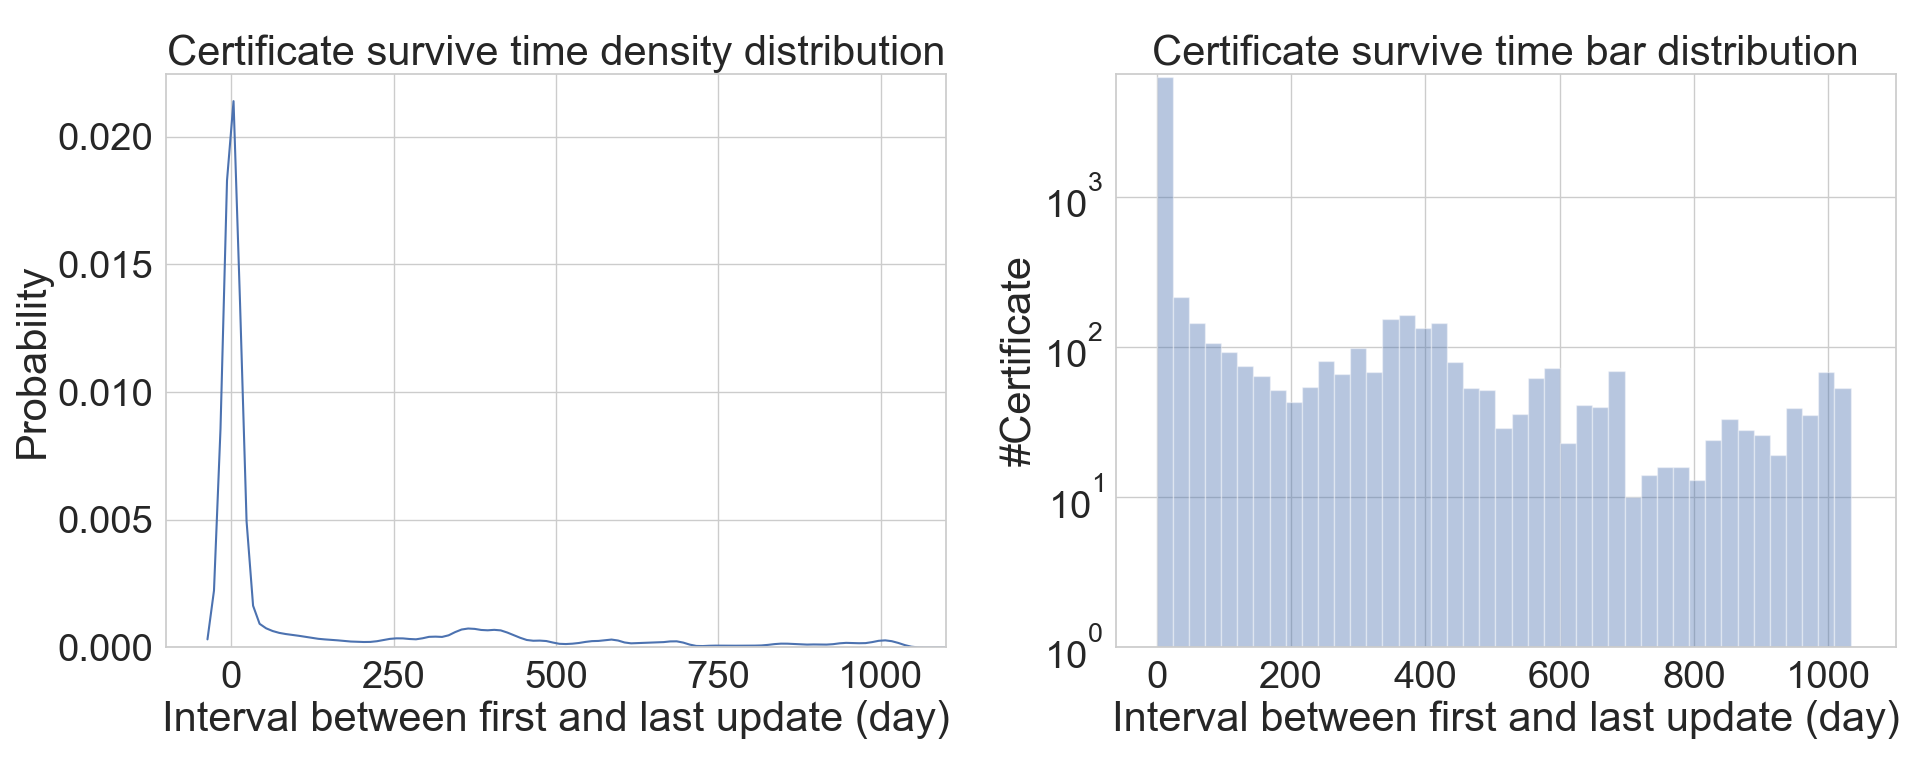
\includegraphics[width=\textwidth]{./Figures/edwin-Fake_certificate_survival_distribution2.png}
%     \caption{仿冒应用安全证书活跃时间分布}
%     \label{fig:Fake_certificate_survival_distribution}
% \end{figure}

% % As shown in Fig.~\autoref{fig:Fake_certificate_survival_distribution}, the distribution of fake certificate survival time shows that almost all the fake certificates live a short life, which means most fake certificates only show up in a short period of time.
% 正如\autoref{fig:Fake_certificate_survival_distribution}所示,仿冒应用安全证书活跃时间的分布表明几乎所有仿冒应用安全证书都只能活跃相当短的时间,这表明大多仿冒应用只会在一个很小的时间窗口里出现,然后迅速消失。
% % This can be explained by a scheme that most markets have.
% 这可以由大部分市场都有的一个安全机制解释。
% % Once an app is found malicious or illegal, the market would stop that specific developer from uploading more samples by refusing to receive samples with the same certificate.
% 只要一款App被发现具有恶意行为或者违法行为,应用市场就会禁止开发者再使用该证书上传应用,也就是常见的封号处理。
% % There are also a number of certificates which can survive for a long time.
% 但是,也有一部分的仿冒应用安全证书活跃了相当久的一段时间。
% % According to the figure, some fake certificates even traverse the whole study interval.
% 根据图表信息,可以看到有的仿冒应用安全证书的生命周期甚至贯穿了本文整个研究截取的时间周期。
% % We will conduct a case study on this phenomenon in Section ~\autoref{sec:casestudy}.
% 对于这个异常样本,本文会在后续的案例分析中有更详尽的案例分析。

% \begin{figure}[htbp]
%     \centering
%     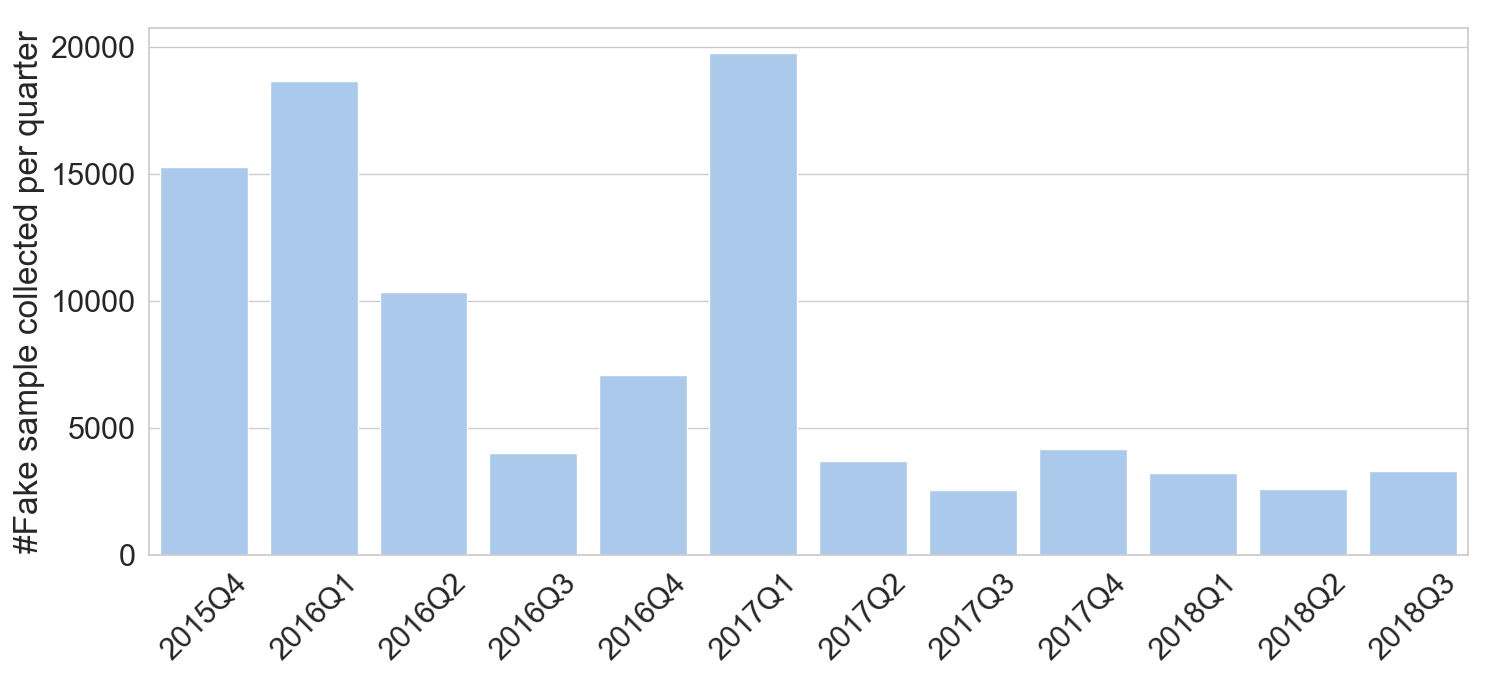
\includegraphics[width=\textwidth]{./Figures/edwin-Number_of_samples_collected_per_quarter_3.png}
%     \caption{每季度爬取到的仿冒样本数量(2015年第四季度到2018年第三季度)}
%     \label{fig:Number_per_quarter}
% \end{figure}

% \subsection{仿冒应用投放规律分析}
% 在正版应用推出新版后,如果一个仿冒应用能在越短时间内推出对应的新版本,仿冒应用的开发者就越有可能蹭上软件更新的热度,从而获利。
% 对此,本节提出了以下研究问题:

% % \noindent{\bf RQ 3.1} After a new version of an official app is published, how long do fake developers take to publish a new fake sample? In other words, how soon will these copycats appear?
% {\bf RQ 3.1}:在一个官方应用的新版本推出之后,仿冒应用开发者需要花多少时间去推出对应版本的仿冒版?
% 换句话说,这些``山寨''版本会过多久出现?

% 在分别复原官方应用的更新时间线和对应仿冒版本的发布时间之后,本文得到了以下结果:

% % \noindent{\bf Answer to RQ 3.1.}
% {\bf RQ 3.1. 结果}
% % We compute this latency and show its distribution in Fig.~\autoref{fig:Fake_latency_overall_distribution}.
% 本文计算出了每版App被仿冒的延迟时间和延迟的分布情况,结果显示在\autoref{fig:Fake_latency_overall_distribution}中。

% \begin{figure}
%     \centering
%     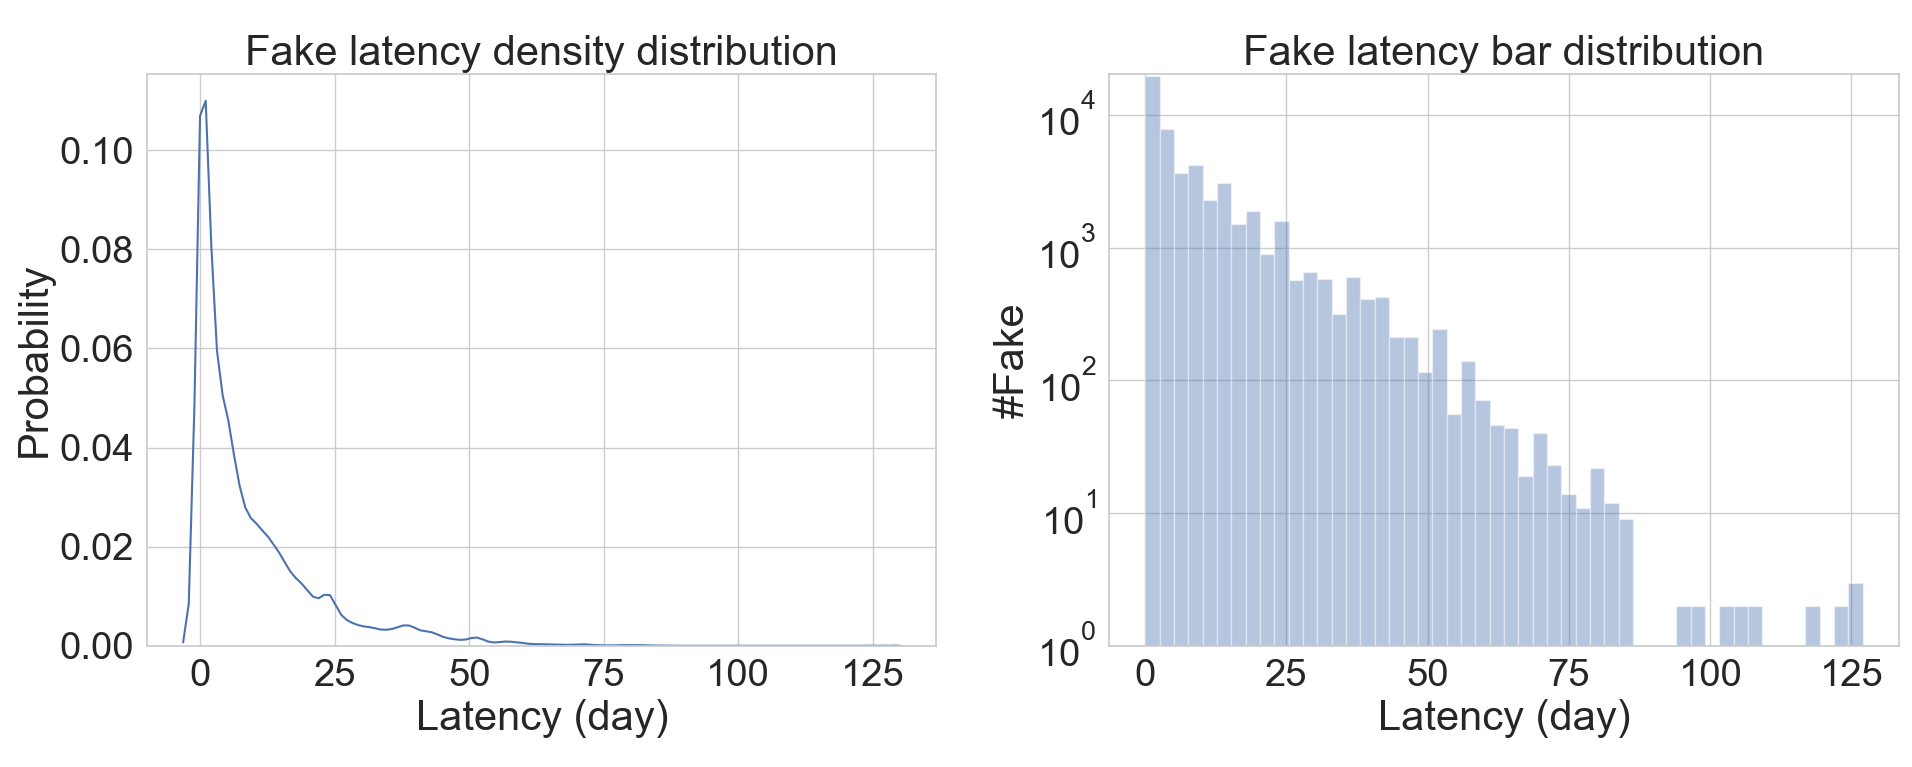
\includegraphics[width=\textwidth]{./Figures/edwin-Fake_latency_overall_distribution2.png}
%     \caption{仿冒延迟总体分布}
%     \label{fig:Fake_latency_overall_distribution}
% \end{figure}


% % Fig.~\autoref{fig:Fake_latency_overall_distribution} shows that most fake samples are published with the latency shorter than 20 days.
% 按照\autoref{fig:Fake_latency_overall_distribution}的结果,绝大多数仿冒样本在官方应用推出后的20天内就被发布了。
% % According to our statistics, 60\% of fake samples show up in 6 days after a new version of the official app is published.
% 根据本文的统计,有60\%仿冒应用在正版App被推出的6天内就被发布出来了。
% % This reveals a truth that fake developers are swift in action.
% 这表明仿冒开发者的行动十分迅速。

% 随着时间推移,仿冒应用这个灰色产业是否有过变迁?
% 本节对此提出了研究问题:

% % \noindent{\bf RQ 3.3} Is there a changing pattern of fake samples over time?
% {\bf RQ 3.3}:仿冒应用是否存在一个随着时间变化的模式?

% 本研究统计了不同时间段所搜集到的样本数量,得出了结果如下:

% % \noindent{\bf Answer to RQ 3.3.} Fig.~\autoref{fig:Number_per_quarter} shows the number of fake samples collected per quarter since the fourth quarter of 2015.
% {\bf RQ 3.3. 结果}\autoref{fig:Number_per_quarter}呈现了Janus自2015年第四季度起在每个季度爬取到的仿冒样本的总量。
% % Although a large number of new fake samples get released in every quarter, the figure shows a tendency that the total number of fake apps on markets is gradually decreasing by years.
% 尽管Janus每个季度都能爬取到新上架的大量仿冒样本,图表信息表明,市场上仿冒应用的总数正在呈现逐年减少的趋势。
% % Note that our statistics only focus on fake samples, consequently this phenomenon does not indicate the underground industry is turning down.
% 要注意的是,此处的统计仅仅针对仿冒应用。
% 因此这个现象并不表明移动黑灰产的发展具有萧条的趋势。
% % Instead, we suppose this is possibly caused by the reform of fake apps.
% 相反地,本文认为这个现象更有可能是由黑灰产内部改革而导致的。

% % On one hand, as stricter review schemes and stronger protection systems are applied on app stores, it's inevitable that fake apps in this study, become harder and harder to get on the shelf.
% 从一方面看,随着信息技术发展,应用市场逐渐配备上了更智能、严格而又强大的监管机制和安全系统,本研究中的仿冒应用开发者无疑更难以将仿冒的应用投放到市场上了。
% % On the other hand, the new generation of malicious software, such as ransomware~\cite{ransomware} is impacting the underground industry.
% 从另一方面看,新一代的恶意软件,比如WannaCry等勒索软件~\cite{ransomware}也正在影响着整个移动黑灰产工业。
% % Compare to fake apps, the new malicious apps are not only hard to defend (due to the innovative or even state-of-the-art techniques they utilize) but also extremely profitable.
% 与仿冒应用相比,这些新一代的恶意软件不仅更难以防范(传统的反病毒软件思路是提取已有恶意代码的特征,从而识别恶意行为,但这无法遏制新型的恶意行为),而且也似乎更容易能获取暴利。
% % Wannacry, a ransomware which was first spotted in the 2nd quarter of 2017, conquered tens of thousands of devices in a couple of weeks, which directly pulled up Bitcoin's price like a rocket~\cite{wannacry_bitcoin_news}.
% Wannacry作为一种新型恶意软件,自2017年第二季度被首次发现开始,就能在数周内攻克数以千万计的设备,并让比特币的价格像搭火箭一样直线飙升~\cite{wannacry_bitcoin_news}。
% % Afterward, in the first quarter of 2018, a burst of cryptomining malware on phones emerged~\cite{comodo_report}.
% 之后不久,在2018年的第一季度,移动设备上也爆发了一系列的加密采矿恶意软件~\cite{comodo_report}。
% % This may be the reason why the number of fake samples suffers two suddenly drops in the second quarter of 2017 and the first quarter of 2018, respectively.
% 所以,本研究有理由猜测2017年第二季度和2018年第一季度的仿冒应用上架数量下跌是受到了新形态黑灰产的冲击。
% 当然,证实这个猜想还需要采集更多数据、进行更深入的研究。

% \subsection{研究结果有效性分析}
% \subsection{案例 1. 持有官方安全证书的可疑样本}

% 在人工浏览数据时,本研究发现了一个具有可疑应用名的样本---该样本声称自己是一个``破解版''的应用。
% % Furthermore, we checked (1) if strange word (e.g., ``cracked") appears in our official samples' names, (2) whether or not an official app is signed by an official certificate from another developer, and (3) if one official sample has a suspicious package name.
% 因此,本研究针对所有69,614个持有官方证书的样本进行了以下筛选:
% \begin{enumerate}
%     \item 使用``破解''、``免费''等关键字搜索所有带正版证书的样本,筛选出带有可疑应用名的样本;
%     \item 筛选所持安全证书与原开发者不一致的样本;
%     \item 筛选出包名和同款App的多数样本不一致的样本。
% \end{enumerate}

% % Eventually we acquired 17 suspicious official samples, listed in table~\ref{table:suspicious_samples} are samples in each of these three kinds.
% 最终,本文获得了17个由正版开发者安全证书签署的可疑样本,其中三个样本的信息如\autoref{table:suspicious_samples}中所示,分别代表上述三项筛选得到的结果。
% 第一个名为\texttt{爱奇艺}的样本虽然由一个官方安全证书签名,但该安全证书和其他爱奇艺样本的却不一致。
% 对比之后,本研究发现该证书来自360手机助手,但360和爱奇艺并没有合作关系,因此这是个可疑的样本;
% 而第二个样本(\texttt{360手机助手})的可疑之处在于样本包名。多数\texttt{360手机助手}的包名为\emph{com.qihoo.appstore},也有少部分官方包名为\emph{com.qihoo.secstore},前者为\texttt{360手机助手}在国内第三方应用市场发行的应用包名,后者为Google Play官方应用市场上上架的包名。然而,其中一个使用了其官方安全证书签署的样本的包名却是\emph{com.kuyou.sdbgj.baidu},十分奇怪;
% 第三个样本则是在应用名中包含了``破解''字样。然而,正常的正版应用根本不会有这样的命名方式,所以本研究也认为这是一个可疑样本。


% % \textsc{Virustotal} reports that only 2 of the 17 samples are benign, 2 are PUP and the other 13 samples are all malicious.
% \textsc{Virustotal} 的检查结果显示,17个可疑样本中,只有2个是良性应用,2个是PUP,余下13个样本都被判定具有恶意行为。
% 进行后续分析时,相关样本已被剔除出正版样本集合。

% \begin{table*}[htbp]
%     \renewcommand{\arraystretch}{1}
%     \small
%     \centering
%     % \setlength{\belowcaptionskip}{-10pt}
%     \caption{持有官方安全证书的可疑样本}
%     \begin{tabular}{l l c c c c c c}
%         \toprule
%         {\bf 样本应用名}               & {\bf 样本SHA1码}                         & {\bf 可疑之处} \\
%         \midrule
%         % 爱奇艺 & b86c55a509e8293b24138b166e9ff410f39e84b5 & 可疑证书(360手机助手) \\
%         爱奇艺                         & b86c55a509e8293b24138b166e9ff410f39e84b5 & 可疑证书       \\
%         % 360手机助手 & 2bb43c53b86d204d0040a8af6cb2a09cf9e93bb7 & 可疑包名(com.kuyou.sdbgj.baidu) \\
%         \rowcolor{gray!15} 360手机助手 & 2bb43c53b86d204d0040a8af6cb2a09cf9e93bb7 & 可疑包名       \\
%         % Youku XL 破解版 & b55b7ef189d649aeb03443c5d1ab57c9031d624e & 可疑应用名(``破解版") \\
%         Youku XL 破解版                & b55b7ef189d649aeb03443c5d1ab57c9031d624e & 可疑应用名     \\
%         \bottomrule
%     \end{tabular}
%     \label{table:suspicious_samples}
% \end{table*}

% % Despite the possibility that these certificates were somehow leaked to the underground industry, it is more likely that some attackers penetrated the protection scheme.
% 鉴于这17个样本都是持有官方安全证书签名的,有理由怀疑有应用厂家不慎泄露了自己的安全密钥库,从而导致了这些样本的出现。
% 然而,如果真的是因为厂家泄露密钥库,一来很有可能会导致恶意开发者使用官方安全证书大量生产恶意应用,二来对应厂家也会出于安全考虑马上更换新的包名和安全证书。
% 本研究的数据并不支持以上猜想带来的两点结果,所以本文不认为这是由于安全证书泄露导致了这些可疑样本的产生。

% 除去这个可能性,本文认为更有可能的原因是某些仿冒应用开发者掌握了穿透/绕过Android系统签名机制的技术,从而产生了这些样本。

% % As far back as December 2017, Google had confirmed and revealed a backdoor on V1 signature scheme (CVE-2017-13156)~\cite{android_security_bulletin}, by which hackers can inject any content into an apk at will without modifying its certificate information.
% 时间回溯到2017年12月,Google确认并公布了V1版本应用签名机制的一个后门(CVE-2017-13156)~\cite{android_security_bulletin}。
% 通过这个后门,黑客可以在不修改APK包安全证书信息的情况下,向APK包里注入任意内容。
% % An alternative solution, V2 signature scheme, has been launched at least one year before that.
% 而早在这个漏洞被公布的至少一年之前,Google就已经发布了作为V1版签名机制的替代解决方案,也就是V2版应用签名机制。
% % In order to confirm if these apps are using the risky V1 scheme, we used a tool, apksigner, provided by Google to verify which signature schemes these samples are using.
% 这看起来十分有可能是导致这些可以样本产生的原因,某些恶意开发者利用了V1版本签名机制的漏洞,修改了APK包的基本信息。
% 为了确认这些样本是否采用了具有风险的V1版应用签名机制,本文使用了apksigner来检测这些样本使用的签名机制版本。
% apksigner是Google官方提供的一个命令行工具,它被集成在Android SDK中,既是APK包编译打包过程中为APK包进行数字签名的工具,也可以用来验证APK包使用的签名机制版本,又或者是验证APK的签名是否有效。

% % It ends up that all 17 samples are using V1 signature scheme.
% apksigner的结果显示,所有17个样本都只使用了V1版本的应用签名机制。
% % With actually knowing that V1 is no longer safe, developers still refuse to embrace the safer scheme, which is really disappointing.
% 在了解到V1版本签名机制已经不再安全的情况下,仍有部分开发者由于各种原因没有接受更新也更安全的签名方案,这个结果令人失望。

% \vspace{5mm}
% \noindent\fbox{
%     \parbox{0.95\linewidth}{
%         % \textbf{Remark 3}: Fake apps can be produced in a relatively short time, and the dropping number of fake samples by years suggests that they are mired in recession.
%         \textbf{本节小结}:仿冒应用可以在极短时间内被研发并上架,而仿冒样本逐年下降的新增量,也许表明了仿冒应用产业正在陷入衰退期,但这需要更多证据和研究证实。
%         % Besides, only a few fake certificates survive for a long time, confirming that markets' protection schemes do work to some extent.
%         此外,只有很小一部分的仿冒应用安全证书可以活跃很长的一段时间,这表明应用市场的保护监管机制在一定程度上的确能发挥作用,但案例数据同时表明,现有检测方法仍有不足。
%         另外,案例提供的数据也表示了应用市场之间缺乏交流恶意开发者/可疑开发者信息的平台。
%     }
% }

% \section{相关工作}


% \section{本章小结与实用建议}
% 本章先分别从\emph{仿冒应用的基本特征}、\emph{影响仿冒应用数量的因素}和\emph{仿冒应用的发展轨迹}三个不同视角对采集到的数据进行了分析,并在每个视角后的本节小结中概括了每个视角的结论,解读仿冒应用的特征。
% 在每个视角的解读之后,本章还从数据集中选出了一些较有代表性又或者反直觉的数据样本,提供了3个不同的案例分析,在为本文的发现提供有力支持之外,也揭示了更多仿冒应用开发者的行为,深化了对仿冒应用生态的了解。

% 回看三个案例,不难发现,仿冒应用开发者的确会抓住一切可能的机会,利用包括签名机制漏洞、市场审查机制缺陷在内的各种办法制作出仿冒甚至是恶意应用。
% 同时,本章的三个案例也说明了无论是开发人员还是应用市场,都应该在保护Android的软件安全方面上投入更大精力,从而更好地防范来自移动黑灰产的各种攻击。

% 在对仿冒应用进行全方位特征解读后,本文进一步进行了面向仿冒应用的排名欺检测,以探究两者之间是否存在联系。
% 相关研究由下一章呈现。

\clearPaperPage

\chapter{仿冒应用检测框架\mytool}
\label{chp:framework_prototype}

前两章分别从仿冒应用基本特征与仿冒应用开发者的行为特征入手,对仿冒应用开展实证研究,获取了仿冒应用命名、大小、投放偏好等特性,也说明了当下的应用市场并未对仿冒应用进行有效拦截。
基于实证研究的发现,作者设计了仿冒应用检测框架\mytool 。
通过使用\mytool ,应用市场方可在大规模应用中实现对已知正版应用及其对应仿冒样本的快速鉴别,有效检查出开发者上传的仿冒或正版应用,提高应用市场方的审核速度。
本章将先阐述\mytool 的设计与实现,再进行系统实验并解析实验结果。

\section{框架设计与实现}

\subsection{整体设计}
应用市场每日都能收到开发者上传的大量应用,其中混杂着恶意开发者的恶意应用、仿冒应用,若全部由人工审核,将带来巨大的人力成本。
\mytool 是一个轻量的仿冒应用检测框架,基于已知的正版特征对输入的应用集进行自定义筛选,旨在自动化地完成数据提取和判别操作,减轻审核中的人工压力。
应用市场方可将其用于大规模的Android应用检测,自动筛选出其中的正版应用与潜在仿冒应用,再结合必要的少量人工审查,完成对仿冒应用的验证、归类和对可疑行为的提取,感知潜在的威胁。

\begin{figure}[htbp]
    \centering
    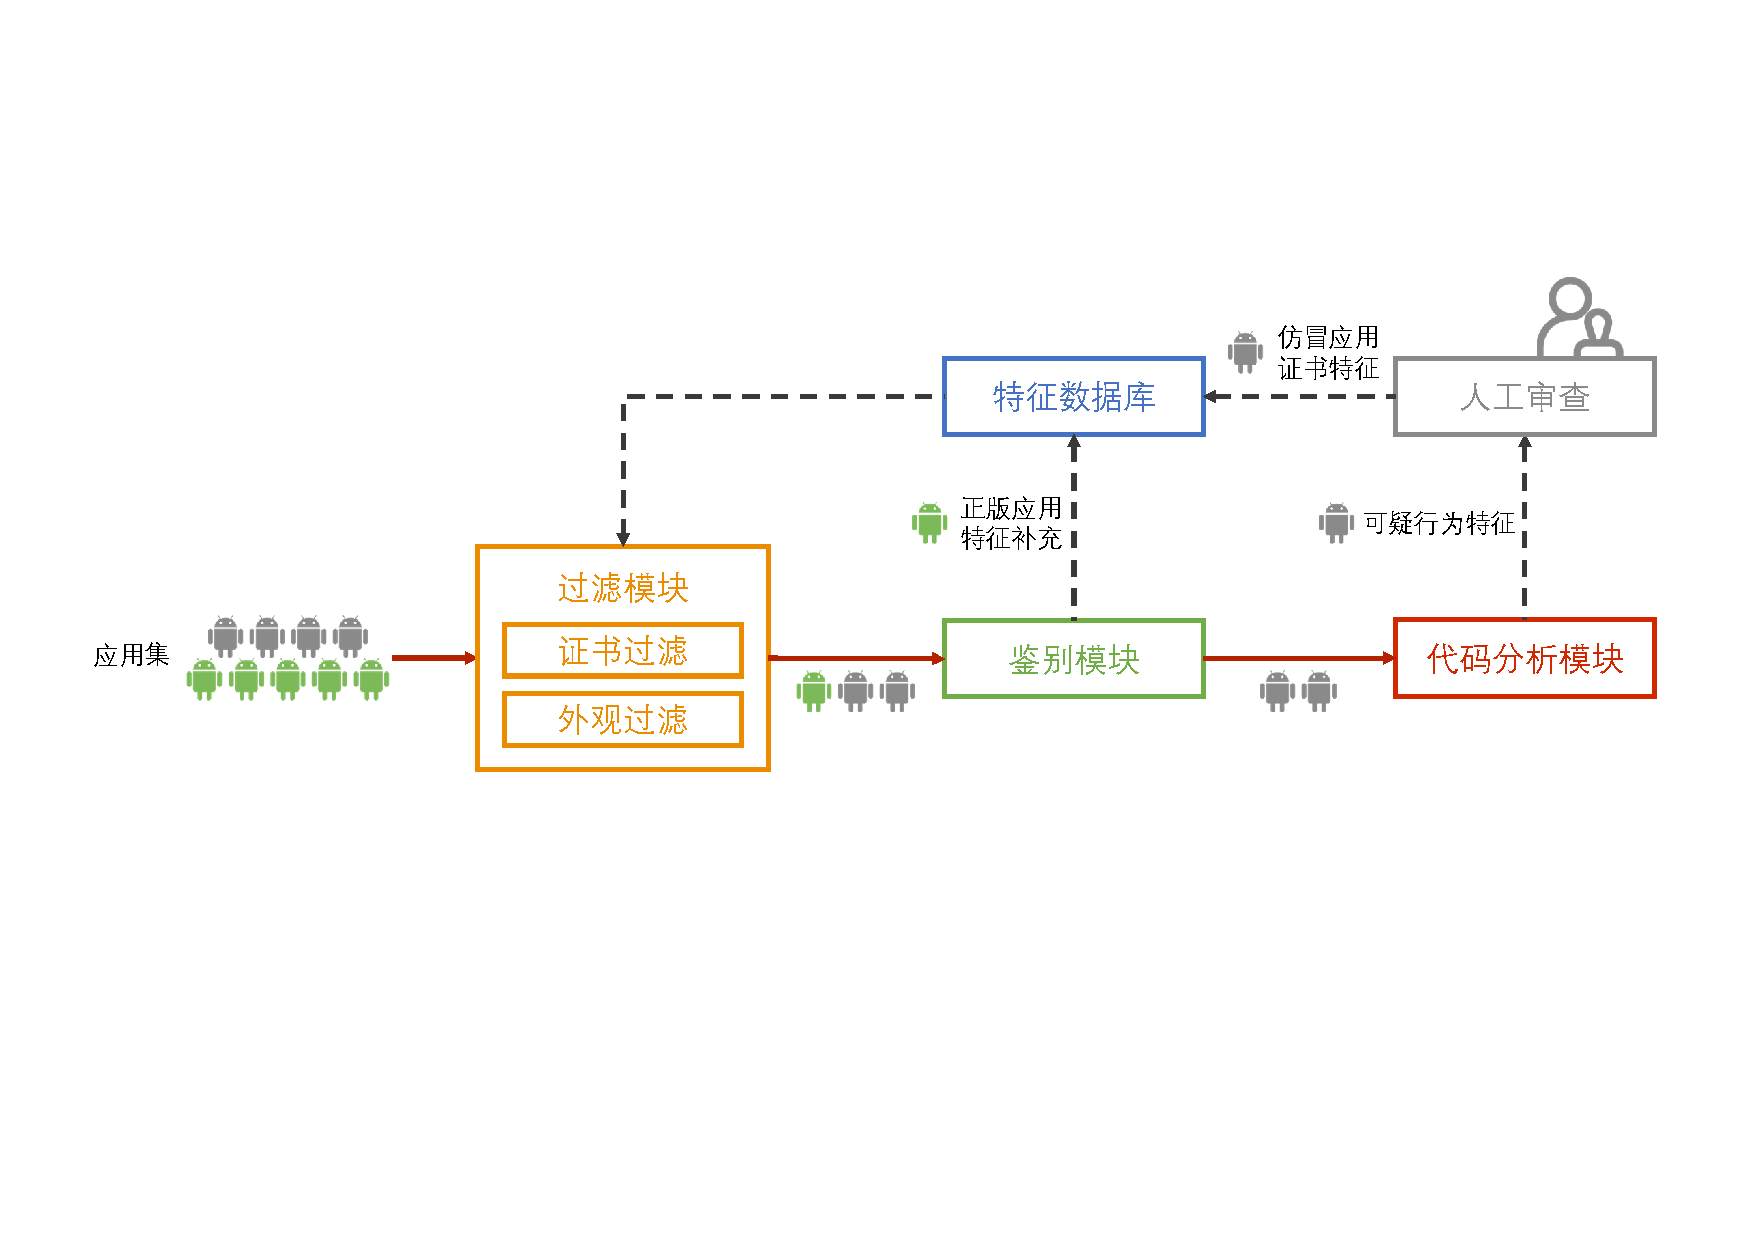
\includegraphics[width=\textwidth]{./Figures/edwin-fakerevealer-detector}
    \caption{\mytool 整体流程}
    \label{fig:Workflow_detector}
    \vspace{-3mm}
\end{figure}

\autoref{fig:Workflow_detector}展示了\mytool 的整体工作流程,框架主要分为\textbf{\componentA} 、\textbf{\componentB} 、\textbf{\componentC}、\textbf{\componentD} 和\textbf{\componentE} 五个部分。
\componentE 为存储应用特征的数据库,用户在使用前,需要先在\componentE 中输入部分正版应用特征信息和其他相关信息(如开发者黑名单)作为先验知识。
\mytool 以Android应用集为输入,先利用\componentA 对应用集进行初筛,过滤与正版应用不相关或相似度低的应用,降低后续检测与人工审核的压力。
之后,\componentB 提取应用样本的证书信息进行仿冒鉴别。
被判别为正版的应用样本的外观特征将被提取进\componentE 中以加强后续检测;被判别为仿冒的应用样本则会进入\componentC 被提取行为信息。
\componentC 提取应用中的静态分析数据(如应用代码中的方法信息、类信息等),构造方法调用图,分析应用的行为信息;此外,应用样本的基本信息也会被提取,方便后续展示。
之后,\componentC 分析涉及敏感API调用(如打电话、收发短信等)的应用行为,其中的可疑行为会被记录,汇总后分发到\componentD 环节复核。
Android应用面对的业务场景是十分复杂的,类似的方法调用行为在不同业务场景下会有截然不同的含义,因此现阶段仍需\componentD 确认应用的API调用是否可疑或具有恶意。
结合框架给出的应用信息和方法调用关系,应用市场审核人员可对仿冒应用进行快速判别,提高审核效率。
最后,在\componentD 环节确认为仿冒应用或恶意应用的样本的证书特征将被加入\componentE ,由同一开发者证书签署的其他应用在未来的检测中会在\componentA 阶段被直接拦截。

框架基于Python 3编写。

\subsection{\componentA }
\componentA 是一个预筛模块,有三个主要功能:
其一为通过应用证书信息比对,筛出黑名单开发者的应用,拒绝将其上架;
其二为通过将输入的应用与已知正版应用匹配,将与已知正版应用无关的输入滤除,减少后续检测压力;
其三为对输入的应用分类,以便在\componentB 中根据分类进行对应的正版检测。
\componentA 分为两部分,分别为\textbf{证书过滤}和\textbf{外观过滤}。

证书过滤指应用进入框架后,将先被提取证书信息,与\componentE 中已有的开发者黑名单比对,黑名单包含已知的恶意开发者证书信息。
若应用证书于黑名单内,该应用将被直接拒绝上架,流程结束。
证书信息比对部分的开发者黑名单由应用市场方自行维护,其中应包括已知仿冒开发者的证书信息与用于在Android Studio等开发环境调试的debug证书信息。
应用市场也应定期与其他各应用市场共享黑名单信息,防止\fullref{chp:discoveries_basic}中发现的仿冒应用开发者在多个市场中上传应用、利用debug证书上传应用等风险再次产生。

外观过滤则再分为应用名匹配与应用图标匹配两部分。
由\fullref{chp:discoveries_basic}总结可得,仿冒应用的命名与对应的正版应用十分接近,因此可利用应用名近似匹配寻找可能的仿冒应用;
应用图标匹配与应用名匹配交叉验证,减少对无关应用的误报。

在应用名匹配部分,判断输入应用是否与某一已知正版应用匹配的依据为正版应用命名模式。
一个正版应用的命名模式以不同特征点通过逻辑运算(与、或运算)连接而成,由用户提前给出,存入\componentE 中。

\begin{table}[htbp]
    \renewcommand{\arraystretch}{1}
    \footnotesize
    \centering
    \caption{\mytool 支持的应用名匹配特征点类型}
    \vspace{1mm}
    \begin{tabular}{l c}
        \toprule
        {\bf 特征点名}                 & {\bf 含义}                                 \\
        \midrule
        start\_with($str$)             & 应用名以字符串$str$开始                    \\
        end\_with($str$)               & 应用名以字符串$str$结束                    \\
        include($str$)                 & 应用名包含字符串$str$                      \\
        similarity($str$, $threshold$) & 应用名与字符串$str$的相似度大于$threshold$ \\
        max\_len($threshold$)          & 应用名长度不大于$threshold$                \\
        min\_len($threshold$)          & 应用名长度不小于$threshold$                \\
        \bottomrule
    \end{tabular}
    \label{table:name_pattern}
\end{table}

\autoref{table:name_pattern}展示了\mytool 目前支持的特征点类型。
比如,模式\textit{(start\_with(``开心'') and end\_with(``消消乐'') and max\_len(8)) or similarity(``开心消消乐'', 0.6)}将匹配到以``开心''为前缀、``消消乐''为后缀且应用名长度不大于8,或是应用名与``开心消消乐''相似度大于0.6的所有应用样本。
用户应根据对正版应用名的观察选择合适特征点,组成有效的正版应用的命名模式。

应用图标匹配部分,应用市场方需要先为已知正版应用配置一个图标和相似度阈值作为比较标准,\componentA 获取输入应用图标后,对两者进行相似度计算,若相似度大于等于阈值,则认为两者相似。
本框架采用了特征匹配算法计算图像相似度。

现有的常用图像相似度算法有严格判别算法、直方图比较、哈希算法和特征匹配法等。
严格判别算法即对两图片的像素点作严格一一比对的算法;
直方图比较则将两张图片的直方图数据归一化后比较两图相似度;
哈希算法会先将图片压缩,再为每张图片生成一个哈希串,通过哈希串之间对比实现图像相似度对比,可理解为将图像相似度转化为字符串相似度计算的算法;
特征匹配法则通过提取图像中的特征点,计算特征点的特征向量后,比对不同图像的特征向量进行相似度比对。
上述算法中,严格判别算法速度最快,但敏感度太高,鲁棒性并不好,只适用于严格判定图像全等的领域;
若仿冒开发者对原应用图标进行裁切、部分变色等变换处理,原图标的直方图会有较大变化,因此直方图比较算法也不适用于本场景。
哈希算法与特征匹配法是较适合本应用场景的对比方法,作者选择了特征匹配算法。

\begin{figure}[htbp]
    \centering
    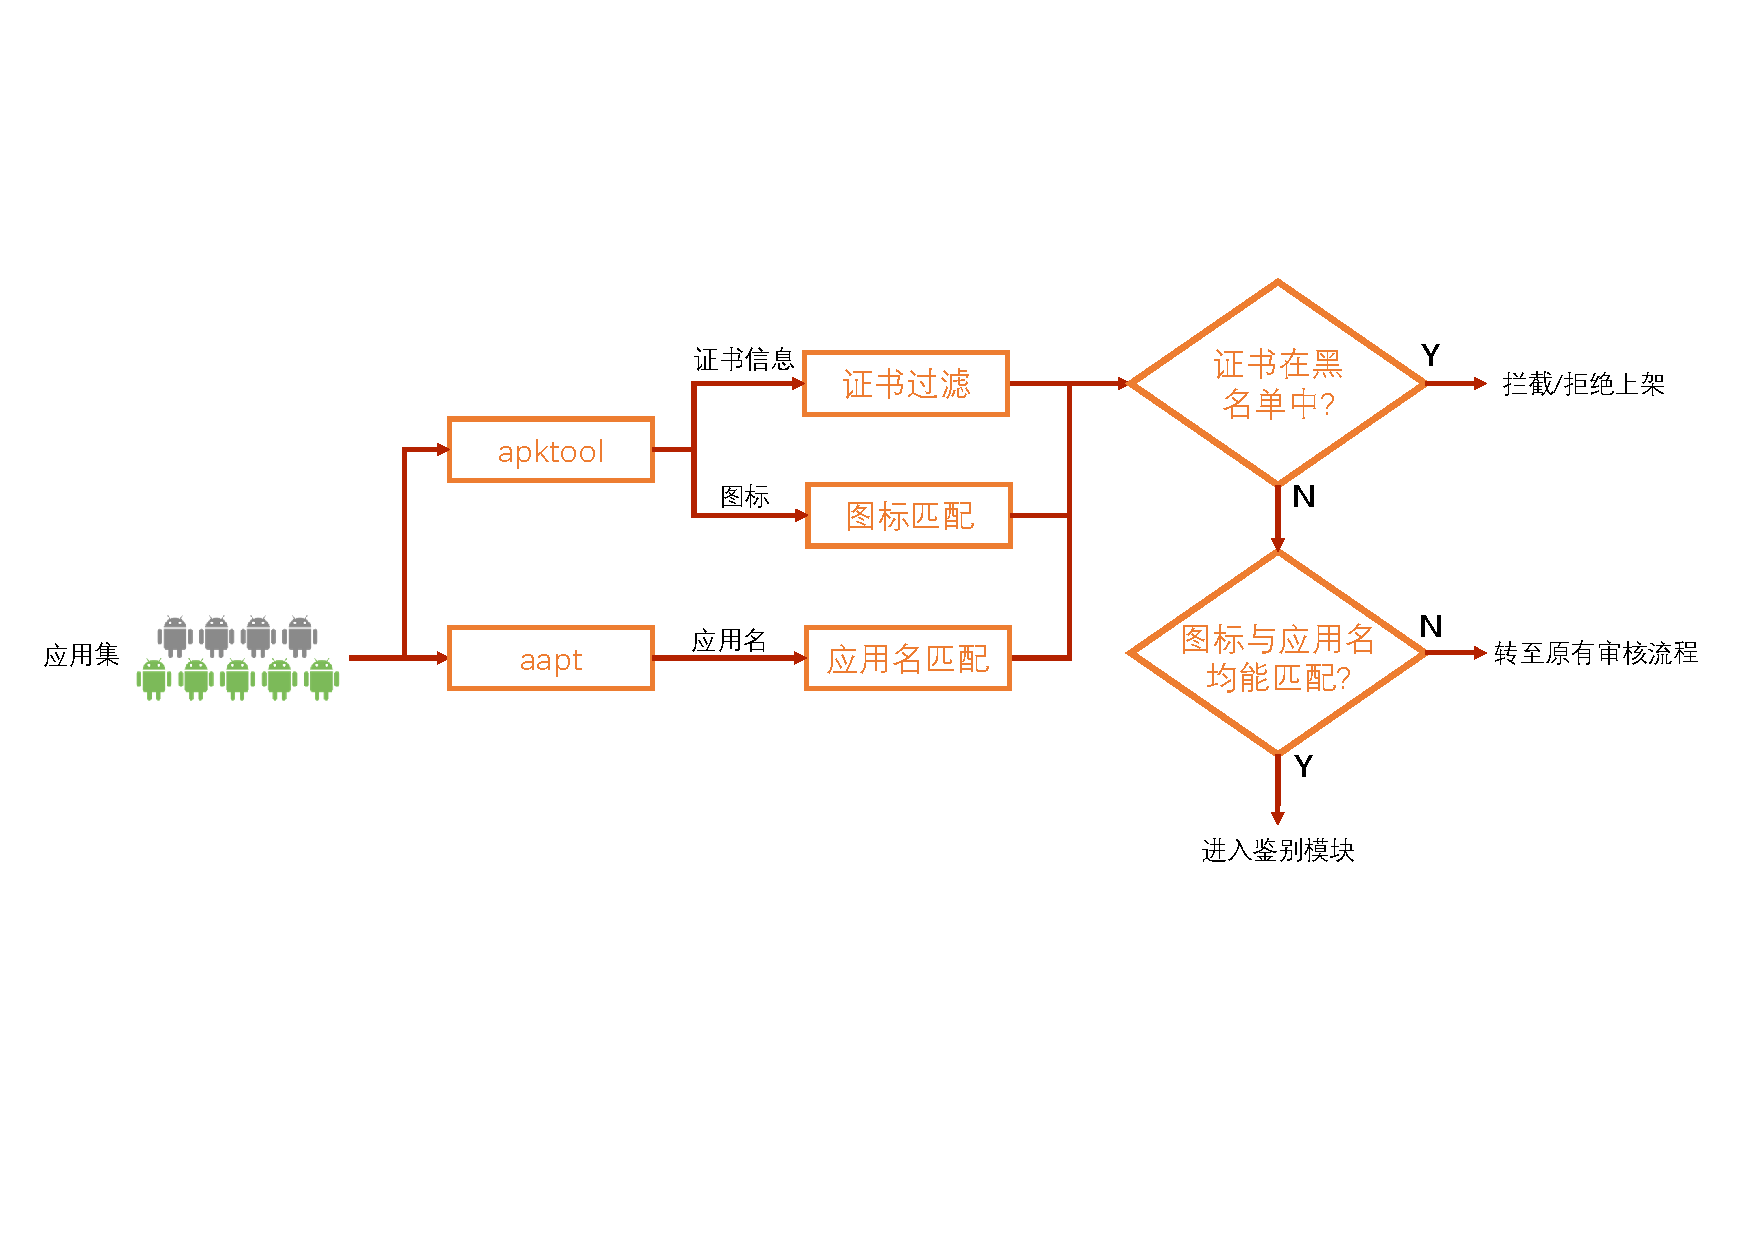
\includegraphics[width=\textwidth]{./Figures/edwin-component-A}
    \caption{\componentA 整体流程}
    \label{fig:workflow_componentA}
    \vspace{-3mm}
\end{figure}

\componentA 的具体实现流程可见\autoref{fig:workflow_componentA},证书信息在利用apktool对应用拆包后,使用JDK的keytool工具提取,APK中的图标文件具有固定路径,其提取也在apktool拆包后进行;
应用名提取由Android SDK中的aapt命令行工具对APK文件进行解析后,从解析结果中截取获得;
字符串匹配的相似度由两者之间的编辑距离与给出应用名的长度之比计算,特征匹配算法使用了图像的GIST(Generalized Search Tree)特征~\cite{torralba2003context}。

匹配之后,应用名和应用图标均被判定为与已知正版应用相似的样本会被打上对应标签(标记样本与哪个已知应用类似),进行后续的仿冒鉴别。
不被\componentA 判定为与已知正版应用相关、且应用证书不在开发者黑名单中的应用样本将进入应用市场方原有审核流程,而非由本框架判定是否仿冒应用或可否上架。

\subsection{\componentB }
\componentB 根据\componentA 的标签对应用进行进行仿冒鉴别,筛选应用集里的仿冒样本。
判别依据为样本内的证书指纹信息。
由\secref{sec:signature}可知,在大部分场景下,Android应用的签名信息指向应用的最后修改者,可直接通过签名信息甄别应用开发者。
然而,恶意开发者仍可利用在2017年被揭露的Janus漏洞,绕过V1机制签名,篡改APK文件。
因此,有必要对针对Janus漏洞进行额外检测,防止受攻击应用上架,妨害用户安全。
本小节将先简述Janus漏洞原理,再介绍本框架的检测手段。

\begin{figure}[htbp]
    \centering
    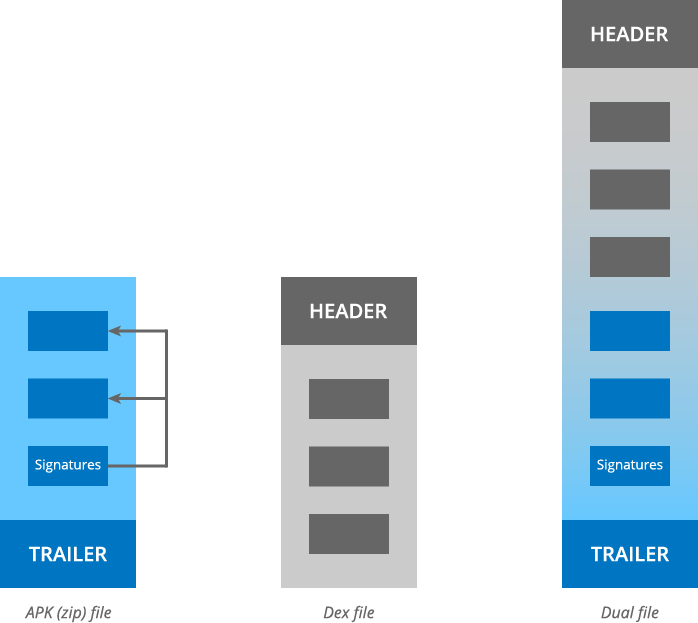
\includegraphics[width=0.7\textwidth]{./Figures/edwin-janus}
    \caption{Janus漏洞原理}
    \label{fig:how_janus_works}
    \vspace{-3mm}
\end{figure}

\autoref{fig:how_janus_works}\footnote{本图源于网络资料~\cite{CVE_2017_13156}}展示了Janus漏洞的工作原理。
在安装APK文件时,虚拟机先从APK的尾部(Trailer一端)读取校验签名信息(图中的Signature部分),校验成功后再从文件头部对APK文件进行解析和安装。
然而,Android系统的dex虚拟机同时支持对dex文件和apk文件的读取和执行。
若在APK文件头部拼接一个dex文件,虚拟机在完成新文件的尾部校验之后、跳转到文件头部对新文件进行解析安装时,将直接执行拼接于头部的dex文件,导致系统被攻击。

因此,对于使用V2、V3机制签名的应用,本框架直接利用应用的证书信息判别其是否仿冒应用;对于使用V1机制签名的应用,框架除验证证书信息外,还使用另一种手段确保应用未被攻击。
根据dex文件格式,每个dex文件的前8个字节为Magic number字段,内容为固定值``dex$\backslash$n035$\backslash$0'';而APK文件本质上为ZIP格式的压缩文件,也具有固定格式,文件头部的前4个字节内容为16进制的``504b0304''。
基于上述格式对文件头部前4个字节的内容读取判断,可鉴别应用是否损坏或被使用Janus漏洞攻击。

在本模块中被鉴别为正版应用的样本,其图标特征将被提取进\componentE 中以加强后续检测;若应用样本被认定为仿冒应用,则会进入\componentC 被提取代码信息。
利用Janus漏洞篡改应用的开发者将被直接加入\componentE 的开发者黑名单中。

\subsection{\componentC }

经过\componentA 和\componentB 对应用筛选鉴别后,\componentC 对应用进一步提取信息。
本模块提取的数据有两类,一类为应用的基本数据,另一类为应用的代码数据。
基本数据指应用的包名、构建应用使用的Android API版本、应用版本名称、应用版本号、应用大小、应用中声明使用的权限和证书指纹信息,以上信息可通过现有工具直接读取APK文件获取。
代码数据则指利用代码分析技术获取的数据。借助静态分析技术,\componentC 可从代码获取应用中的模块结构信息,包括应用中的类信息、各类中包含的方法信息、调用关系和应用写在\textit{AndroidManifest.xml}文件中的配置。
本模块在提取数据后,进一步分析调用关系,获取声明但未被使用过的敏感权限、敏感API调用链等信息,作为审核依据流转至\componentD 。

具体来说,\componentC 借助Androguard~\cite{Androguard},对应用中的dex文件进行反编译,获取反编译后的代码信息。
对dex文件反编译得到的Java代码中,按类的定义者区分,可将应用代码中包含的类分为三种类型,分别为系统类,用户自定义类和第三方类。
系统类指Android官方提供的开发框架中的类,如Android四大组件之一Activity的基类\textit{android.app.Activity};
第三方类指并非由Java语言本身提供、也并非开发者在项目中编写的类,通常包含于开发者引入的第三方库代码中,如游戏类应用常用Unity提供的第三方库作为游戏引擎;
用户自定义类指应用开发者在开发该应用时,于项目中自行编写定义的类(包括继承系统类的自定义类)。
Android Studio对应用项目进行编译打包时,会将部分系统类、项目中的所有第三方类和所有用户自定义类都编译进dex中。
对dex文件反编译出的所有代码进行解析会产生一定性能影响,也不利于应用间区分。
因此,\componentC 在处理时先使用Libradar~\cite{ma2016libradar}将系统类剔除和识别第三方类,一则减少后续分析的数据量,二则避免第三方类中的敏感API调用对后续分析产生影响。

\begin{algorithm}[!ht]
    \tablewuhao
    \caption{敏感API调用关系排查算法}
    \label{alg:dfs}
    \KwIn{ $permissions\_API$,列表,Android权限与API映射关系}
    \KwIn{ $decleared\_permissions$,列表,包含正版应用及其信息键值对}
    \KwOut{ $redundant\_permission$,集合,应用声明的冗余权限}
    \KwOut{ $calling\_sequence$,集合,分析后的敏感API的调用序列}
    \SetKwProg{Fn}{Function}{:}{}

    \Fn {iterSearcher($permissions\_API, decleared\_permissions$)} {

        $redundant\_permission \gets \emptyset$;

        \For {$permission \in decleared\_permissions$} {

            $flag \gets$ 0;

            \For {$API \in permissions\_API[permission]$} {

                $callers \gets $getCallers($API$);

                \If {not $caller$.is\_empty} {

                    $flag \gets$ 1;

                }

                \For {$caller \in callers$} {

                    $cache$ = PermissionCallAnalysis($caller$, $set(caller)$);

                    $calling\_sequence$.update($cache$);

                }
            }

            \If {$flag$ = 0}{

                $redundant\_permission$.add($permission$);
            }

        }
        \KwRet{$redundant\_permission$, $calling\_sequence$};

    }
\end{algorithm}

除了类信息,\componentC 还提取应用中的方法信息协助之后的人工审核。
提取的方法信息包括用户自定义的所有方法以及Android框架中较为敏感的方法调用信息。
用户自定义方法通过对Androguard中获得的用户自定义类进行方法分析获取:\componentC 遍历所有自定义类,获取其定义的每个方法,再将类名与方法名组合为二元组\textit{<class\_name, method\_name>},作为该方法在应用中的唯一标识保存;
敏感方法调用信息则以自底向上的方法进行排查。

在基本数据获取阶段,\componentC 通过aapt获得了构建应用的Android API版本和应用中声明使用的权限,而Androguard附带了各Android API版本中API与权限的映射关系。
结合以上信息可获取在某应用中可能会被调用到的敏感API,详情可见\autoref{alg:dfs}。
对于应用声明的每个权限,先通过映射关系查出其对应的敏感API列表;
对于每个敏感API,算法遍历应用中的各个用户自定义类和第三方类,排查应用中是否有对该敏感API的调用(第6行)。
如果有,则对调用该API的方法层层回溯,分析出敏感API的调用序列(第10行),具体流程见后文。
对于某个已声明的权限,如果其对应的全部敏感API均没有调用记录,则可对应两种情况:
一,该权限为由开发者声明的冗余权限,可能会被恶意应用利用,造成额外风险;
二,开发者通过Java反射机制调用了与权限对应的敏感API,导致该调用无法被静态分析扫描到。
无论是哪种情况,都可能对用户安全产生隐患,也可被视作风险点,因此\componentC 会记录该权限为冗余权限(第13行)。

\begin{algorithm}[!ht]
    \tablewuhao
    \caption{调用链回溯算法}
    \label{alg:trackback}
    \KwIn{ $cur\_method$,当前遍历的方法}
    \KwIn{ $itered\_methods$,集合,已遍历的方法}
    \KwOut{ $calling\_sequence$,集合,分析后的敏感API的调用序列}
    \SetKwProg{Fn}{Function}{:}{}

    \Fn {PermissionCallAnalysis($cur\_method, itered\_methods$)} {

    $calling\_sequence \gets \emptyset$;

    $callees \gets$ getCallees($cur\_method$);

    $callers \gets$ getCallers($cur\_method$);

    $cur\_seq \gets  []$;

    \For {$callee \in callees$} {
        \If{$callee$.is\_permission\_related\_API}{
            permission = $callee$.get\_related\_permission();

            $cur\_seq$.add($<callee, permission>$);
        }
    }

    \For {$caller \in callers$} {
        \If{$caller$.is\_self\_defined $\&\& caller \notin itered\_methods$} {
            $itered\_methods$.add($caller$);

            $res \gets$ PermissionCallAnalysis($caller, itered\_methods$);

            \For {$sequence \in res$} {

                $calling\_sequence$.add($sequence$ + $cur\_seq$);

            }
        }
    }
    \If {$calling\_sequence$.is\_empty $\&\&$ $cur\_seq$ != []}{

    $calling\_sequence$.add($cur\_seq$);

    }

    \KwRet{$calling\_sequence$};

    }

\end{algorithm}

在实现对敏感API调用链的回溯分析时,有两点挑战如下:
第一点是方法调用路径中可能会出现调用环;第二点是敏感API及其前序方法可能存在多个调用者。
前者指同一个方法多次出现在调用链中(如某方法多次递归调用自身后再调用敏感API),容易导致工具在进行调用链回溯时出现死循环;
后者让调用链成为了一棵以敏感API为根节点的调用树,树上的每个节点为一个方法,节点之间的有向边表示方法之间的调用关系。
方法调用并不是一个线性过程,各方法之间灵活的相互调用导致了以上两点挑战。

为应对以上两点挑战,\componentC 采用DFS算法和集合进行调用链回溯处理,具体可见\autoref{alg:trackback}。

对个某个方法,\componentC 先借助Androguard获取其所有被调用者(第3行)和调用者(第4行)。
如果被调用者中包含与权限相关的API,则将$<API, permission>$(即该API和其对应的权限)加入现有调用序列中(第6到9行)。
之后,对每个调用者,若其之前未被分析过,且其为用户自定义方法,则递归调用方法$PermissionCallAnalysis$回溯以该方法为起始点的权限相关API调用序列(第10至15行)。
对于方法是否被调用过的判断可以保证之前分析过的方法不再被重复分析,避免死循环的产生;
遍历调用者和递归调用$PermissionCallAnalysis$保证了所有调用者均可被回溯,若某方法没有被其他自定义方法调用、或是其调用者已经全被被分析过,则该方法为回溯终点。

分析结束后,\componentC 将应用信息汇总,流转至\componentD 。

\subsection{\componentD }

应用市场的审核人员在本模块对仿冒应用进行风险评估和确定。
尽管本框架的前三个模块自动化地进行了仿冒应用的判别和应用行为信息的获取,但应用的业务场景十分复杂,相同的API调用链在不同业务场景下可以有截然不同的含义(如``获取设备位置信息并上传至服务器''在导航软件中是必要的,而其他应用的相同行为可能会侵犯用户隐私),因此人工审查仍然不可避免。
此处的人工审查有两个作用,其一是对被鉴定为仿冒的应用进行确认,排除误报信息,并根据误报情况修正\componentA 中不同部分的匹配阈值;其二是对仿冒应用的行为进行风险评估,根据应用行为的风险大小决定对应用和对应开发者的处理。
如果一个样本仅在外观上模仿正版应用,但应用行为没有可疑之处,应用市场可驳回该次上架请求,要求开发者修正应用名与图标后重新申请上架;
然而,若样本的确包含高风险行为甚至包含恶意代码,应用市场除了拒绝上架该应用,还可以对应用开发者作封禁处理,将应用中的证书指纹信息加入\componentE 的黑名单中,在未来的检测中直接拦截相同证书签署的应用。

% 最后,\componentC 汇总各样本文件的检测结果并输出。
% 虽然框架在应用筛选、数据提取和规则判定上都实现了自动化,免去了审核方安装、运行应用或手动反编译APK等人工成本,但在应用量较大时,误判风险是无法避免的,需要由人工对结果进行复核确认。
% 每项规则都通过的样本被判别为正版应用,在经过人工确认后,其在\componentB 中被抽取的数据将会作为特征被存入\componentD 中。

% 同样需要人工的还有规则梳理部分。
% \secref{sec:func_and_behavior}显示,仿冒应用开发者在对不同类型的应用进行仿冒时,会有不同的行为特征,如\texttt{开心消消乐}的仿冒版本实际运行状况与正版相似,\texttt{王者荣耀}的仿冒则多为简单的拼图、壁纸等应用。
% 因此,人工审查的另一个作用在于观察被判定为仿冒应用的样本,为正版应用制订个性化规则,提高检测的准确率。

\section{系统实验}

上节介绍了框架的设计与实现,本节将介绍针对框架的实验设计和结果分析。

\subsection{数据收集}

为检验\mytool 的有效性,作者重新从Janus平台上收集了286个应用样本对\mytool 进行测试。
286个应用样本包含了采集自5个热门应用的255个样本和随机采集的31个噪声样本,详细分布可见~\autoref{table:exp_data_count}。

\begin{table}[htbp]
    \renewcommand{\arraystretch}{1}
    \footnotesize
    \centering
    \caption{\mytool 实验样本来源}
    \vspace{1mm}
    \begin{tabular}{l ccc}
        \toprule
        {\bf 来源应用} & {\bf 正版数量} & {\bf 仿冒数量} & {\bf 总计} \\
        \midrule
        抖音           & 32             & 18             & 50         \\
        开心消消乐     & 51             & 27             & 78         \\
        保卫萝卜       & 21             & 15             & 36         \\
        贪吃蛇大作战   & 14             & 29             & 43         \\
        WiFi万能钥匙   & 2              & 46             & 48         \\
        噪声应用       & N/A            & N/A            & 31         \\
        \bottomrule
    \end{tabular}
    \label{table:exp_data_count}
\end{table}

噪声样本用于检验\mytool 是否准确地在不产生应用误报(将无关应用识别为与已知应用相关的应用)的前提下,找到与已知应用有关的Android应用。
在\componentA 的图标匹配部分,算法效果可能受已知样本数影响。
框架为了消除该影响,实验在不同类别的应用中采用了不同的正版/仿冒数量比例作对比。

\subsection{实验与结果}

进行本组实验的设备搭载了Intel i5-8250 CPU与24GB内存。
由于已知研究中,与仿冒应用直接相关的资料较贫乏,对比实验以近似研究提出的工具(\secref{sec:study_repackaging}中的CodeMatch~\cite{CodeMatch})作为比较对象。
CodeMatch是利用第三方库信息检测重打包应用的工具,用户在使用前需先将已知第三方库信息加入数据库中。
工具先扫描APK文件获取代码,然后排除其中的已知第三方库,通过计算、比对剩余代码的哈希值进行重打包判断。
根据本文定义,重打包应用也属于一种仿冒应用,因而可采用CodeMatch进行对比实验。

\noindent{\bf 实验1:工具有效性验证}

本实验以上节的286个应用样本组成测试集。
\mytool 在使用前需先配置正版应用相关信息,作者从测试集的5种正版应用中各取2个正版样本,提取其应用图标中的特征作为先验知识存入数据库中,图标匹配的相似度阈值均设置为0.8,余下276个样本输入\mytool 进行测试。

\begin{table}[htbp]
    \renewcommand{\arraystretch}{1}
    \footnotesize
    \centering
    \caption{有效性实验判别结果统计}
    \vspace{1mm}
    \begin{tabular}{l ccccccc}
        \toprule
        \bf{来源应用}                  & \makecell[c]{\bf 正版样本识别数                                                     \\ \bf (TN)} & \makecell[c]{\bf 仿冒样本识别数 \\ \bf (TP/rgb)} & \makecell[c]{\bf 仿冒样本识别数 \\ \bf (TP/gray)} & {\bf FN} & \makecell[c]{\bf FP \\ \bf (rgb)} & \makecell[c]{\bf FP \\ \bf (gray)} \\
        \midrule
        抖音                           & 30                              & 15        & 17       & 0      & 3       & 1       \\
        \rowcolor{gray!15}开心消消乐   & 49                              & 24        & 24       & 0      & 3       & 3       \\
        保卫萝卜                       & 19                              & 10        & 11       & 0      & 5       & 4       \\
        \rowcolor{gray!15}贪吃蛇大作战 & 12                              & 29        & 29       & 0      & 0       & 0       \\
        WiFi万能钥匙                   & 0                               & 32        & 30       & 0      & 14      & 16      \\
        \rowcolor{gray!15}噪声应用     & 0                               & 0         & 0        & 0      & 0       & 0       \\
        {\bf 总计}                     & {\bf 110}                       & {\bf 110} & {\bf111} & {\bf0} & {\bf25} & {\bf24} \\
        \bottomrule
    \end{tabular}
    \label{table:exp_1_effectiveness}
\end{table}

\autoref{table:exp_1_effectiveness}展示了\mytool 对6种应用的辨识结果。
表中的``rgb''和``gray''分别对应图标匹配时采用的不同模式;``TP'',``TN'',``FP'',``FN''分别对应\textit{True Positive},\textit{True Negative},\textit{False Positive}和\textit{False Negative},用于描述实验结果。
因\mytool 用于鉴别仿冒应用,实验的``Positive''被设置成鉴别为仿冒的样本数目,``Negative''为鉴别为正版的样本数目(即``非仿冒样本''的数目)。

``rgb''模式表示采用包含rgb信息的原图像进行特征采集,``gray''模式表示在采集特征前先对图标进行灰度化处理。
在rgb模式下,每个像素点的色彩由``r'',``g'',``b''三个值表示,每个值的值域为$[0, 255]$,而在gray模式下,一个像素点的色彩只需用一个值域同为$[0, 255]$的值表示其灰度,因此在gray模式下进行的特征运算和比较速度更快。
结果表明,两种模式下的检测效果相当,gray模式甚至略优于rgb模式。
综合效果与运算速度,gray模式更适合本框架使用。
另外,\mytool 在两种模式下均能正确辨认所有正版样本,因此\autoref{table:exp_1_effectiveness}中的TN与FN不再分模式列出数据。

\begin{table}[htbp]
    \renewcommand{\arraystretch}{1}
    \footnotesize
    \centering
    \caption{实验准确率、召回率与F1值(单位:\%)}
    \vspace{1mm}
    \begin{tabular}{l ccccccc}
        \toprule
        \bf{来源应用}                  & \makecell[c]{准确率                                                                   \\(rgb)} & \makecell[c]{准确率\\(gray)} & \makecell[c]{召回率\\(rgb)} & \makecell[c]{召回率\\(gray)} & \makecell[c]{F1值\\(rgb)} & \makecell[c]{F1值\\(gray)} \\
        \midrule
        抖音                           & 83.33               & 94.44       & 100.0     & 100.0     & 90.91       & 97.14       \\
        \rowcolor{gray!15}开心消消乐   & 88.89               & 88.89       & 100.0     & 100.0     & 94.12       & 94.12       \\
        保卫萝卜                       & 66.67               & 73.33       & 100.0     & 100.0     & 80.0        & 84.62       \\
        \rowcolor{gray!15}贪吃蛇大作战 & 100.0               & 100.0       & 100.0     & 100.0     & 100.0       & 100.0       \\
        WiFi万能钥匙                   & 69.57               & 65.22       & 100.0     & 100.0     & 82.05       & 78.95       \\
        \rowcolor{gray!15}噪声应用     & N/A                 & N/A         & N/A       & N/A       & N/A         & N/A         \\
        {\bf 平均}                     & {\bf 81.48}         & {\bf 82.22} & {\bf 100} & {\bf 100} & {\bf 89.80} & {\bf 90.24} \\
        \bottomrule
    \end{tabular}
    \label{table:exp_1_accuracy_etc}
    \vspace{-3mm}
\end{table}

\begin{equation}
    Precision = \frac{TP}{TP+FP} \,,
    \label{equ:precision}
\end{equation}
\begin{equation}
    Recall = \frac{TP}{TP+FN} \,,
    \label{equ:recall}
\end{equation}
\begin{equation}
    F1 = 2\times \frac{Precision \times Recall}{Precision + Recall} \,.
    \label{equ:f1}
    \vspace{5mm}
\end{equation}

\autoref{table:exp_1_accuracy_etc}展示了\mytool 在本次实验的准确率(\autoref{equ:precision})、召回率(\autoref{equ:recall})和F1值(\autoref{equ:f1})数据。
\mytool 平均准确率分别为81.48\%(rgb模式)和82.22\%(gray模式),
没有对正版应用误判的记录,两种模式下的召回率均为100\%,
平均F1值则分别为89.80\%(rgb模式)和90.24\%(gray模式)。
总体上看,\mytool 整体可用性较好,在个别应用(\texttt{贪吃蛇大作战})下甚至可以识别出所有仿冒样本。
\mytool 不对正版错判的原因有两个,一个是于\secref{sec:signature}中介绍的Android签名机制,另一个是\componentB 将正版图标特征反馈回特征数据库的机制。
前者保证持有正版开发者证书的应用不会被误判为仿冒应用,后者保证\mytool 对新图标有一定容错性。

\begin{figure}[htbp]
    \centering
    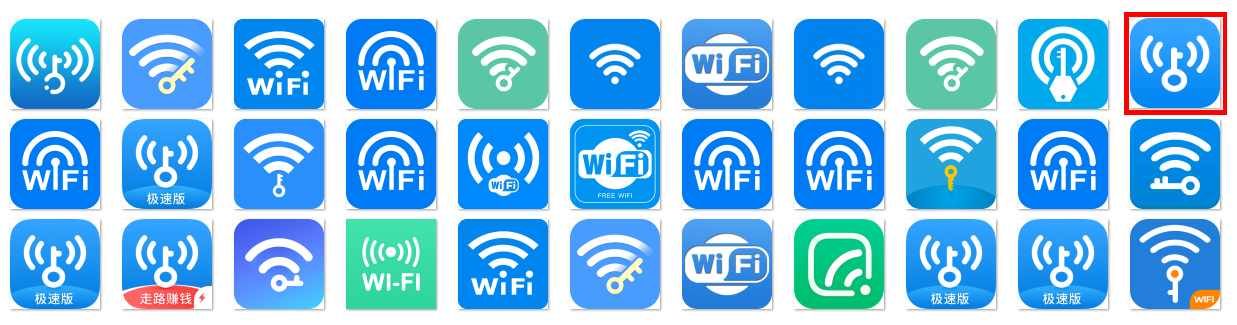
\includegraphics[width=\textwidth]{./Figures/edwin-exp-comparison}
    \caption{正版与仿冒版\texttt{WiFi万能钥匙}图标}
    \label{fig:exp_comparison_icon}
    \vspace{-3mm}
\end{figure}

然而,在\texttt{WiFi万能钥匙}应用下,\mytool 的鉴别能力较差,46个仿冒样本中有16个样本未被拦截。
人工确认结果显示,该部分样本均因为图标匹配未达阈值而被误判。
\autoref{fig:exp_comparison_icon}展示了\texttt{WiFi万能钥匙}对应的部分仿冒应用图标,正版图标于右上角由红色边框标出。
该结果表明图标匹配算法仍有改进空间。

为确保\mytool 仅对已知应用样本生效,测试集还包含了31个随机搜集的应用样本(噪声应用),该组样本的图标和应用名均与已知的5种应用不类似,用于测试\mytool 是否会对未收录的应用类别产生误报。
数据显示,31个噪声应用均未被判定为正版或仿冒,\mytool 具有一定抗干扰能力。

\begin{figure}[ht]
    \centering
    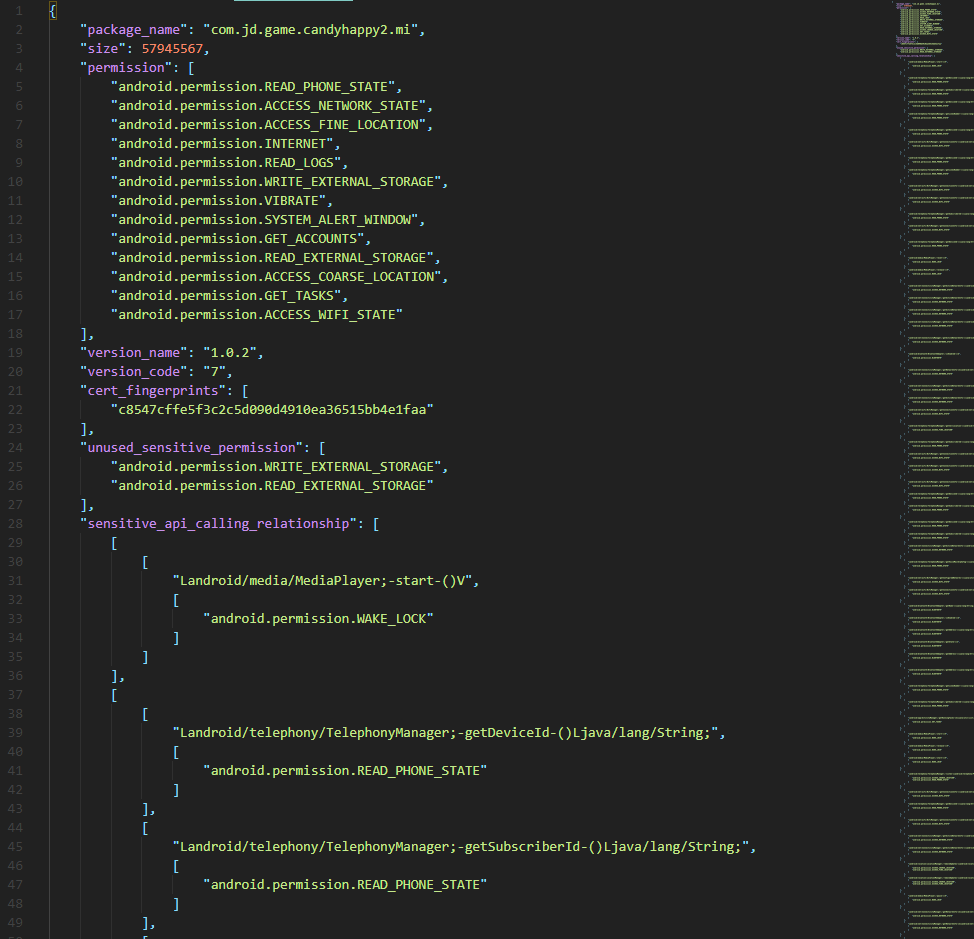
\includegraphics[width=\textwidth]{./Figures/edwin-component-C.jpg}
    \caption{\componentC 输出结果(局部)}
    \label{fig:componentC}
    \vspace{-3mm}
\end{figure}

\autoref{fig:componentC}给出了\componentC 针对其中一个仿冒样本的输出结果。
由于原输出数据量较大,此处不全部列出。
输出以Json字符串形式给出,有较清晰的结构性,在数据量较大的情况下也能易于查阅。


\noindent{\bf 实验2:对比实验}

本组实验用于比较CodeMatch与\mytool 在分析应用时的有效性,分为时效性对比与准确性对比。
实验采用\texttt{WiFi万能钥匙}、\texttt{保卫萝卜}与\texttt{开心消消乐}三组样本作为实验对象,测试两个工具是否能正确判别出输入中的仿冒样本。
CodeMatch的输入为两个APK文件组成的应用对,输出为两文件是否存在重打包关系,并不能直接判断某个应用样本是否仿冒。
因此,作者直接以应用的正版样本与对应仿冒样本组成的应用对作为CodeMatch的输入,两两比对,检查仿冒应用中是否存在正版应用的重打包样本。
\texttt{WiFi万能钥匙}组中包含2个正版样本与46个仿冒样本组成的92个应用对;
\texttt{保卫萝卜}组包含21个正版样本与15个仿冒样本组成的315个应用对;
\texttt{开心消消乐}组包含51个正版样本与27个仿冒样本组成的1377个应用对。
\mytool 方面则将三组应用的正版样本信息全部录入\componentD ,以对应的仿冒样本作为工具输入,图标匹配以gray模式进行。

\begin{table}[htbp]
    \renewcommand{\arraystretch}{1}
    \footnotesize
    \centering
    \caption{对比实验结果}
    \vspace{1mm}
    \begin{tabular}{l cccc}
        \toprule
        {\bf 工具名}               & {\bf 应用组别} & {\bf 运行次数} & {\bf 平均每次用时} & {\bf 发现的仿冒应用/重打包应用数} \\
        \midrule
        CodeMatch                  & WiFi万能钥匙   & 92             & 51.86分钟          & 0                                 \\
        \rowcolor{gray!15}\mytool  & WiFi万能钥匙   & 46             & 2.13分钟           & 30                                \\
        CodeMatch                  & 保卫萝卜       & 315            & 10.98分钟          & 0                                 \\
        \rowcolor{gray!15}\mytool  & 保卫萝卜       & 15             & 1.32分钟           & 11                                \\
        CodeMatch                  & 开心消消乐     & 1377           & 23.61分钟          & 27                                \\
        \rowcolor{gray!15} \mytool & 开心消消乐     & 27             & 1.40分钟           & 24                                \\

        \bottomrule
    \end{tabular}
    \label{table:exp_2_comparison}
\end{table}

实验结果可见\autoref{table:exp_2_comparison}。
在\texttt{开心消消乐}组,CodeMatch在863个应用对中发现了重打包关系,经筛选去重后整理出27个仿冒样本(表示本组应用所有仿冒样本均为重打包应用),展示了其有效性。
然而,CodeMatch并未能从\texttt{WiFi万能钥匙}与\texttt{保卫萝卜}两组应用的仿冒样本中检查出异常,即两组的仿冒样本中均未包含对正版样本的重打包应用。
\mytool 的表现较为稳定,判别结果与实验1中结果一致。
上述实验结果说明,重打包应用检测在仿冒应用为重打包应用的特定场景下有较好的命中率,但该方法不适用于大规模的仿冒应用鉴别。
受检测原理限制,检测重打包应用要对所有正版样本与所有未知样本两两比较,在样本量较大时会产生极大计算量(可见\autoref{table:exp_2_comparison}``运行次数''一列)。
最重要的是,重打包应用只是仿冒应用的一种,使用重打包检测方法检查仿冒应用会遗漏非重打包形式的仿冒应用,缺乏灵活性。
仿冒应用凭借外观迷惑用户,检测方应该以应用名和图标鉴别仿冒应用,因而\mytool 的整体有效性高于CodeMatch。

用时方面,由于重打包应用需要在获取应用代码之后将代码和数据库中的所有已知第三方库逐一比对,故CodeMatch的每次运行时间开销明显高于\mytool ;
相比之下,\mytool 直接根据应用名模式与图标特征对应用进行筛选,主要时间开销用于对仿冒样本的分析中,需处理的数据量远小于重打包检测中逐行代码比对产生的数据量,因此在速度上占优。
此外,CodeMatch只能告知用户两个应用是否具有重打包关系,并未给出更多相关信息,而\mytool 利用\componentC 分析APK文件后,以Json格式输出结构清晰的分析结果,方便审核人员验证判别有效性。

综上,作者认为\mytool 在仿冒应用检测上优于CodeMatch。
重打包检测并非检测仿冒应用的有效思路,以应用外观为依据检测仿冒应用是更有效且快捷的方法。

% \section{已知相关工具}

% 根据研究前期文献查阅结果,在移动应用领域,针对仿冒应用进行的研究较为缺乏,因此未有其他仿冒应用检测可与本框架进行横向比对。
% 在近似的研究领域(重打包应用检测)中,CodeMatch~\cite{CodeMatch}和Wukong~\cite{Wukong}均对应用代码中的第三方库代码信息进行了分离处理。
% CodeMatch在剔除第三方库代码后,通过计算比对余下代码的哈希值判断应用相似度,Wukong则使用了基于计数的代码克隆检测手段,而非基于哈希的技术。
% 类似地,本框架的\componentB 中也有对自定义代码和第三方代码的分离收集。
% 然而,\componentB 仅负责数据提取,分离收集第三方代码是为了能向用户提供更充分的数据,以便用户编写规则进行判定,因此无法直接与上述工具比对。
% 在\componentB 可提供静态分析数据的前提下,作者在本框架上根据CodeMatch的思路,将其复现于规则3上。

\section{本章小结}

本章介绍了仿冒应用检测框架\mytool 的设计与实现,并对其进行了系统实验。
\mytool 是设计用于Android应用市场的仿冒应用检测框架,有五个主要部分,用于自动化拦截对已知正版应用进行仿冒的仿冒应用和已知恶意开发者的恶意应用,可减缓应用市场在应用审核方面的人力成本,提高应用市场的安全程度。
Android应用市场常有大量应用上传等待上架,为有效处理大批量Android应用程序,\mytool 采用\componentA 对应用进行快速筛选,剔除与已知正版应用不相似的应用样本,并为匹配的应用贴上对应标签。
\componentB 根据应用标签,鉴别应用真伪。
其后,\componentC 对\componentB 鉴别为仿冒的应用进行拆包反编译处理,采集包括应用包名、版本号、声明权限在内的基本数据与应用中的类信息、方法信息等代码数据传入\componentD ,并在人工确认后,将仿冒应用的证书指纹存入\componentE ;
由\componentB 判别为正版应用的样本将会被提取图标特征并加入\componentE 中,加强之后的检测。

系统实验显示,\mytool 具有较好的可用性,可利用较少的已知数据快速定位输入应用集中的仿冒应用,每个仿冒应用的判别与分析均可在数分钟内完成。
然而,部分仿冒应用因图标相似度未达到阈值未被\mytool 拦截,该结果表明\mytool 的图标匹配部分仍有改进空间。

\clearPaperPage

\chapter{总结与展望}
\label{chp:future}

\section{总结}
% In this paper we first introduce the concept of fake apps, and study specifically towards these apps.
在本文中,``仿冒应用''这个概念被率先引入。
然后,本文对这一方面进行了专门的研究,还搜集了大量的相关样本以辅助调查。
% To the best of our knowledge, we are the first to conduct a comprehensive empirical study on a large-scale fake apps.
本文的前期调研结果显示,本课题是第一个针对仿冒应用进行大规模全面实证研究的课题。

% To better understand the ecosystem nature of this type of apps, we obtained more than 150,000 data entries from real-world markets, observed and measured the fake samples among this dataset from several dimensions including certificate information, app size, app name and package name, time factor and so on.
为了更好地了解这个类型的应用的生态环境,本文基于Python 3设计实现了仿冒应用收集框架\mytool,利用基于BFS的算法收集了来自现实世界中各个应用市场的近14万个应用样本,并且从多个不同维度,对这个数据库里面的仿冒样本进行了观测和考察。
这些维度包括了APK包中的安全证书信息、应用大小、应用名、包名和时间因素等等。

% Through our measurements we gain valuable experience on fake apps from several perspectives, findings like fake samples' naming tendency and fake developers' evasive strategies are inferred.
然后,本工作将收集到的数据分为了\emph{仿冒应用的基本特征}、\emph{影响仿冒应用数量的因素}和\emph{仿冒应用的发展轨迹}三个不同视角进行了测量,获得如仿冒应用的命名倾向和仿冒应用开发者对市场监管防御机制的规避策略等信息。
% To support our findings, we further present a few study cases which provide us a more detailed look into fake apps to back our discoveries on fake app ecosystem.
为了佐证本文的发现,本研究在每个视角解读之后给出了从数据集中挑选的几个研究案例,呈现了如仿冒应用开发者对不同热门应用的仿冒方式的内容。
这几个案例进一步深化了本文对仿冒应用生态系统的发现。

之后,本文还收集了部分仿冒样本在商场上对应的评论和评级,排查仿冒应用是否利用了排名欺诈。
由于现有的排名欺诈检测手段尚有不足,本工作创新性地分别利用两种创新的研究方法---基于用户行为的用户可信度验证和基于NLP的评论内容相似度验证,对数据中的排名欺诈行为进行了排查。
结果显示,刷好评的排名欺诈行为的确存在于应用市场中,在本工作搜集到的仿冒应用评论中就有刷好评的痕迹。


\section{展望}

在大规模分析的部分中,本文中用到了三个不同的角度分别探索仿冒应用的特征,但回顾探索过程,一些方法和步骤依然不够深入。
如果能从以下三个角度再向仿冒应用入手研究,或许能有更多有所裨益的发现:

\begin{itemize}
    \item 应用图标:
    本文在进行案例研究中发现,不少仿冒应用的图标和原版官方应用的图标其实十分相像。
    因此,图标也可以是一个用于发掘/鉴别仿冒应用的突破口,研究者也许可以从应用图标中挖掘到更多可用的信息与行为模式。
    碍于时间因素所限,本文研究中并未加入图像对比处理部分提取各APK包中的图标与官方应用的图标进行比对,但如果能研究出快速比对多个应用间图标、图像相似度的算法,定当对应用市场的安全监管筛选机制有所好处。

    \item 应用内代码/文本/链接/ip分析:
    代码分析可以有效地剖析应用的行为,而相似的文本资源、链接等信息也可以提供各个App之间可能存在的关联关系。
    遗憾的是,从当前技术水平出发,仔细地对一个App进行完整而全面的静态分析所需时长太长,而动态分析需要测试样例驱动,自动化的动态测试工具往往未能深入拓展一个应用的大部分核心功能。
    因此,开发出快速的分析算法对App进行更深入的探索,就能挖掘出有关仿冒应用生态的更多信息。

    \item 仿冒应用总量的变化原因:
    \fullref{chp:discoveries}中提及到了Janus收集到的仿冒应用数量并非一直保持上升趋势。
    近年来,能搜集到的仿冒应用数量有突然下跌、甚至渐渐式微的迹象。
    究竟是什么因素导致了这个原因?是移动黑灰产内部的变化,还是安全厂商日益紧密的封锁?
    这将会是一个十分有趣的课题。
\end{itemize}

而在评论分析的部分中,也有可以继续发掘的部分。
在现阶段,学界关于排名欺诈的研究一直在针对积极评价方面,但是对应用差评进行排名欺诈的相关研究却有待补充。
刷好评可以提高应用评价提升应用排名,如果反其道而行之,用差评对目标应用进行攻击,其实也可以降低目标应用的评价,对其排名进行打击。
另外,在实际上,用户给的差评中含有相当多的有用信息。
用户对应用的不满、功能上的建议、bug的反馈,都可以反映在差评上。
关于用户差评,还有很多的研究空间。

最后,\mytool 框架本身,无论是代码层面还是设计层面,也有值得改善的地方。
比如是否能结合自动化爬虫框架提高爬虫模块的鲁棒性(对抗应用商店的反爬虫技术、下载稳定性),工具本身的代码优化,还有工具整体的易用性、稳定性等。

总之,从整体上看,本文的工作还有很多可以深化的部分。
然而,诚希望本文研究的结果能够为移动安全产业的从业人员(不论是工业界或学术界)提供足够的信息,以改善移动安全界的现状;或是抛砖引玉,在让读者对移动应用黑色产业有更多认识的同时,激发读者对仿冒应用等方面的研究兴趣,并从上述几点出发,为后人带来更多深入而完善的相关研究。

\clearPaperPage

% 参考文献
% 前置\cleardoublepage\phantomsection 以确保目录超链接到正确页码
\phantomsection\addcontentsline{toc}{chapter}{\small{参考文献}}
\bibliographystyle{GBT7714-2005}
\bibliography{bib/REFERENCE}
\clearPaperPage

% 攻读学位期间发表的学术论文
\fancypagestyle{plain}{%
    \fancyhead[LE,RO]{\small{\articleCategory}}
    \fancyhead[RE,LO]{\small{攻读学位期间发表的学术论文}}
}

\fancypagestyle{plain}{%
	\fancyhead[LE,RO]{华东师范大学硕士专业学位论文}
	\fancyhead[RE,LO]{ 攻读学位期间发表的学术论文}
}



\chapter*{攻读学位期间发表的学术论文}


\addcontentsline{toc}{chapter}{攻读学位期间发表的学术论文}


%\vskip 5mm

%{\heiti $\blacksquare$ 已公开发表论文}\vskip 5mm

\begin{enumerate}
	
	\item Chongbin Tang, Sen Chen, Lingling Fan, Lihua Xu, Yang Liu, Zhushou Tang, and Liang Dou, ``A large-scale empirical study on industrial fake apps,'' in \textit{Proceedings of the 41st International Conference on Software Engineering: Software Engineering in Practice,} IEEE Press, 2019: 183-192. (发表于CCF A类推荐学术会议, 软件工程方向顶级会议ICSE2019)
	
\end{enumerate}



\clearPaperPage

\fancypagestyle{plain}{%
    \fancyhead[LE,RO]{\small{\articleCategory}}
    \fancyhead[RE,LO]{\small{致\quad 谢}}
}
% 致谢。匿名与非匿名用不同版本
\ifx\anonymous \undefined
    \chapter*{ 致\qquad 谢}

\addcontentsline{toc}{chapter}{致  谢}




\vspace{0.2cm} \hspace{11.5cm}

\hspace{10.6cm}  二〇二〇年五月

\else
    \chapter*{ 致\qquad 谢}

\addcontentsline{toc}{chapter}{致  谢}

在师大的七年时光转瞬而逝,不知不觉,研究生历程已快要告一段落,我也将迎来下一个人生阶段。

借此机会,想对在师大遇上的各位老师和同学表示最真诚的感谢,尤其是我的导师,在我研究生的各个阶段都给予我鼓励和指导。同样想感谢的还有家里人和身边的朋友,是他们的支持帮助我走过了一路上的各种波折。


\vspace{0.2cm} \hspace{11.5cm}

\hspace{10.6cm}  二〇二〇年三月

\fi
\clearPaperPage


\end{document}
